%\documentclass[10pt]{book}%
\documentclass[letterpaper,openright,11pt]{article}

%PACKAGE%
\usepackage{blindtext}
\usepackage{geometry}
\usepackage{fancyhdr}
\usepackage{helvet}
\usepackage[spanish,es-tabla]{babel}
\usepackage[breaklinks=true]{hyperref}
\usepackage{multirow}
\usepackage{apacite}
\usepackage{booktabs}
\usepackage[utf8]{inputenc} 
\usepackage{anysize}
\usepackage{varioref}
\usepackage{enumerate}
\usepackage{graphicx} % Required for including images
\usepackage{amsmath}
\usepackage{wrapfig}
\usepackage{appendix}
\usepackage{pdfpages}

%CONFIGURACIONES%
\renewcommand{\familydefault}{\sfdefault} 
\setcounter{secnumdepth}{3} %para que ponga 1.1.1.1 en subsubsecciones
\setcounter{tocdepth}{3} % para que ponga subsubsecciones en el indice
\renewcommand{\baselinestretch}{1,5} %Interlineado
% Clear the header and footer
\pagestyle{fancy}
\fancyhead{}
\fancyfoot{}
\fancyfoot[R]{\thepage}

% we use \prefix@<level> only if it is defined
\makeatletter
% we use \prefix@<level> only if it is defined
\renewcommand{\@seccntformat}[1]{%
  \ifcsname prefix@#1\endcsname
    \csname prefix@#1\endcsname
  \else
    \csname the#1\endcsname\quad
  \fi}
% define \prefix@section
\newcommand\prefix@section{CAPITULO \thesection. }
\makeatother
\graphicspath{{Figures/}} % Set the default folder for images

%MARGENES
\marginsize{4cm}{2.5cm}{2.5cm}{2.5cm}

%Estilo del número de pagina
\pagestyle{fancy}
\fancyhf{}
\fancyheadoffset{0cm}
\renewcommand{\headrulewidth}{0pt} 
\renewcommand{\footrulewidth}{0pt}
\fancyfoot[R]{\thepage}
\fancypagestyle{plain}{%
   \fancyhf{}%
   \fancyfoot[R]{\thepage}%
}

%ANEXO
\renewcommand{\appendixname}{ANEXO}
\renewcommand{\appendixtocname}{ANEXO}
\renewcommand{\appendixpagename}{ANEXO}
%\renewcommand{\sectiontitle}\prefix@section{CAPITULO \thesection. }

%DOCUMENTO%
\begin{document}
\renewcommand{\figurename}{Fig.} %Cambia la palabra "Figura" por "Fig."
\renewcommand{\tablename}{Tabla} %Cambia la palabra "Cuadro" por "Tabla"
\renewcommand\thefigure{\arabic{section}.\arabic{figure}} % Genera numeración X.Y
\renewcommand\thetable{\arabic{section}.\arabic{table}} % Genera numeración X.Y
\numberwithin{figure}{section} %Hace que la primera figura de cada sección X sea X.1
\numberwithin{table}{section} %Hace que la primera tabla de cada sección X sea X.1
\bibliographystyle{apacite}

\renewcommand{\listtablename}{ÍNDICE DE TABLA}
\renewcommand{\listfigurename}{ÍNDICE DE ILUSTRACION}
\renewcommand{\contentsname}{TABLA DE CONTENIDO}
\renewcommand{\refname}{REFERENCIA BIBLIOGRÁFICA}


\begin{titlepage}

\begin{center}
	\vspace*{-1in}
	\begin{center}
	
		UNIVERSIDAD DE SANTIAGO DE CHILE\\
		\vspace*{0.15in}
		FACULTAD DE INGENIERÍA \\
		\vspace*{0.6in}

		\begin{figure}[htb]
			\begin{flushright}
				
\includegraphics[width=4cm]{./logo}
			\end{flushright}
		\end{figure}

	\end{center}	
	

	\vspace*{0.2in}
	
	\begin{Large}
		\textbf{Título: Actas dialógicas, circulación del conocimiento, recuperación del contexto como medio para tener reuniones efectivas} \\
	\end{Large}
		\vspace*{0.3in}

	\begin{large}
		Oliver Sergio Hidalgo Leal
	\end{large}
	
	\vspace*{0.3in}
	\vspace*{0.1in}
	
	\begin{large}
		Profesor Guía: Edmundo Pablo Leiva-Lobos \\
		Tesis de grado presentado en conformidad a los requisitos para obtener el grado de Magíster en Ingeniería Informática \\
	\end{large}

	\begin{center}
		Santiago-Chile \\
		2018
	\end{center}
	
\end{center}
\end{titlepage}
\newpage
\thispagestyle{empty} % para que no se numere esta pagina
\begin{flushleft}
\vspace*{\fill}
\textbf{©Oliver Hidalgo Leal,  2018}\newline
Todos los derechos reservados. Queda prohibida la reproducción total o parcial sin la autorización previa y por escrito.
\vspace*{1cm}
\end{flushleft}
\pagenumbering{Roman} 
\begin{center}

\textbf{\large{RESUMEN}}

\end{center}

El objetivo principal de la tesis, se justifica por el problema de las altas horas improductivas que se pasan en reuniones con casi ningún marco conceptual para enfrentar este gran dilema que es ubicuo en el mundo. Se propone una minuta electrónica, llamada D-Minute, para sostener reuniones eficaces donde cada participante de la reunión genere la colaboración y coordinación de actividades mediante los elementos de diálogo: duda, desacuerdo, norma, acuerdo y compromiso individual de forma tal que facilite el retomar el estado de reuniones pasadas. 

La tesis adopta el enfoque diálogo/acción para entender las reuniones en las cuales se articula el lenguaje con la acción en el proyecto mismo. Además, este enfoque caracteriza tantos los momentos de convergencia como los momentos de divergencia y los relaciona con tareas derivadas del acto de reunirse.  Se postula que el registro de estos momentos y sus elementos asociados, facilita el retomar el estado de reuniones pasadas de manera eficaz y expedita.

La metodología para desarrollar la tesis tiene tres fuentes I+D+i. En la práctica, la investigación entrega un diseño experimental para validar la eficacia de D-Minute con un experimento científico con dos equipos de proyectos - uno de control y otro experimental - para alegar mejoras basados en los tiempos de respuesta y circulación del conocimiento. La parte de innovación entrega un \textit{benchmark} con \textit{meetingware} existentes para justificar que D-Minute es un producto mínimo viable, con valor para un potencial segmento de clientes. De hecho, usando \textit{Lean} Canvas se pudo generar un modelo liviano de negocios usando la metodología \textit{Running Lean} que pone de relieve este hecho. Finalmente, la parte D es el \textit{meetingware} mismo D-Minute. En la creación del producto se utilizó: \textit{Scrum} como metodología de desarrollo de \textit{software}, Netflix OSS como arquitectura de \textit{Back-End}, Angular 5  como \textit{framework} para \textit{Front-End} y \textit{Docker} para el despliegue de micro servicios.\\

\begin{flushleft}
\textbf{Palabras Clave:} Trabajo Colaborativo, Diálogo, \textit{Meetingware}
\end{flushleft}
\begin{center}
\textbf{ABSTRACT}
\end{center}


Se concluye por el lado de la innovación un Lienzo Canvas para el modelo de negocio del mínimo producto viable, por el lado de la investigación el diseño del experimento que debe ser llevado a cabo para validar las hipótesis que dieron origen al \textit{software} D-Minute y por último una base para trabajos futuros.\newline 
\newline\textbf{Palabras Clave:} Trabajo Colaborativo, Diálogo, \textit{Meetingware}
\begin{center}
\textbf{AGRADECIMIENTO}
\end{center}

Ha sido un largo camino, uno lleno de muchos desafios, muchos objetivos que cumplir y muchas ilusiones. Sin embargo, en el proceso siempre me he sentido apoyado, tanto de mi familia como de mis amigos. El mirar hacia atras para ver como se cncluye este hito me hace recordar con emoción la historia, los origenes y me abre un camino de luz hacia donde deseo enfocar mi vida. No es simplemente el termino de una tesis, es cerrar un capitulo de tu vida al cual le dedicaste tiempo, te entrego alegrias y tristesas, te ilusiono y te dio otra perpestiva de la vida.

En mi vida he recorrido diferentes caminos, muchos de los cuales no han sido los mas agradables. Pero uno de ellos me ha llevado a escribir estas palabras a sentirme pleno en la vida a querer ser mejor cada día. En ese camino estan ustedes, mi mujer y mis hijas. Este trabajo es por ustedes y por mi, cuando en un futuro vean estas lienas recuerden que solo con amor es posible construir y solo con amor podemos hacer mejor nuestras vidas, ustedes llegaron a mi vida a entregar ese amor y con amor ...

\tableofcontents % indice de contenidos

\cleardoublepage
\listoftables % indice de tablas 

\cleardoublepage
\listoffigures % indice de figuras


\section{INTRODUCCIÓN}
\pagenumbering{arabic}

Este capítulo presenta una introducción y panorama general de la tesis de magíster, la cual propone un nuevo tipo de actas de reuniones basada en una teoría del diálogo llamada diálogo/acción. Primero, se da una descripción del problema propuesto y después la respuesta o solución a esa problemática. A continuación, se muestran los alcances del modelo de desarrollo para lograr una solución de software. Finalmente, se describe brevemente el contenido de los siguientes capítulos.


\subsection{ANTECEDENTES Y MOTIVACIÓN}
El área del CSCW\footnote{Para ver la definición de \textit{Computer Supported Cooperative Work} en este enlace \url{https://en.wikipedia.org/wiki/Computer-supported_cooperative_work}} es un campo multidisciplinario de investigación sobre el fenómeno de la colaboración y su relación con la tecnología informática. En ese campo se han desarrollado tecnologías como: sistema de videoconferencia, pizarras compartidas, sistema de intercambio, flujos de trabajo (en Inglés, \textit{workflow}); todas con enfoque de apoyo colaborativo al trabajo en grupo \fullcite{RN32}. A su vez, se ha han desarrollado marcos teóricos sobre actividades de trabajo en equipo como la presentada en \fullcite{RN24} que propone un enfoque llamado diálogo/acción\footnote{El diálogo/acción es una extensión del enfoque de lenguaje/acción propuesto originalmente por Terry Winograd y Fernando Flores (1986) y presentado en su libro “Understanding Computers and Cognition”. La diferencia principal entre ambos enfoques es que en lenguaje/acción centra exclusivamente en la parte estable de las conversaciones, es decir en los compromisos y los acuerdos. En cambio, en el enfoque diálogo/acción incorpora la parte divergente de la comunicación constituida por las dudas y los desacuerdos.} con sus artefactos tecnológicos asociados pero cuya efectividad no se demuestra aún.

Las teorías y modelos más recientes permiten comprender mejor los procesos de cooperación \fullcite{RN27}, con el objeto de dar efectividad a las reuniones de trabajo. Sin embargo, ello debe complementarse con nuevas herramientas CSCW (llamadas \textit{groupware}) más específicamente del área \textit{meetingware} - para situar a las personas (mismo tiempo) en cualquier hilo conversacional (mismo lugar) de cualquier proyecto colectivo. Esto se infiere de acuerdo a la taxonomía de clasificación no excluyente \fullcite{RN2}, debido a que el proyecto podría emplearse para funciones diferentes a las que fue creado, esto de acuerdo a lo presentado en la Tabla \ref{tab:taxonomia}.


\begin{table}[t]
\centering
\caption{ Taxonomía de clasificación no excluyente para D-Minute, adaptado de }\fullcite{RN2}\newline\newline
\label{tab:taxonomia}
\begin{tabular}{@{}lll@{}}
\toprule
Herramienta & \multicolumn{2}{l}{D-Minute} \\ \midrule
\multicolumn{1}{|c|}{\multirow{3}{*}{Característica CSCW}} & \multicolumn{1}{l|}{Colabora} & \multicolumn{1}{l|}{1} \\ \cmidrule(l){2-3} 
\multicolumn{1}{|c|}{} & \multicolumn{1}{l|}{Comunica} & \multicolumn{1}{l|}{0} \\ \cmidrule(l){2-3} 
\multicolumn{1}{|c|}{} & \multicolumn{1}{l|}{Coordina} & \multicolumn{1}{l|}{1} \\ \midrule
\multicolumn{1}{|l|}{\multirow{2}{*}{Tiempo}} & \multicolumn{1}{l|}{Sincrono} & \multicolumn{1}{l|}{1} \\ \cmidrule(l){2-3} 
\multicolumn{1}{|l|}{} & \multicolumn{1}{l|}{Asincrono} & \multicolumn{1}{l|}{0} \\ \midrule
\multicolumn{1}{|l|}{\multirow{2}{*}{Espacio}} & \multicolumn{1}{l|}{Mismo Lugar} & \multicolumn{1}{l|}{1} \\ \cmidrule(l){2-3} 
\multicolumn{1}{|l|}{} & Diferente Lugar & 0 \\ \bottomrule
\end{tabular}
\end{table}

Sin duda herramientas como IBIS utilizada para mapear diálogos en reuniones \fullcite{RN19}, PRIME creada para el apoyo de reuniones de decisión y a su parte divergente de la discusión \fullcite{RN21}, COHERE una plataforma hipermedia para investigación que permite explorar las nuevas ideas \fullcite{RN16}, por nombrar solo algunos de los más importantes; buscan que las personas en un entorno \textit{co-located} síncrono desarrollen la capacidad de pensar juntos, colaborativamente y de forma coordinada \fullcite{RN27}; debido a que cada vez se reconoce la importancia de hacer eficiente el intercambio de información y las decisiones tomadas en reuniones de trabajo \fullcite{RN37}. Sin embargo, si lo anterior es llevado a un marco de reuniones de planificación en la elaboración de proyectos de metodología tradicional no siempre puede resultar la más adecuada. Esto debido a que en ocasiones la discusión a menudo se aleja de la agenda por la falta de percepción compartida de los aspectos del proyecto \fullcite{RN12}, y que en las organizaciones modernas los participantes normalmente provienen de diversos orígenes y/o profesiones \fullcite{RN19}. Los artefactos tecnológicos no permiten a los participantes referirse adecuadamente a los significados que aparecieron en reuniones pasadas \fullcite{RN24} para hacer gestión del avance de los proyectos que impliquen reuniones. Además, la falta de una tecnología que tome en consideración el tema social no permite un encuentro de múltiples interesados que se muevan desde el debate a la co-creación \fullcite{scharmer2010teoria}. Muchas técnicas y herramientas no están basadas en teoría alguna, lo que dificulta contar con los marcos interpretativos para probar la efectividad de las propuestas tecnológicas. Por ejemplo, cómo saber si una herramienta apoya más que otra para retomar el hilo de las reuniones pasadas en el momento que ésta se necesite.


La teoría del diálogo/acción plantea, más allá de la verborrea de una conversación en una reunión, la presencia de una síntesis de elementos que son los fundamentales dentro de un diálogo humano. Dichos elementos son los “acuerdos”, los “desacuerdos”, las “dudas”, y los “compromisos” que son llamados la síntesis dialógica o simplemente los elementos del diálogo \fullcite{RN24}. A estos elementos se suman las “acciones” o “tareas” (puesto como “ta”). Aquí, el modelo generativo de reuniones hace que cada elemento del diálogo (resumidos con los símbolos “ac”, “du”, “co”, “de” y “ta”) puede dar origen a otro dando lugar al intercambio de ideas, trazabilidad de los elementos, preocupaciones y focos de acción entre los diversos participantes del equipo. En ese contexto, se plantea la idea de crear un artefacto tecnológico llamado acta dialógica, que ayude a la circulación del conocimiento \fullcite{RN26}, que haga que a partir de la práctica - tácita encarnada - de las personas en el proyecto esta se transforme en conocimiento explícito. Esa transformación, según estos autores, es la base desde donde se contribuye al aprendizaje del equipo y explora el dominio del pensamiento de manera colectiva \fullcite{RN22}. Con esa información es posible hacer gestión sobre el rumbo de las reuniones tendientes a conseguir las metas del proyecto.

En términos generales se estima que: “(...) en promedio, uno de cada cinco equipos de trabajo funcionan de manera correcta, mientras el resto pierde el tiempo en las reuniones. Si se proyectan estas cifras se puede inferir que el 80\% de las reuniones no aportan a un proyecto” \fullcite{RN40}. Otros estudios indican que: “(...) los gerentes y trabajadores del conocimiento reportan pasar entre 25\% y 80\% de su tiempo en reuniones, estimando que entre 33\% y 47\% de las reuniones no son productivas; los costos económicos directos, por el simple hecho de realizar reuniones, se estiman de USD 30 a 100.000.000; las pérdidas anuales asociadas a las reuniones, se cuantifican entre USD 50.000.000 y USD 3.700.000.000” datos tomados de \fullcite{RN30} y citado por \fullcite{RN14} y “(...) si bien algunas reuniones son valoradas por los asistentes - un número sustancial - el 41,9\% son consideradas como una fuente de ineficiencia y un mal uso del tiempo” \fullcite{RN20}.

Hoy en día, el impacto de las reuniones no se reduce sólo a costos directos, se identifican costos indirectos asociados al hecho de participar en estas instancias; como el tiempo necesario para recuperarse del impacto emocional (debido a frustraciones, tensiones, conflictos no resueltos, etc.) producto de reuniones que afectan la moral del equipo \fullcite{RN14}, el esfuerzo mental de los participantes al reanudar una reunión para situar e informar del estado y focalizarse en la tareas de un proyecto.

El lugar típico de convergencia, entre la comunicación y la acción son los proyectos, porque en ellos las personas buscan lograr acción efectiva de manera conjunta y coordinada con un cierto fin por medio del uso del lenguaje. Para llevar a cabo un proyecto de forma eficiente, es preciso alinear y coordinar el trabajo conjunto de todos los participantes por medio de reuniones efectivas.

Las dificultades antes se\~naladas, convergen en una crisis en la percepción de un problema por la fragmentación del pensamiento \fullcite{RN22}, que pasan por alto el trasfondo del objetivo final de una reunión, provocando una enorme dificultad a la continuidad y actualizaciones de contextos comunicativos que se presentan de reunión en reunión, por una limitación de herramientas que apoyen de manera eficaz las actividades de trabajo colaborativo \fullcite{RN17} y el hacer\-sentido de sus tópicos. En particular, el conservar el hilo de una reunión a la otra suele ser desgastante y en ocasiones muy complicado; la memoria humana es frágil; las personas no recuerdan lo mismo debido a que siempre hay más de una interpretación y reconstrucción acerca de las cosas y lo acontecido \fullcite{RN18}; los imprevistos y novedades cambian la percepción de la situación \fullcite{RN14}; las personas sólo pueden recordar palabras claves en sus recuerdos para consultar la información \fullcite{RN15}. En efecto, el problema planteado con los actuales artefactos tecnológicos no permite al equipo de proyecto retomar el contexto de las reuniones pasadas con la eficiencia y eficacia que se requiere en los proyectos que se dan en el ámbito de la ingeniería informática.

\subsection{DESCRIPCIÓN DEL PROBLEMA}

Considerando lo presentado anteriormente, se detecta el siguiente problema: ¿Cómo mejorar la continuidad, productividad y efectividad de las reuniones de proyectos de software, donde hay períodos en que los actores se ven enfrentados a interrupciones que afectan la circulación del conocimiento junto con el flujo y el seguimiento de la acción?

\subsection{OBJETIVOS Y ALCANCES DEL PROYECTO}

\subsubsection{Objetivo general}

Desarrollar un tipo actas de reuniones que facilite la recuperación, el estado de reuniones pasadas y el flujo del conocimiento basada en el enfoque diálogo/acción

\subsubsection{Objetivo específicos}

\begin{enumerate}[1.]
    \item Hacer una revisión de la literatura de los \textit{meetingware} con sus características para relacionarlo con D-Minute.
    \item Comparar D-Minute con otros \textit{meetingware} en términos comerciales.
    \item Dise\~nar una propuesta de valor de D-Minute cómo \textit{meetingware} tendiente a convertirse en una potencial innovación en el mercado.
	\item Desarrollar el artefacto de software D-Minute con el principio de las actas dialógicas que permita administrar reuniones con los elementos del diálogo y las tareas asociadas.
	\item Dise\~nar una validación de D-Minute por medio de una investigación científica para mostrar las ventajas en tiempos y en circulación del conocimiento.
\end{enumerate}

\subsubsection{Alcances}

La solución que se propone, está circunscrito en un dominio de proyectos muy particulares: como son los proyectos de software tradicional; el desarrollo de un producto tecnológico denominado Acta Dialógica o D-Minute que contemple los elementos del diálogo (“ac”, “du”, “co” y “de”) y un quinto elemento “ta” de tarea (acciones a realizar que se priorizan por medio de un tablero Kanban). Además, por el lado de la investigación se aplicará un diseño comparativo basado en una lista de criterios de los productos tecnológicos más relevantes del mercado, con el objeto de situar a D-Minute como una herramienta a escoger para el apoyo de reuniones de trabajo en proyectos de software.

\subsection{SOLUCIÓN PROPUESTA}

Con la información recabada con una reunión dialógica es posible hacer gestión de un proyecto en términos conversacionales. De hecho, se puede conducir el rumbo de las reuniones presenciales tendientes a conseguir las metas del proyecto dentro del enfoque diálogo\/acción.

\subsubsection{Características de la solución de software}

La solución de software en esta tesis se llama D-Minute la cual permite crear reuniones dialógicas y capturar los hilos comunicaciones y de acción asociados al diálogo en reuniones pasadas. Esto facilita que los participantes - reunidos cara a cara - (o sincrónico co-located) tengan los antecedentes precisos, necesarios y en el momento requerido para tener foco y así, tomar acciones efectivas en el proyecto para una fluida circulación de conocimiento. En consecuencia, la aplicación debe ser presentada en un setting co-locado donde el líder de la reunión muestra las minutas de las reuniones - con un datashow o una pantalla gigante - y las recorre con los miembros del equipo estableciendo temas de conversación. En esta propuesta la acción se refleja en un tablero Kanban de reuniones con las tareas que surgen de la conversación en cuestión.

\subsubsection{Propósito de la solución de software}

El propósito consiste en permitir mejorar la continuidad; productividad y efectividad de las reuniones. Se pretende con D-Minute crear conocimiento que dé lugar a innovaciones \fullcite{RN31}, por medio de los elementos bases para una continuidad dialógica. Dicho de paso, que D-Minute contenga una validación mediante una propuesta de valor diferenciado de las herramientas existentes en el mercado. Para así, contribuir a la efectividad de los proyectos que a diario las personas realizan tanto en el mundo del trabajo como también en los ámbitos de aprendizaje. Finalmente, con este trabajo, se busca incidir positivamente al pensamiento colaborativo y la gestión del conocimiento de equipos autogestionados.

\subsection{METODOLOGÍAS Y HERRAMIENTAS UTILIZADAS}

La tesis implica investigación, desarrollo e innovación (I+D+i). Todas estas líneas están interconectadas por el medio del desarrollado “D” que debe ser evaluado usando “I” en orden a convertirse en una innovación “i” con bases sólidas. Las tres líneas poseen metodología diferentes, pero que se complementan entre ellas, las que se detallan a continuación:

\begin{enumerate}[A]
        \item En “I” (de investigación) la metodología adoptada es el método científico aplicado a la observación del comportamiento humano. La idea central es plantear la validación del groupware D-Minute en casos reales. La idea es conducir un estudio transversal (que se aplica en varias instancias en el tiempo) con usuarios concretos y que no cambian en varias sesiones de reuniones. En síntesis a continuación viene el enunciado de la primera pregunta de investigación.\newline
        
\textbf{PREGUNTA 1:} ¿Cómo mostrar la efectividad de un \textsl{meetingware} basado en una teoría del diálogo, D-Minute, versus la adopción de actas de reuniones manejadas con ofimática tradicional?\newline

La pregunta 1 define efectividad en términos de los tiempos que requiere un participante de una reunión para retomar el hilo argumental entre reuniones revisando los elementos del diálogo; en particular, los compromisos asumidos por el equipo del proyecto en las reuniones pasadas.\newline 

La segunda pregunta va en la línea de saber - como sucede en los estudio de usuario - la percepción de las personas en relación si efectivamente la herramienta lleva a la concreción de las tareas que se generan a lo largo de las reuniones. Luego, la segunda pregunta trata la circulación del conocimiento que es un aspecto clave en la innovación.\newline

\textbf{PREGUNTA 2:} ¿Cómo saber si la percepción de la circulación del conocimiento de los actores del \textsl{meetingware} propuesto, D-Minute, supera a las de las actas tradicionales manejadas con ofimatica?
        
	\item En la parte “D” (de desarrollo) la metodología a utilizar fue una variación de Scrum\footnote{\url{https://es.wikipedia.org/wiki/Scrum}} que permite asumir el desarrollo por una sola persona pero aplicando solo algunas de las características y artefactos ágiles del desarrollo de software. Para ello, es preciso solicitar a compañeros de tesis que hagan la tarea de testers para verificar la aplicación D-Minute en términos funcionales y no funcionales.

	\item En la parte “i” (de innovación) de la tesis busca un modelo de negocio liviano aplicando \textsl{Design Thinking}, que es un enfoque de trabajo en \textsl{startup} ampliamente usada en el mundo de la Innovación. En particular y en concreto se utiliza el modelo de \textsl{Lean Startup} con la finalidad de además de contar con un modelo de negocios se posible concebir un producto mínimo viable (siglas en inglés: MVP) que permita la prueba de concepto de la solución. Por un lado, se aplica una encuesta a gerentes de empresas para validar si las características que va a tener D-Minute son deseables para tener reuniones ágiles y efectivas. Por otro lado, se efectúa una investigación de mercado donde herramientas \textit{meetingware} competidoras a D-Minute no alcanzan sus ventajas competitivas. Es importante destacar que si la innovación no aplica hipótesis de mercado que puedan validarse no se puede afirmar fehacientemente que D-Minute sea una potencial innovación con perspectivas de éxito.
		
\end{enumerate}

\subsubsection{Herramientas de desarrollo}

La implementación del instrumento “Acta Dialógica D-Minute” fue desarrollada bajo las siguientes herramientas de apoyo:

\begin{enumerate}[A]
    \item Bakend
    \begin{enumerate}[a]
		\item El proyecto fue desarrollado con Spring Boot y microservicios
		\item Estará implementado con Maven Versión 3.1.1
		\item Lenguaje de programación Java version 1.8
		\item JDK versión 1.8
		\item IDE para desarrollo: STS spring boot
		\item GitHub para el control de versiones del proyecto, en su versión online
		\item Servidor de aplicaciones spring boot
		\item Servicio de persistencia JPA
		\item Servidor de base datos MySQL 5.0 o superior
    \end{enumerate}
    \item Frontend
    \begin{enumerate}[a]
		\item El proyecto fue desarrollado con Angular 5
		\item Servidor NG en su versión Express
		\item Docker GA en su versión gratutita para Ubuntu
    \end{enumerate}    
    \item TAIGA\footnote{TAIGA es una plataforma de código abierto para manejar proyectos ágiles. Más detalles de su funcionamiento se encuentra visitando \url{https://taiga.io/}} como software de desarrollo ágil para el seguimiento de los sprint y las épicas del proyecto de software.
\end{enumerate}

Ahora, para llevar a cabo el estudio comparativo de mercado se requiere identificar las herramientas actuales para el manejo de reuniones, listar sus funciones, analizar su funcionalidad y generar una lista de criterios medibles a contrastar. Todos temas tratados en el capítulo 3, en sección de \textit{meetingware} comerciales o herramientas similares.

\subsubsection{Ambiente de Desarrollo}

El proyecto de Tesis se realizó en el Departamento de Ingeniería Informática de la Universidad de Santiago de Chile. El desarrollo del instrumento y el estudio comparativo del mismo D-Minute fue llevado a cabo en el equipo computacional personal del alumno, conectado a un servidor \textsl{cloud} para alojar los avances, no así el QA del instrumento que fue en una máquina virtual con las características de un servidor de aplicaciones web.

\subsection{ORGANIZACIÓN DEL DOCUMENTO}

El presente documento de tesis se estructura de la siguiente forma: en el CAPÍTULO 2 se estipulan los conceptos teóricos que se deben definir para tener una base consensuada respecto a los conceptos que se tratan en este documento. En el mismo capítulo se aborda el estado del arte, que define los trabajos recientes que han abordado en investigaciones científicas respecto a los artefactos tecnológicos para recuperación de contexto.

Luego, en el CAPÍTULO 3 se presenta el bosquejo de la innovación, se analiza los elementos que debe contener un acta dialógica electrónica en base a los conceptos claves presentados en el capítulo dos. Además, se listan los criterios de evaluación para que D-Minute sea una producto admisible para el mercado.

Posterior a esto, en el CAPÍTULO 4 se abordan todos los aspectos propios de la herramienta de software desarrollada como vía de apoyo para la ejecución del estudio. En esta se describe la arquitectura y los componentes asociados, los flujos de navegación, prototipos y las tareas que abordan, diseño de la información capturada, entre otros.

En el CAPÍTULO 5 se presenta el diseño del experimento a emplear tanto para desarrollar el experimento como para probar la hipótesis sobre la herramienta. 

Finalmente, se presenta el CAPÍTULO 6 en el cual se entregan todas las conclusiones obtenidas respecto al desarrollo de este proyecto, trabajos futuros, implicaciones teóricas y prácticas y reflexiones finales.










\section{MARCO TEÓRICO}

El objetivo de este capítulo es presentar los aspectos teóricos de esta tesis sobre D-Minute como un artefacto del diálogo para mejorar las reuniones de proyectos. En primer lugar, se establecen los elementos conceptuales necesarios para entender el problema y la solución del software. Más adelante, se describen los fundamentos teóricos para situar el contexto del problema. En segundo lugar, se presenta el estado del arte que presenta una revisión actualizada de la literatura sobre \textit{meetingware}. Por último, el marco de investigación que guía el desarrollo de la tesis.

\subsection{SITUACIÓN \textit{MEETINGWARE}}

\textit{Meetingware} es un área que apoya, gestiona, orienta y estimula la participación en reuniones  \cite{RN7}, a su vez es un interlocutor de diferentes actores que participan en el desarrollo de esta instancia, como son: personas, \textit{hardware, software y roomware} \cite{RN7}. Esto es debido a que las reuniones son un sitio para el trabajo colectivo, una de las principales formas en que las empresas aprovechan la diversidad de opiniones, el entendimiento común y la resolución de problemas \cite{RN25}. Las reuniones son definidas como el lugar para estructurar y coordinar el trabajo de la organización, esta explicación se debe a que avanzamos hacia una economía basada en el conocimiento, pues la diversidad de información permite la correcta toma de decisiones y el éxito de un determinado proyecto dentro de la organización \cite{RN7} que impactaría positivamente el resultado de esta. Sin más, las reuniones son instancias relevantes dentro de la coordinación de un trabajo, sin embargo, se hace difícil conseguir que las personas coincidan en tiempo y espacio físico a estas instancias a consecuencia de las actividades que tiene cada persona del equipo y es por ello que han surgido: reuniones virtuales \cite{RN23}, reuniones diarias \cite{RN35}, reuniones específicas y reuniones ordinarias o recurrentes \cite{RN25}. Esto ha permitido al área de \textit{meetingware} realizar el desarrollo de herramientas que apoyen esta labor \cite{RN28}, pues los impactos de reuniones son significativos para una empresa por la gran cantidad de horas que las personas pasan en ellas, los recursos críticos no movilizados y los costos de oportunidad involucrados.

\subsection{ARTEFACTOS DEL DIÁLOGO}

La teoría de diálogo/acción \fullcite{RN24} postula una plataforma como un terreno común para alojar las conversaciones abiertas y colaborativas que mantienen los equipos, ver figura \ref{img2-1}. Esta es una propuesta en la cual se detalla que el diálogo está conformado por cuatro aspectos cognitivos básicos denominados elementos o síntesis del dialógicos. Estos elementos están relacionados con la estabilidad y el cambio en el diálogo; los acuerdos y compromisos establecen la estabilidad o convergencia de puntos de vista, las dudas y los desacuerdos establecen el cambio o la divergencia de opiniones.

\begin{figure}[h]
\centering
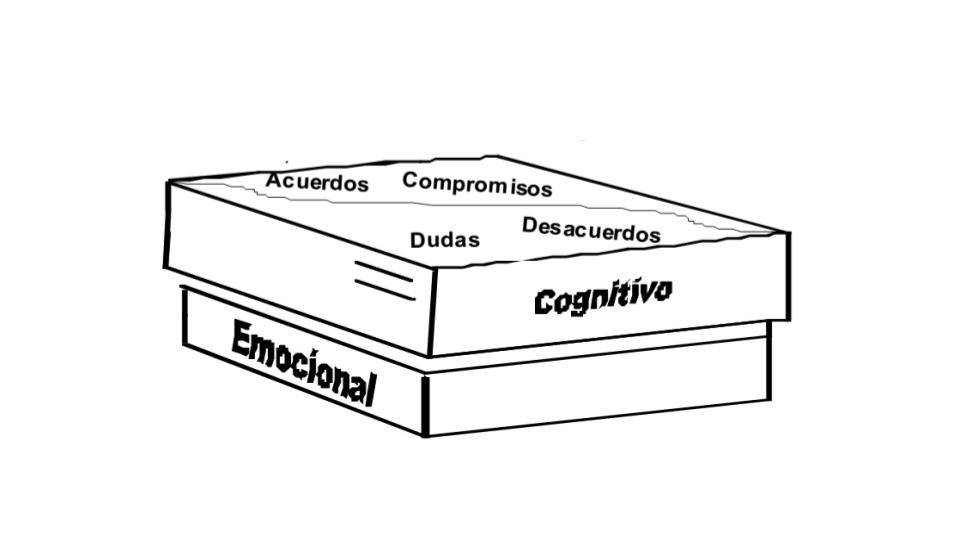
\includegraphics[width=0.7\linewidth]{/img2-1}
\caption{Plataforma del diálogo, tomado de (Leiva-Lobos, Antillanca y Ponce, 2008)} 
\label{img2-1}
\end{figure}

Aunque la dimensión emocional de los participantes en una conversación no se aborda en esta tesis; es preciso destacar que si no se generan las emociones adecuadas en una reunión, sencillamente el diálogo no ocurre. Además, es importante destacar que los componentes de la plataforma del diálogo mantienen y permiten llevar a una trayectoria histórica de la conversación que se puede seguir y gestionar.

Los elementos que componen la plataforma del diálogo y su descripción son los siguientes:

\begin{itemize}
	\item \textbf{Dudas (du):} Se plantea falta de información sobre un tema particular o no existe claridad sobre el problema, la oportunidad o las alternativas de solución. Esto crea incertidumbre en cómo continuar con el proyecto. Por ejemplo: “¿Qué tecnología es la más apropiada para este proyecto?”.
	\item \textbf{Desacuerdos (de):} Se presenta una contraposición entre puntos de vista sobre un tema o se detecta una brecha entre lo proyectado versus lo logrado. En ambos casos es necesario resolver el asunto para continuar el proyecto. Por ejemplo: “¡El proyecto será un éxito!,  yo no estaría tan confiado como tú”.
	\item \textbf{Compromiso (co):} Ciertos compromisos deben ser asumidos por personas específicas en fechas específicas para asegurarse que se realicen. Ni las reglas ni los acuerdos de coordinación colectivos logran ese efecto.  Por ejemplo: “Me comprometo que para la próxima reunión resolveré el problema del navegador chrome para funcione nuestro plug-in”.
	\item \textbf{Acuerdo (ac):} La coordinación grupal requiere acuerdos asumidos por todos. Si no son normas comunes o compromisos individuales se deben tratar como acuerdos de coordinación.  Por ejemplo: “Las reuniones diarias serán a las 12 pm”.

\end{itemize}

Si observamos los puntos anteriores nos podemos percatar que cada elemento conlleva una actividad y estas deben estar basadas en un parámetro común para todos pues el diálogo solo se puede generar si estamos dentro del mismo contexto conversacional \fullcite{RN34},  por favor observar la siguiente la figura \ref{img2-2}.

\begin{figure}[h]
\centering
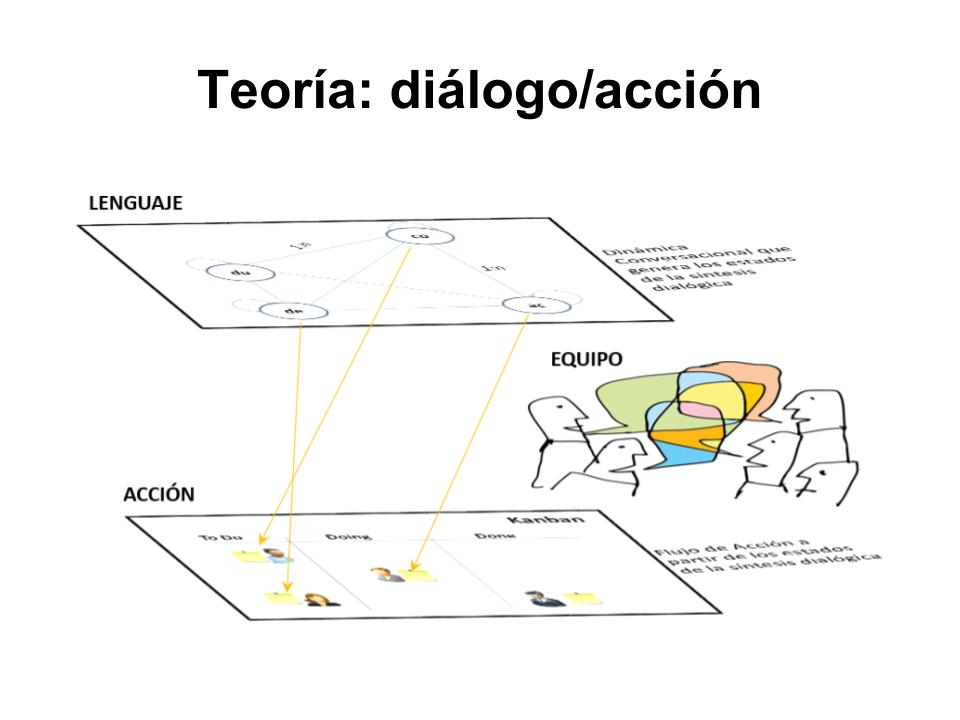
\includegraphics[width=0.7\linewidth]{/MetodoReunionesAgiles}
\caption{Articulación entre el plano del lenguaje y el plano de la acción que promociona el enfoque diálogo/acción, elaboración propia} 
\label{img2-2}
\end{figure}

Los acuerdos son declaraciones o reglas que fijan comportamientos humanos colectivos. Si son trascendentes para la demarcación del proyecto se llama “norma común”. Si esos acuerdos no fijan “una ley” permanente son consensos operativos se llaman “acuerdos de coordinación”. Por otro lado, para que se pase de los elementos del diálogo a la acción aparece un nuevo elemento denominado “tarea” (ta). Ahora, se identifican de manera más precisa estos tres elementos con las siguientes definiciones:

\begin{itemize}
	\item \textbf{Norma común:} La falta de normas, reglas o estándares comunes producen caos. Las normas y reglas comunes ordenan el trabajo. Estas reglas deben ser aceptadas colectivamente y consideradas leyes para operar en el futuro en el contexto del proyecto colectivo que se lleva a cabo. Por ejemplo: “Desde ahora en adelante usaremos solo metodologías Lean para proyectos pequeños”.
	\item \textbf{Acuerdos de coordinación:} Cuando no se trata de una regla o norma común y se precisa una coordinación en la acción se establecen por descarte este tipo de acuerdos. Por ejemplo, “Mañana a las 9 todos aquí”.
	\item \textbf{Tarea (ta):} Acción emprendida por una persona para lograr un objetivo. Aunque es obvio que un compromiso da lugar a una tarea. Resolver desacuerdos, resolver dudas, implementar normas, o la coordinación grupal dan origen a nuevas tareas. Luego se puede ir desde el conjunto (ac, de, du, co) a la tarea (ta). Un ejemplo de tarea es el siguiente: “Reparar el plug-in prometido en la reunión seis para las 12 am del jueves”.
\end{itemize}

Los elementos del dialog descritos, son representados por los iconos expuestos en imagen \ref{img2-3}

\begin{figure}[h]
\centering
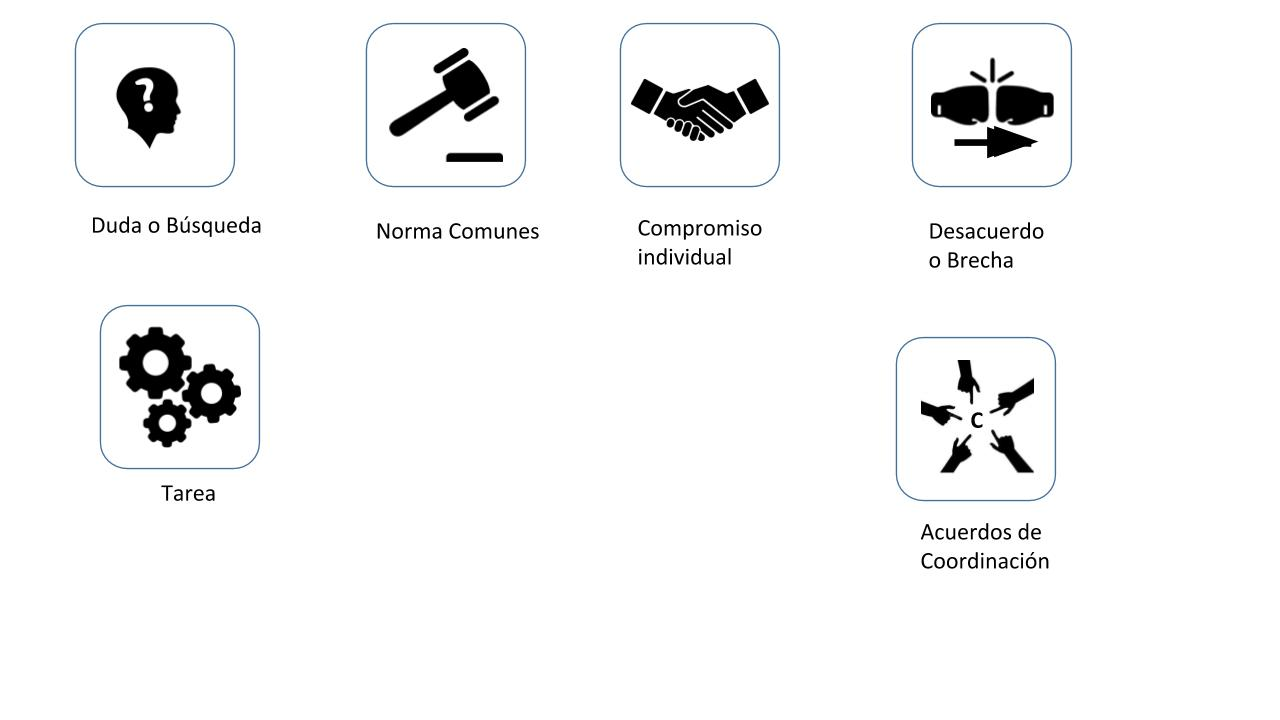
\includegraphics[width=0.7\linewidth]{/IconosDialogo-Accion}
\caption{Iconografía elementos del diálogo, elaboración propia} 
\label{img2-3}
\end{figure}

\subsection{ESTADO DEL ARTE}

Las reuniones y su efecto en las personas han sido analizadas por diferentes áreas del conocimiento: \textit{Knowledge Management, Dialogue, Collective Intelligence, Computer Supported Cooperative Work, Contested Collective Intelligence, meetingware}, por nombrar algunas; durante varias décadas han buscado que la comunicación, la coordinación, la cooperación sean parte integral de un flujo de trabajo colaborativo en reuniones del tipo \textit{co-located} síncrono y asíncrono, mediante el uso eficiente de la tecnología.

En 1970 Rittel y Kunz - citado por \fullcite{RN19} - publican \textit{Issue-Based Information System} (IBIS) un sistema para la captura de puntos esenciales en la discusión de problemas. Su notación se compone de: problemas (lo que se desea abordar), posiciones (las respuestas al problema) y argumentos (pros y contras de un problema), en 1988 Conklin y Begeman - citado por \fullcite{RN19} - adoptan el sistema para su uso en computadores, luego derivó a una variante para el mapeo de las conversaciones que se da en reuniones informales, para mejorar la inclusión de la discusión \fullcite{RN19}.

En 1986 Daft y Lengel - citado por \fullcite{RN21} - distinguen dos tipos de confusión que la gente puede tener con un elemento de discusión: la ambig\"uedad y la incertidumbre. Con esta distinción \fullcite{RN21} indican que las reuniones de decisión pueden considerarse como una composición de una parte divergente y una convergente. Proponen PRIME basado la notación de IBIS para el apoyo de reuniones de decisión y a su parte divergente de la discusión. Dicha parte que puede ser llamada “desacuerdo” relacionada con el cambio, en base a la teoría del diálogo propuesta el mismo año por \fullcite{RN24} donde postulan cuatro aspectos cognitivos que forman parte de la plataforma del diálogo, dos relacionados con la estabilidad: \textbf{acuerdo} al que se llega y \textbf{compromiso} que se toma (y quienes los toman); y dos relacionados con el cambio: \textbf{duda} que se genera al hablar de un tema y \textbf{desacuerdo} que se provoca cuando hay divergencia de opiniones. Esta teoría establece tres principios para el diálogo: apertura, continuidad y simetría. En particular, para ayudar a la continuidad del diálogo se conceptualiza un artefacto tangible denominado "Acta Dialógica" de allí el nombre del artefacto que se presenta en esta tesis D-Minute (\textit{Dialogic Minute}). A través de esta herramienta se pretende seguir la traza y el estado de los elementos que son parte de la plataforma del diálogo.

Chang, Liou Huang, Yu \& Shiah (1999) se mueven a la línea de \textit{co-located} asíncrono y proponen un sistema de minutas de conferencia basado en la \textit{World Wide Web} permitiendo tener hipervínculos de toda la información del proyecto, contener la memoria de la organización de este y que pueda ser heredada a nuevos participantes.

Volviendo a la línea \textit{co-located} síncrono \fullcite{RN37} presentan CollabMeet, un sistema de captura de información de reuniones basada en teléfono móvil, donde los participantes graban momentos importantes de la discusión, esto ayuda a minimizar las interrupciones y la distracción cuando la reunión es muy intensa. En una siguiente reunión pueden recurrir a la temática grabada en la reunión pasada para recuperar y re-situarse en el contexto del proyecto.

De Liddo \& Buckingham Shum (2010) exponen el modelo conceptual de Cohere, una plataforma hipermedia para investigación que permite explorar las nuevas ideas, apunta al concepto de inteligencia colectiva donde personas y grupos crean ideas en un entorno web. Ofrece seguimiento para las interpretaciones más allá si estas convergen o divergen entre sus participantes. Esto a su vez y en un área diferente pero no lejana se encuentra relacionado con la estabilidad o convergencia (acuerdo, compromiso) y el cambio o divergencia (desacuerdo, dudas) de la plataforma del diálogo propuesto en \fullcite{RN24}. Cohere además, se basa en IBIS para el mapeo de argumentos estructurados que se dan en las ideas expuestas por el grupo.

Bossel (2012) toma la teoría del diálogo de \fullcite{RN24} y genera un prototipo en papel de minuta que permita a un equipo reconectar y explorar la memoria colectiva del proyecto en base a reuniones periódicas, siguiendo la teoría del diálogo/acción.

En 2014 surgieron trabajos en la Universidad de Chile, que adoptaron el prototipo de minuta propuesto por \fullcite{RN14}, desarrollaron una aplicación web que facilita la continuidad y recuperación de los elementos del diálogo \fullcite{RN42} y que fue continuado por \fullcite{RN41} en su memoria de ingeniería civil en informática. Lamentablemente, ambos prototipos poseen demasiados problemas de usabilidad para ser considerados en una prueba de concepto robusta de las ideas de acta dialógica.

Por otra parte, sabemos que las reuniones son esenciales para coordinar y estructurar el trabajo, pero se estima que muchas de las herramientas desarrolladas en CSCW o groupware carecen de resultados en la práctica \fullcite{RN17} debido a que no son evaluadas de manera formal por los investigadores \fullcite{RN38}. Este punto es sumamente importante para la generación de un artefacto tecnológicos eficiente y usable y sobre todo válido.

Antunes \& Carrio (2003) proponen: Modelo de estructuras para reuniones, en el cual se identifican tres elementos fundamentales: (1) roles, abordando la diversidad de personas y actividades; (2) recursos, teniendo en cuenta la logística de la reunión y (3) proceso, dirigiéndose a la organización del conjunto de actividades.

En la misma línea Antunes \& Costa (2003) proponen: Perceived Value, un método para evaluar \textit{Meetingware} por medio de diferentes atributos respecto a una medida de costos y beneficios. Estos atributos son contribuciones que se dan por tres factores: individual, grupo y organización, básicamente porque el éxito o el fracaso depende de su combinación. Se organizan tres columnas, la primera se refiere a los roles, la segunda aborda el proceso de una reunión y la tercera para caracterizar el cumplimiento de los recursos donde la votación se limita a 0 para “no ayuda” y 1 “ayuda”, donde su “valor percibido” es calculado mediante una ecuación matemática, dicho valor debe ser mayor a la media (45). Siendo este resultado una medida para decidir si es válido continuar con la reunión. \fullcite{RN28} siguiendo una línea similar, describen el desarrollo y prueba de un instrumento para evaluar las reuniones por medio de un conjunto de factores de entrada, de proceso y resultado. Donde el primer paso de la evaluación es conocer el comportamiento en un marco de reuniones de proyecto y en segundo lugar medir los factores (evaluación, cuestionarios, etc), para determinar si el instrumento es confiable y útil para el apoyo a las reuniones.

Dhenesh, Sitnikova \& Slay (2012) para guiar la creación de herramientas, generan lecciones para el desarrollo de un sistema integrado que apoye las reuniones de trabajo y donde la adopción de la herramienta por los participantes sea inclusiva, debido a que muchas herramientas fallan en la práctica en incorporar esta característica.

\subsection{MARCO DE LA INVESTIGACIÓN DE MERCADO}

En este punto se formula cuál será el marco de investigación asociado a la innovación (la “i” chica en “I+D+i”) y desarrollo que guía este estudio. Se proponen las preguntas de investigación que se van a someter a análisis.

En la revisión bibliográfica realizada, las herramientas de \textit{meetingware} no poseen al menos las siguientes características que:

\begin{enumerate}[1.]
    \item Aplique elementos que sinteticen la convergencia y la divergencia de argumentos de manera explícita
    \item Exponga las tareas de forma visual.
    \item Permita recorrer las reuniones anteriores con flexibilidad y pertinencia.
    \item Permite editar los elementos del hilo argumental de la reunión y que son fruto de las discusiones al interior del equipo de desarrollo. En el caso de la teoría de diálogo/acción son los acuerdos, desacuerdos, dudas y compromisos.
\end{enumerate}

En base al estado del arte, se evidencia que existen herramientas que utilizan uno o alguno de los elementos del diálogo expuestos por \fullcite{RN24}. Sin embargo, los enfoques en los \textit{meetingware} desarrollados son distintos pero no alejados puesto que muchos conducen a una generación de diálogo. Esto propone las siguientes preguntas de investigación de mercado:

\begin{enumerate}[1.]
    \item ¿D-Minute expone los argumentos del diálogo y su seguimiento mejor que otras herramientas síncronas co-locadas de la investigación?
    \item ¿Qué ventaja competitiva posee D-Minute respecto a los productos comerciales existentes hoy día en el mercado?
\end{enumerate}

\subsection{RESUMEN}

El presente capítulo expone la revisión de la literatura que dan fundamento al desarrollo de esta tesis, situando en el contexto de \textit{meetingware} el trabajo realizar. Debido a que en esta línea de investigación es donde existe el mayor desarrollo de herramientas para el apoyo de reuniones, además de variados estudios que permiten medir la efectividad de las herramientas desarrolladas. 

En este trabajo y por medio de la plataforma del diálogo se busca determinar la efectividad que puede tener D-Minute -\textit{software} a desarrollar para la validación de la hipótesis- en comparación a otras herramientas del mercado. Es importante mencionar que D-Minute será la evolución del proyecto desarrollado en la Universidad de Chile por \fullcite{RN42} y la de \fullcite{RN41}.

Para este trabajo se va seleccionar herramientas del mercado que sirvan de apoyo a la reuniones de trabajo con el fin de establecer criterios de evaluación que permitan medir D-Minute con sus competidores es preciso leer el capítulo 3.

\section{MODELO LIVIANO DE NEGOCIO}

El objetivo de este capítulo es presentar el modelo de negocio de la solución desde una perspectiva de la innovación. En primera instancia se presenta lo que actualmente existe en el mercado asociado a los \textit{meetingware} en segundo lugar se identifica el marco de trabajo - desarrollado con la metodología \textit{Startup Lean} - donde se sitúa el producto a desarrollar. Pasando por el segmento de usuarios al cual está dirigido; luego, se presenta la propuesta de valor además de los canales del producto para ir finalizando con las ventajas competitivas del producto D-Minute.

\subsection{\textit{MEETINGWARE} COMERCIALES}

Antes de generar nuestro marco de trabajo es importante analizar las herramientas del mercado que poseen funcionalidades para el seguimiento de reuniones puesto que muchos productos de mercado abordan los temas que hemos analizado en capítulos anteriores. Lo anterior nos permite conocer a la competencia para establecer nuestra oferta de valor y ventaja competitiva.

A continuación se listan \textit{software} del mercado de más importancia\footnote{Los software de mercado fueron seleccionados desde \url{https://comparisons.financesonline.com/projectplace-software-vs-workep}}


\begin{enumerate}[1.]
    \item \textbf{Projectplace\footnote{\url{https://www.projectplace.com/}}}
    \begin{enumerate}[a]
	    \item \underline{Descripción:} Es una herramienta que permite a las empresas lograr sus objetivos por medio de la gestión de proyectos conjunta, facilitando la comunicación y colaboración del equipo. 
		\item \underline{Características:} Posee herramientas de planificación de proyectos, administración de tareas, gestión de documentos y gestión de reuniones. Permite realizar reuniones en línea, gestionar la cartera de proyectos y sus recursos, generar informes y notificaciones para realizar actividades de control. Es reconocido por sus excelentes medidas de seguridad. Comunicación en tiempo real a través de la fuente de conversación que fomenta la colaboración. Es compatible con aplicaciones móviles iOS y Android. Posee APIs que permite integración con otros \textit{software}.
	    \item \underline{Beneficios:} Facilita la colaboración al conocer las actividades principales, los hitos, las prioridades y proyectos del equipo independiente de donde se ubique cada miembro. Permite hacer seguimiento en línea de las tareas del equipo identificando alertas a tiempo cuando hay desvíos del foco. Permite que cada miembro tenga el control de su trabajo y los compromisos personales. Ofrece un punto de encuentro donde los empleados organizan reuniones en línea, comparten opiniones y archivos, teniendo todos acceso a la información necesaria. Una ventaja distintiva es que permite compartir archivos directamente desde sus cuentas de Google, Box o Dropbox. Posee el mecanismo de inicio de sesión único (Single Sign-On, SSO) que entrega un marco de identificación eficaz para evitar la pérdida de datos. En resumen es una única plataforma que centraliza todas las actividades relacionadas con la gestión de proyectos.
	    \item \underline{Precio:}  Existe sólo un plan a \$29.00 por usuario al mes, aunque para aquellos que deseen conocerla existe una versión de prueba gratis. La versión pagada incluye todas las características ya mencionadas. 
    \end{enumerate}	
    \item \textbf{Attentiv\footnote{\url{http://attentiv.com/}}}
    \begin{enumerate}[a]
	    \item \underline{Descripción:} Es una plataforma en la nube que busca mejorar la colaboración de los equipos y la toma de decisiones por medio de chat, votaciones, encuestas y comentarios. Es una herramienta que puede reducir los tiempos de reunión y ayudar a mejorar la cultura de la empresa. 
		\item \underline{Características:} Permite iniciar conversaciones en equipo, sea de forma anónima o no. También permite a los usuarios votar por los comentarios de los demás y filtrar los comentarios basados en estos votos ascendentes. Los usuarios pueden crear encuestas personalizadas para la respuesta del equipo y pueden organizar debates en diferentes grupos. 
	    \item \underline{Beneficios:} Con esta plataforma se puede obtener retroalimentación anónima o no y en línea. Permite destacar las buenas ideas que nacen de los equipos por medio de las votaciones. Este software fomenta tener menos reuniones, más efectivas y llegar a decisiones mejores y más informadas.
	    \item \underline{Precio:} Posee versión gratuita para grupos pequeños. Los grupos más grandes requieren una suscripción mensual. Versión gratis: hasta 10 usuarios, 1 GB de almacenamiento, encuestas y discusiones ilimitadas. Si requiere más capacidad tiene un costo de USD\$ 5 por usuario mensual, e incluye usuarios Ilimitados, almacenamiento de 20 GB, encuestas y discusiones ilimitadas. Por último, si aún se requiere mayor capacidad existe la versión a USD\$ 7 por usuarios mensual, que considera usuarios Ilimitados, almacenamiento de 20 GB, encuestas y discusiones ilimitadas.
    \end{enumerate}	    
    \item \textbf{Agreedo\footnote{\url{https://www.agreedo.com/es/index.html}}}
    \begin{enumerate}[a]
	    \item \underline{Descripción:} Es una aplicación orientada a la administración de reuniones. Su objetivo es capturar toda aquella información relevante que surge en cada reunión como lo son tareas, compromisos y decisiones. Permite compartir notas personales a otros miembros. 
		\item \underline{Características:} Programar reuniones y crear minutas, integración con distintos correos electrónicos (Outlook, Google Calendar, Lotus Notes, etc.). Seguridad del contenido basado en encriptación SSL. 
	    \item \underline{Beneficios:} Permite crear minutas estructuradas de reuniones, las cuales puedes compartir fácilmente. Permite hacer seguimiento de los compromisos de la reunión anterior, para aumentar la efectividad de éstas.
	    \item \underline{Precio:} La estructura de precios está compuesta por 3 versiones; gratis, premium y enterprise. La primera permite programar reuniones, crear minutas, sumar participantes y archivos de forma limitada. Integrarse con algún correo electrónico, además de poseer encriptación de contenido. La segunda tiene un costo de US\$ 7/mes (usuario único) o US\$ 60/mes (10 usuarios), y cuenta con las mismas funciones que la versión básica pero reuniones, participantes y archivos adjuntos ilimitados. Por último, existe la versión dirigida a empresas, la cual incluye las mismas características de la versión Premium más 100 MB de límite de tamaño de archivo adjunto.
    \end{enumerate}	    
    \item \textbf{Kairos\footnote{\url{https://kairos.lat/}}}
    \begin{enumerate}[a]
	    \item \underline{Descripción:} Es una plataforma orientada a eficientar el tiempo empleado en reuniones teniendo un propósito claro para lograr mayor productividad. Facilita el cumplimiento de tareas y entrega claridad sobre lo que se debe lograr por medio de su sistema de seguimiento y reportes.  
		\item \underline{Características:} Cuenta con agenda y dashboard donde se visualizan las próximas reuniones y tareas pendientes. Se pueden crear minutas rápidas y fáciles capturando acuerdos y compromisos con fecha de resolución, y además puedes asignarles responsables. Puedes enviar minutas por correo electrónico. Permite registrar avances de las tareas para realizar seguimiento. Está integrado con Google calendar para crear reuniones dentro y fuera de la plataforma, con Google Drive para adjuntar archivos y que todos manejen la misma información, y con Asana para dar seguimiento al cumplimiento de las tareas acordadas en tus reuniones.
	    \item \underline{Beneficios:} Esta plataforma tiene la capacidad de integrarse con las principales herramientas de administración de tareas; Asana, Google o Slack. Registra minutas, acuerdos y compromisos evitando malos entendidos. Posee herramientas de agenda y organización efectiva. Entrega reportería dirigida a la alta dirección sobre el desempeño del equipo. Organiza, registra y da seguimiento a acuerdos y tareas. Entrega visión clara sobre lo que se tiene que lograr y las tareas a realizar para cada integrante y a nivel global. 
	    \item \underline{Precio:} Existe la alternativa gratis que posee límite de hasta 3 usuarios. Por USD\$8 al mes permite interactuar hasta 25 usuarios, y en plan anual por USD\$7.
    \end{enumerate}	    
    \item \textbf{Evernote\footnote{\url{https://evernote.com/intl/es}}}    
    \begin{enumerate}[a]
	    \item \underline{Descripción:} Es una herramienta que permite capturar y compartir notas en cualquier formato (video, imagen, archivo de audio o notas escritas a mano), facilitando su búsqueda en cualquier dispositivo o lugar.
		\item \underline{Características:} Permite generar, editar y marcar texto, realizar bocetos y formas rápidamente. Cuenta con interfaz móvil y web. Permite almacenar notas, clips web, archivos e imágenes. Cuenta con geolocalización. Facilita la colaboración y creación compartiendo tus ideas con otras personas.  
	    \item \underline{Beneficios:} Permite almacenar distintos elementos dentro de una nota. Permite organizar reuniones rápidas y efectivas utilizando las notas almacenadas las cuales pueden transformarse fácilmente en presentaciones amigables.
	    \item \underline{Precio:} Existen 4 planes opcionales. El básico es sin costo e incluye poder compartir notas con acceso a 2 dispositivos. El Plus tiene un costo de US\$ 3.99/ mes o US\$ 34.99/año. Este tiene una capacidad mensual de 1GB en nuevas cargas, se sincroniza con todos tus dispositivos, permite buscar texto dentro de las imágenes, puedes compartir notas con otras personas, incluye soporte y puedes acceder sin conexión. El Premium tiene un  costo de USD\$ 7.99/mes o US\$ 69.99/año. Permite 10 GB de nuevas cargas por mes, todas las funciones del Plus más buscar texto y editar PDF. La versión para empresas tiene un costo por usuario al mes de US\$ 14.99, incluye 20 GB de nuevas cargas al mes más 2 GB por usuario. Adicional a las características de la versión Premium cuenta con inicio de sesión único y administración central de usuarios.
    \end{enumerate}	    
    \item \textbf{Workep\footnote{\url{https://workep.com/es/es.html}}}    
    \begin{enumerate}[a]
	    \item \underline{Descripción:} Es una plataforma para la gestión de proyectos que permite a los equipos trabajar de forma conjunta sin importar la locación de sus miembros, desarrollada especialmente para trabajar con la Suite Google.  
		\item \underline{Características:} Administración de tareas, búsqueda general de proyectos, tareas y contactos, manejo de gantt, integración con aplicaciones de Google, notificaciones de correo electrónico inteligente.
	    \item \underline{Beneficios:} Ayuda a que los equipos de proyecto permanezcan coordinados durante la vida del proyecto. Posee gráficas detalladas que dan claridad sobre los proyectos y su progreso. Organiza y centraliza toda los archivos y otros materiales de contenido. Al ser una plataforma que de forma nativa está diseñada para integrarse a las herramientas Google, facilita su adopción por la familiaridad de éstas para las personas y empresas. Facilita la comunicación y trabajo en equipo en todo lugar y momento con sus herramientas; Calendar, Drive, Hangouts, entre otras. 
	    \item \underline{Precio:} Existe la versión gratis que incluye la plataforma básica; tareas, proyectos y archivos ilimitados, hasta 10 miembros del equipo, solo 1 equipo, integraciones con G Suite. Otra opción es la versión escalable, con un costo mensual de \$2.99 por usuario. Esta incluye las mismas características de la versión gratis, pero no restringe el número de equipos ni miembros. Además ofrece roles y soporte prioritario. Finalmente existe la opción Crecimiento la cual contiene las mismas características de la versión antes mencionada, sin embargo adiciona plantillas de proyecto, dependencias de tareas, gantt avanzado, Rastreador de tiempo, búsqueda universal y marca personalizada. Su costo es de \$4.99/usuario por mes.
    \end{enumerate}	      
\end{enumerate}

\subsection{MARCO DE LA INNOVACIÓN}

Para generar el marco de la innovación del software D-Minute se utilizó la metodología \textit{Lean Startup} desarrollada por Eric Ries \fullcite{RN29}, el cual es una guía para: establecer el segmento de clientes que tendrá foco el proyecto, sus oportunidades respecto al mercado, los flujos de ingreso que podría alcanzar la plataforma para el retorno de la inversión y su propuesta de valor diferenciada. Estos puntos son relevantes para establecer los canales de difusión, la estructura de costos necesaria para iniciar el desarrollo y la ventaja competitiva respecto al mercado. Lo anterior nos va permitir generar el lienzo del modelo de negocio para D-Minute.

\subsubsection{Segmento de destinatarios}

La mayoría de empresas hoy en día requieren de reuniones de trabajo para el seguimiento de tareas, por tanto el segmento importante que requiera de un sistema de minutas es: proveedores de \textit{software} a medida, servicios de consultoría, bancos, servicios públicos, empresas de obra gruesa y ONGs.

\subsubsection{Oportunidades}

Como hemos detectado en CAPÍTULO 1, CAPÍTULO 2 y en base a lo que hemos recogido de los \textit{meetingware} comerciales. Se observan funcionalidades que deben estar presente en programas que coordinan equipos de trabajo, hacen seguimiento a tareas y compromisos, definen alcances y funcionalidades, comprometen recursos entre otras actividades. Dichas oportunidades son:

\begin{enumerate}[1.]
	\item Debe incorporar el concepto de “proyecto” como el conjunto de reuniones
	\item Recorrer las reuniones anteriores con flexibilidad y pertinencia. 
	\item Aplicar elementos que sinteticen la convergencia y la divergencia de argumentos de manera explícita
	\item Permitir editar los elementos del hilo argumental de la reunión y que son fruto de las discusiones al interior del equipo de desarrollo. En el caso de la teoría de diálogo/acción son los acuerdos, desacuerdos, dudas y compromisos.
	\item Registrar tareas que nacen de los compromisos individuales de forma automática y de una manera visual para seguimiento.
\end{enumerate}

\subsubsection{Flujos de ingreso}

Toda solución requiere conocer la forma que se recupera la inversión, dado los costos que existen por herramientas de este tipo se detecta que los flujos de ingreso se pueden dar por: 

\begin{enumerate}[1.]
	\item Modelo de suscripción
	\item Arriendo del servicio por reunión - Flat Rate 
	\item Publicidad en costados - Uso financiado por publicidad
	\item Arriendo de la plataforma - \textit{White Label}
\end{enumerate}

Lo anterior considerando que el producto pasa por generación, adopción y mejora continua como ciclo de vida de costo.

\subsubsection{Propuesta de valor}

Generar reuniones efectivas es el gran desafío que se presenta en el área del \textit{meetingware} debido a los costos directos e indirectos que se generan por esta instancia. La propuesta de valor se enfoca en criterios que devuelvan la efectividad a las reuniones en los equipos creativos y agilizando las reuniones de proyecto con una síntesis del diálogo.

Los criterios son los siguientes:

\begin{enumerate}[1.]
	\item \textbf{Usable}, en otras palabras se espera que todas sus componentes para manejar sets de reuniones de un proyecto exhiba usabilidad.
	\item \textbf{Trazable}, es decir, el sistema debe tener una forma visual de administrar las relaciones causales entre los elementos dialógicos que se dan en las reuniones: acuerdos, compromisos, dudas y desacuerdos.
	\item \textbf{Buscable}; quiere decir que siempre habrá filtros para encontrar lo que se busca de las reuniones.
	\item \textbf{Accionable}, que por medio de un tablero Kanban de reuniones se generen tareas para un elemento del dialógico, el compromiso individual.
\end{enumerate}


\subsubsection{Canales}

Se identifica que el medio por el que se hará llegar la propuesta de valor al segmento de clientes, se da por regalar el producto en una ONGs para “envirar” el ambiente empresarial, cuentas oficiales de D-Minute (Instagram, youtube, twitter y facebook), conversación con oficina de proyecto (PMO) empresariales y oferta del producto por web diferenciada por tamaño de empresa.

\subsubsection{Recursos claves}

Con el fin de garantizar una implementación correcta del producto es necesario conocer qué tipo de recursos son claves para el éxito, en este caso hemos detectado:

\begin{enumerate}[1.]
	\item Servicio cloud con escalamiento dinámico
	\item Desarrollador \textit{fullstack} en el uso de micro arquitectura
	\item Notebook de desarrollo
	\item Servidor de Dominio 
\end{enumerate}

\subsubsection{Estructura de costos}

Para operar el modelo de negocio se debe incurrir en costos que permitan operar, por tanto la estructura debe considerar: costos de creación y entrega de valor, relaciones con cliente y generación de ingresos. 

Las siguientes preguntas definen la estructura de costos:

\begin{enumerate}[1.]
	\item ¿Cuáles son los costos más importantes para mantener el modelo de negocio? 
	
	\textbf{R:} Diseño UX, Servidor de dominio, Programador \textit{fullstack} y \textit{Cloud Service}.
	\item ¿Cuáles son los recursos claves más caros? 
	
	\textbf{R:} \textit{Cloud Service} y Programador \textit{fullstack}
	\item ¿Cuáles son las actividades claves más caras? 

	\textbf{R:} Programación 

	\item ¿Qué actividades claves están realizando nuestros socios? 
	
	\textbf{R:} Programación
\end{enumerate}

\subsubsection{Ventaja competitiva como emprendimiento}

Esta parte se pone como frases de marketing y en este caso son las siguientes: 

\begin{enumerate}[1.]
	\item Conocemos de \textit{meetingware}, management y comunicación efectiva.
	\item Nuestro trabajo se basa en un paper sobre la teoría del diálogo y en una tesis de Magíster que prueba la efectividad del método dialógico.
	\item Soporte de \textit{couching} de comunicación efectiva en empresas
\end{enumerate}

\subsubsection{Lienzo D-Minute}

El lienzo Canvas es el resumen de nuestro temas abordados y representa nuestro modelo de negocio para nuestro mínimo producto viable (en adelante MVP, del inglés \textit{Minimum Viable Product}), representado en imagen \ref{img3-1}.

\begin{figure}[h]
\centering
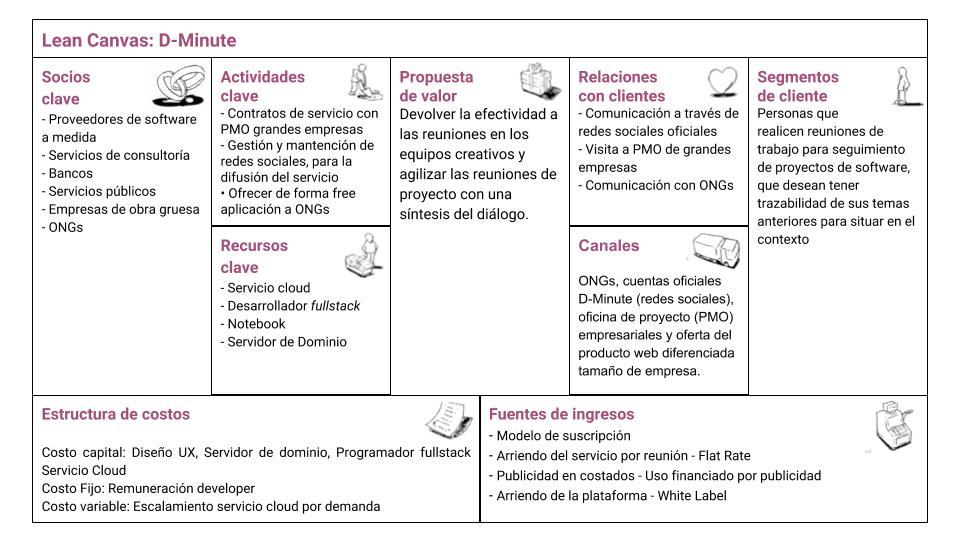
\includegraphics[width=1\linewidth]{/LeanCanvas}
\caption{Lienzo Canvas D-Minute, tomado de Lean Canvas y elaboración propia} 
\label{img3-1}
\end{figure}

\subsection{\textit{BENCHMARKING}}

El \textit{benchmarking}\footnote{Benchmarking para más información acerca de esto ver los siguiente enlaces \url{https://www.economiasimple.net/glosario/benchmarking} y \url{https://es.wikipedia.org/wiki/Benchmarking} } aplicado a D-Minute corresponde a la categoría funcional pues nos hemos orientado a competidores directos como indirectos - un ejemplo de competidor indirecto es Evernote dado que no es un software de reuniones pero es de uso frecuente en ellas - con la finalidad de responder los criterios de evaluación de cada productos. Cada criterio está basado en la literatura expuesta en el marco conceptual del CAPÍTULO 2, el cual menciona que es lo mínimo que debe poseer un sistema de reuniones para ser un apoyo y no al revés, ver imagen \ref{img3-2}.

\begin{figure}[h]
\centering
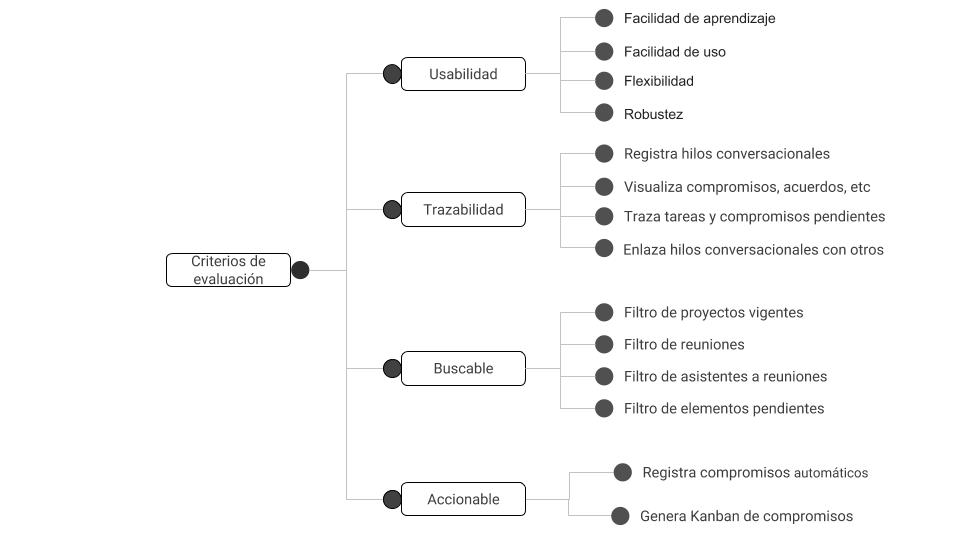
\includegraphics[width=1\linewidth]{/CriteriosBenchmark}
\caption{Criterios evaluados para un \textit{meetingware}, elaboración propia} 
\label{img3-2}
\end{figure}

Se ha definido cuatro pilares de evaluación de nivel macro pues son la base para un gestor de reuniones y por cada pilar se establecen subcriterios de evaluación que nos permiten identificar si los sistemas poseen al menos una de las funcionalidades del pilar. Por último, para determinar cuan efectiva es una herramienta se asigna un porcentaje de relevancia a cada uno de los pilares y sub-pilares, estos valores fueron obtenidos de encuestas realizadas a gestores de proyecto que a diario se ven enfrentados a reuniones de trabajo, ver anexo A.  Los datos estan representadas en las tablas \ref{tab:usable} - \ref{tab:trazable} - \ref{tab:buscable} - \ref{tab:accionable} que contienen: Item\footnote{Corresponde a la descripción evaluada del criterio}, Porcentaje Nota Obtenida\footnote{Nota Obtenida: corresponde a la suma de los promedios obtenidos por la cantidad de personas encuestadas}, Q. Respuesta\footnote{Q de Respuesta: corresponde al número de personas que respondió el sub criterio.}.

\begin{table}[!h]
\centering
\caption{Resultado criterio Usable, elaboración propia}
\label{tab:usable}
\begin{tabular}{|l|r|r|}
\hline
\multicolumn{3}{|c|}{Criterio Usable} \\ \hline
\multicolumn{1}{|c|}{Ítem} & \multicolumn{1}{c|}{Porcentaje Nota Obtenida} & \multicolumn{1}{c|}{Q. Respuesta} \\ \hline
Facilidad de aprendizaje & 33.3 & 7 \\ \hline
Facilidad de uso & 85,7 & 18 \\ \hline
Flexibilidad & 47,6 & 10 \\ \hline
Robustez & 52,4 & 11 \\ \hline
\end{tabular}
\end{table}

\begin{table}[!h]
\centering
\caption{Resultado criterio Trazable, elaboración propia}
\label{tab:trazable}
\begin{tabular}{|l|r|r|}
\hline
\multicolumn{3}{|c|}{Criterio Trazable} \\ \hline
\multicolumn{1}{|c|}{Ítem} & \multicolumn{1}{c|}{Porcentaje Nota Obtenida} & \multicolumn{1}{c|}{Q. Respuesta} \\ \hline
Registra hilos conversacionales & 81 & 17 \\ \hline
Traza tareas y compromisos pendientes & 66,7 & 14 \\ \hline
Enlaza hilos conversacionales con otros & 38,1 & 8 \\ \hline
\end{tabular}
\end{table}

\begin{table}[!h]
\centering
\caption{Resultado criterio Buscable, elaboración propia}
\label{tab:buscable}
\begin{tabular}{|l|r|r|}
\hline
\multicolumn{3}{|c|}{Criterio Buscable} \\ \hline
\multicolumn{1}{|c|}{Ítem} & \multicolumn{1}{c|}{Porcentaje Nota Obtenida} & \multicolumn{1}{c|}{Q. Respuesta} \\ \hline
Filtro de proyectos vigentes & 71,4 & 15 \\ \hline
Filtro de reuniones & 85,7 & 18 \\ \hline
Filtro de asistentes a reuniones & 47,6 & 10 \\ \hline
Filtro de elementos pendientes & 71,4 & 15 \\ \hline
\end{tabular}
\end{table}

\begin{table}[!h]
\centering
\caption{Resultado criterio Accionable, elaboración propia}
\label{tab:accionable}
\begin{tabular}{|l|r|r|}
\hline
\multicolumn{3}{|c|}{Criterio Accionable} \\ \hline
\multicolumn{1}{|c|}{Ítem} & \multicolumn{1}{c|}{Porcentaje Nota Obtenida} & \multicolumn{1}{c|}{Q. Respuesta} \\ \hline
Registra compromisos automáticos & 52,4 & 11 \\ \hline
Genera Kanban de compromisos & 81 & 17 \\ \hline
\end{tabular}
\end{table}

\begin{table}[!h]
\centering
\caption{Resultado encuesta de criterios, elaboración propia}
\label{tab:resultado}
\begin{tabular}{|l|r|r|}
\hline
\multicolumn{1}{|c|}{Criterio} & \multicolumn{1}{c|}{Nota Promedio} & \multicolumn{1}{c|}{Nota final} \\ \hline
Usable & 81 & 17 \\ \hline
Trazable & 81 & 17 \\ \hline
Buscable & 52,4 & 11 \\ \hline
Accionable & 81 & 17 \\ \hline
\end{tabular}
\end{table}

De los datos capturados se calculó el promedio de la nota obtenida por criterio con el fin de establecer cuál de ellos posee una mayor relevancia para los encuestados y a su vez determinar el porcentaje final de cada criterio en escala de 1 a 100, en términos porcentuales, ver imagen \ref{img3-3}.


\begin{figure}[!h]
\centering
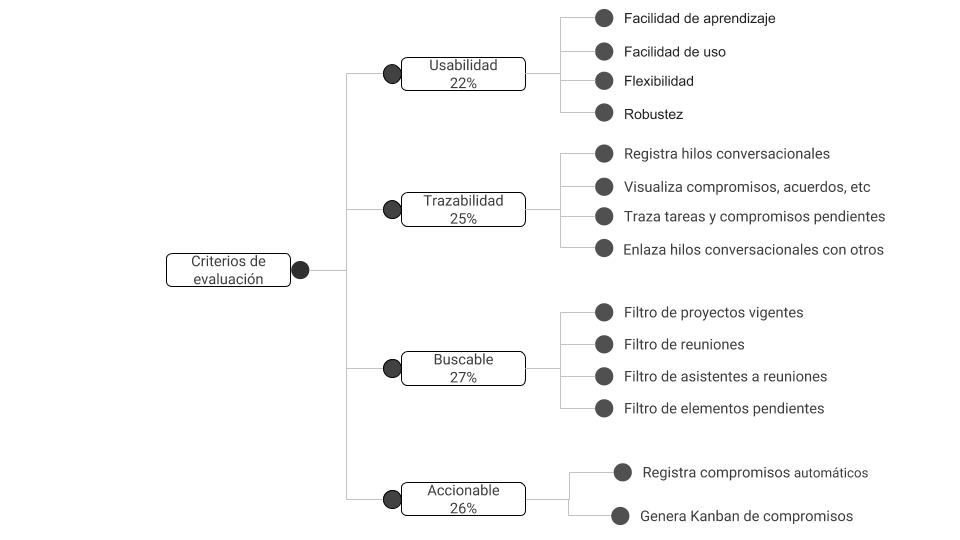
\includegraphics[width=1\linewidth]{/CriteriosBenchmarkPorcentaje}
\caption{Resultado criterio de evaluación \textit{meetingware}, elaboración propia} 
\label{img3-3}
\end{figure}

Para determinar la nota final de cada criterio con la Ecuación 1, se utilizó el promedio de cada uno - ver tabla \ref{tab:resultado} - sobre la suma de los promedios, determinando de esta forma la importancia relativa en términos porcentuales.

Si bien los datos muestran que todos los sistemas poseen a lo menos tres de cuatro pilares. El pilar de trazabilidad es uno de los más relevantes en el contexto de reuniones el cual coindice con lo expone por: \fullcite{RN24}, \fullcite{RN15}, \fullcite{RN37}, \fullcite{RN16} entre otros mencionados en el CAPÍTULO 2 sección 2.3, debido a que trabajar con una síntesis dialógica mejora y sitúa en contexto a los participantes de una reunión. D-Minute posee los cuatro pilares pues y uno de los focos es la síntesis del diálogo expuesta por \fullcite{RN24}, donde se centra este software y trabajo, ver resultado en tabla \ref{tab:resultadoevaluacion}.

\begin{table}[!h]
\centering
\caption{Resultado evaluación de \textit{meetingware}, elaboración propia}
\label{tab:resultadoevaluacion}
\resizebox{15cm}{!} {
\begin{tabular}{|l|l|c|c|c|c|c|c|c|}
\hline
\multicolumn{1}{|c|}{Pilar} & \multicolumn{1}{c|}{Criterio} & D-Minute & Projectplace & Attentiv & Agreedo & Kairos & Evernote & Workep \\ \hline
\multicolumn{1}{|c|}{\multirow{4}{*}{Usabilidad}} & Facilidad de aprendizaje & x &  & x &  & x & x & x \\ \cline{2-9} 
\multicolumn{1}{|c|}{} & Facilidad de uso & x &  & x & x & x & x & x \\ \cline{2-9} 
\multicolumn{1}{|c|}{} & Flexibilidad & x & x &  &  &  & x & x \\ \cline{2-9} 
\multicolumn{1}{|c|}{} & Robustez & x & x &  &  & x & x & x \\ \hline
\multirow{4}{*}{Trazabilidad} & Registra elementos de diálogo & x & x &  & x & x &  &  \\ \cline{2-9} 
 & Visualiza elementos de diálogo & x & x &  & x & x &  &  \\ \cline{2-9} 
 & Traza elementos de diálogo pendientes & x & x &  &  & x &  &  \\ \cline{2-9} 
 & Enlaza elementos de diálogo & x &  &  &  &  &  &  \\ \hline
\multirow{4}{*}{Buscable} & Filtro de proyectos vigentes & x & x &  &  &  & x & x \\ \cline{2-9} 
 & Filtro de reuniones & x &  &  & x &  & x & x \\ \cline{2-9} 
 & Filtro de asistentes a reuniones & x &  &  &  &  & x &  \\ \cline{2-9} 
 & Filtro de elementos pendientes & x &  &  &  &  &  &  \\ \hline
\multirow{2}{*}{Accionable} & Registra compromisos automáticos & x &  &  &  &  &  & x \\ \cline{2-9} 
 & Genera Kanban de compromisos &  &  &  &  & x &  &  \\ \hline
\end{tabular}
}
\end{table}

En consecuencia, con los criterios de comparación establecidos y en igualdad de condiciones tenemos una clara ventaja de D-Minute en relación a todas las herramienta que se analizaron en esta tesis. 88\% es un número lo suficientemente significativo para demostrar la ventaja de la herramienta que se propone en este tesis de magister, el resultado se puede ver en la tabla \ref{tab:evaluacionfinal}.

\begin{table}[!h]
\centering
\caption{Cálculo del peso de los \textit{meetingware} evaluados, elaboración propia}
\label{tab:evaluacionfinal}
\resizebox{15cm}{!} {
\begin{tabular}{cl|r|r|r|r|r|r|r|}
\cline{3-9}
\multicolumn{1}{l}{} &  & \multicolumn{7}{c|}{\textbf{Meetingware}} \\ \cline{3-9} 
\multicolumn{1}{l}{} & \multicolumn{1}{c|}{} & \multicolumn{1}{c|}{D-Minute} & \multicolumn{1}{c|}{Projectplace} & \multicolumn{1}{c|}{Attentiv} & \multicolumn{1}{c|}{Agreedo} & \multicolumn{1}{c|}{Kairos} & \multicolumn{1}{c|}{Evernote} & \multicolumn{1}{c|}{Workep} \\ \hline
\multicolumn{1}{|c|}{\multirow{4}{*}{\textbf{Porcentaje Pilar}}} & Usabilidad (22\%) & 22 & 11 & 11 & 5,5 & 16,5 & 22 & 22 \\ \cline{2-9} 
\multicolumn{1}{|c|}{} & Trazabilidad (25\%) & 24 & 18 & 0 & 12 & 18 & 0 & 0 \\ \cline{2-9} 
\multicolumn{1}{|c|}{} & Buscable (27\%) & 28 & 7 & 0 & 7 & 0 & 21 & 14 \\ \cline{2-9} 
\multicolumn{1}{|c|}{} & Accionable (26) & 13,5 & 0 & 0 & 0 & 0 & 0 & 13,5 \\ \hline
\multicolumn{2}{|r|}{\textbf{Totales}} & \textbf{88\%} & \textbf{36\%} & \textbf{11\%} & \textbf{25\%} & \textbf{35\%} & \textbf{43\%} & \textbf{50\%} \\ \hline
\end{tabular}

}
\end{table}


\subsection{RESUMEN}

El presente capítulo expone los diferentes software de mercado que permiten hacer seguimiento a reuniones de proyecto. Por cada \textit{software} se analizaron las características sus beneficios, los factores relevantes de cada herramienta y por último su valor de mercado. Esto nos genera una fuente valiosa de información que se hace relevante a la hora conocer si nuestro MVP es un producto viable, usable y competitivo. 

Dado el análisis anterior, en la segunda parte del capítulo fue generado el marco de innovación del \textit{software} D-Minute representado en el lienzo “Lean Canvas” de la aplicación D-Minute.

Para concluir se realizó un \textit{benchmarking} de los diferentes sistemas revisados y se aplicó un cuadro comparativo de los criterios de evaluación analizados en el capítulo uno y dos, para determinar cómo se sitúa D-Minute en el mercado.

En los próximos capítulos se va presentar el desarrollo de la solución y en forma posterior establecer los criterios de evaluación que nos permitan validar las preguntas de investigación más allá del mercado.


\section{DESARROLLO DE LA APLICACIÓN}

El objetivo de este capítulo es presentar el desarrollo de la aplicación pasando por el \textit{framework} metodológico asociado, la definición de las épicas con sus respectivas historias de usuario para finalmente definir la cantidad de sprint necesarias para obtener el mínimo producto viable de la aplicación. En el mismo capítulo se presenta como se conformó el equipo y estructura utilizando la metodología Scrum. 

\subsection{\textit{FRAMEWORK} AGILE}

Hoy en día existen muchos \textit{framework} para el desarrollo de \textit{software}, sin embargo para la construcción de la aplicación D-Minute hemos seleccionado algunos de los artefactos y ritos de Scrum \fullcite{RN33} dada sus ventajas y familiarización que tiene el team de desarrollo. Es importante mencionar que Scrum ver imagen \ref{img4-1} es uno de los framework más utilizados en la industria del \textit{software} a nivel mundial\footnote{Tomado de: \url{https://www.forbes.com/sites/stevedenning/2015/07/23/the-worlds-most-popular-innovation-engine/\#25f09da7c769}}, algunas de sus ventajas\footnote{Tomado de: \url{https://alfatecsistemas.es/los-10-beneficios-la-metodologia-scrum/} y \url{http://scrumguides.org/docs/scrumguide/v2017/2017-Scrum-Guide-US.pdf\#zoom=100}} son las siguientes:

\begin{enumerate}[1.]
    \item Fomenta la motivación y el compromiso del equipo 
    \item Provoca una mayor productividad al eliminar la burocracia.
    \item La organización horizontal promueve la autonomía y la auto-organización.
    \item El desglose del trabajo favorece a una mayor flexibilidad a los cambios. 
    \item Este trabajo intensificado conlleva una alta predicción de tiempos puesto que se conoce la velocidad y rendimiento del equipo.
    \item Dominar estos rasgos del equipo de trabajo reduce los riesgos al conocer las funcionalidades de cada rol y la velocidad a la que avanza el proyecto.
    \item La capacidad de flexibilidad y la reducción de riesgos permiten cumplir las expectativas del cliente.
    \item También, reduce el Time to Market: el cliente puede empezar las funcionalidades principales del proyecto antes de que este esté acabado.
    \item El método de trabajo y la revisión continua produce una mayor calidad del \textit{software}.

\end{enumerate}

\begin{figure}[h]
\centering
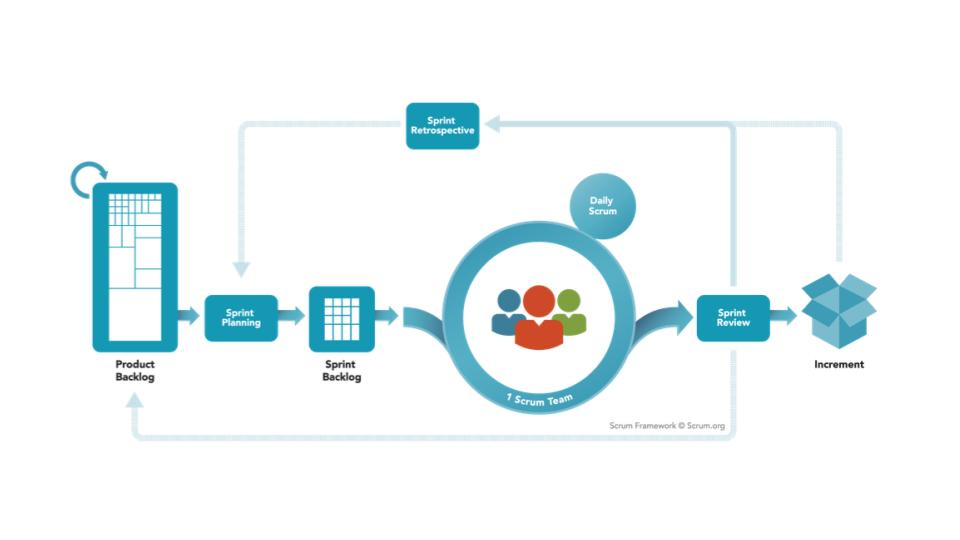
\includegraphics[width=1\linewidth]{/scrum}
\caption{Framework Scrum; tomado de Scrum.org} 
\label{img4-1}
\end{figure}

Si bien el \textit{framework} es una guía para la forma de abordar el desarrollo de la mejor manera, se requiere una herramienta para realizar la gestión respectiva del proyecto, para este caso se utilizó la plataforma online TAIGA\footnote{TAIGA: aplicación para seguimiento de proyectos ágiles, ver \url{https://taiga.io/}} ver imagen \ref{img4-2}

\begin{figure}[!h]
\centering

\includegraphics[width=12cm]{/taiga}
\caption{Vista principal de la plataforma para seguimiento proyecto; tomada de Taiga.io} 
\label{img4-2}
\end{figure}

\subsection{\textit{TEAM} DESARROLLO}

Scrum recomienda que un equipo “(...) debe ser pequeño como para permanecer ágil y lo suficientemente grande como para completar una cantidad significativa de trabajo” \fullcite{RN33}, pero no se recomienda más de nueve personas, dado lo anterior el equipo se conforma por cinco personas con diferentes roles, ver imagen \ref{img4-3}

\begin{figure}[!h]
\centering
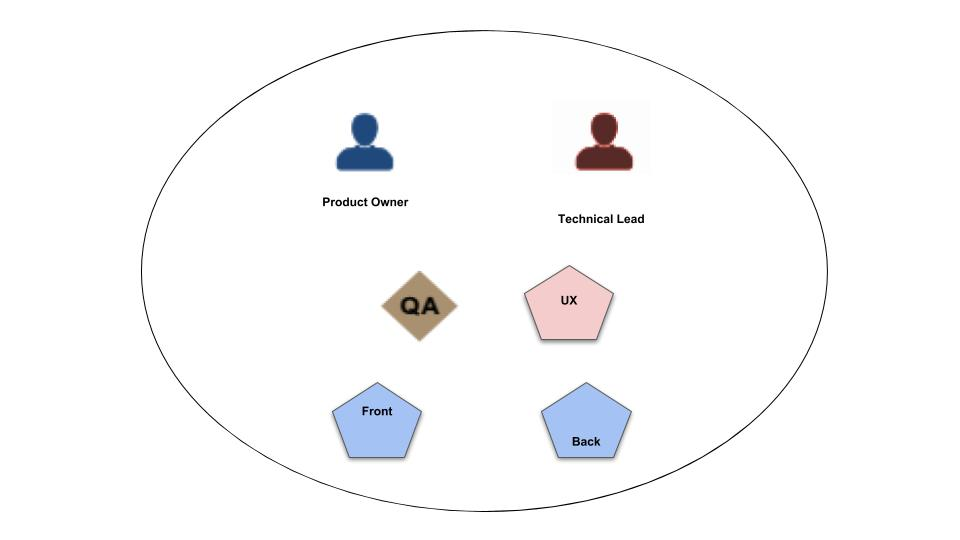
\includegraphics[width=10cm]{/equipo}
\caption{Estructura de equipo desarrollo y roles incorporados; elaboración propia} 
\label{img4-3}
\end{figure}

Si bien existe un equipo multidisciplinario, es importante indicar que a cada una de las personas individualizadas se les presentó el proyecto invitándolos a participar de esta iniciativa sin compromiso y sin un pago establecido. Los roles asumidos son los siguientes:

\begin{enumerate}[1.]
    \item Product Owner: Edmundo P. Leiva-Lobos (profesor guía)
    \item Technical Lead: Oliver Hidalgo (tesista)
    \item QA: Michele Fuenzalida
    \item Front: Francisco Gonzalez 
    \item Back: Andres Perez
    \item UX: Valentina Reyes
\end{enumerate}

\subsection{ÉPICAS}

Una epica es un concepto de agrupación  de funcionalidades que forma un macro requerimiento de negocio, esta puede contener muchas historias de usuarios que el equipo debe ir descomponiendo para lograr el desarrollo a un nivel de 80/20\footnote{ El concepto 80/20 indica que del 100\% de un producto sólo se ocupa el 20\% y el 80\% restante es desperdicio. Esto no es otra cosa que la aplicación de la famosa Ley de Pareto}. Para el proyecto en cuestión se identificaron los macro conceptos necesarios para obtener un MVP\footnote{MVP = Mínimo Producto Viable}, estas épicas se detallan y se muestran en figura \ref{img4-4}:

\begin{enumerate}[1.]
   \item Evolución UX: Corresponde a la línea gráfica desarrollada en la aplicación
   \item Deuda Técnica: Corresponde a las HDU técnicas que surgieron en el desarrollo de la aplicación
   \item Generación Acta: Corresponde a la funcionalidad completa de crear un acta
   \item Seguimiento de Tareas: Corresponde a la funcionalidad del seguimiento de los elementos del diálogo
   \item Trazabilidad elementos del diálogo: Corresponde al seguimiento de los elementos del diálogo una vez creados
\end{enumerate}

\begin{figure}[!h]
\centering
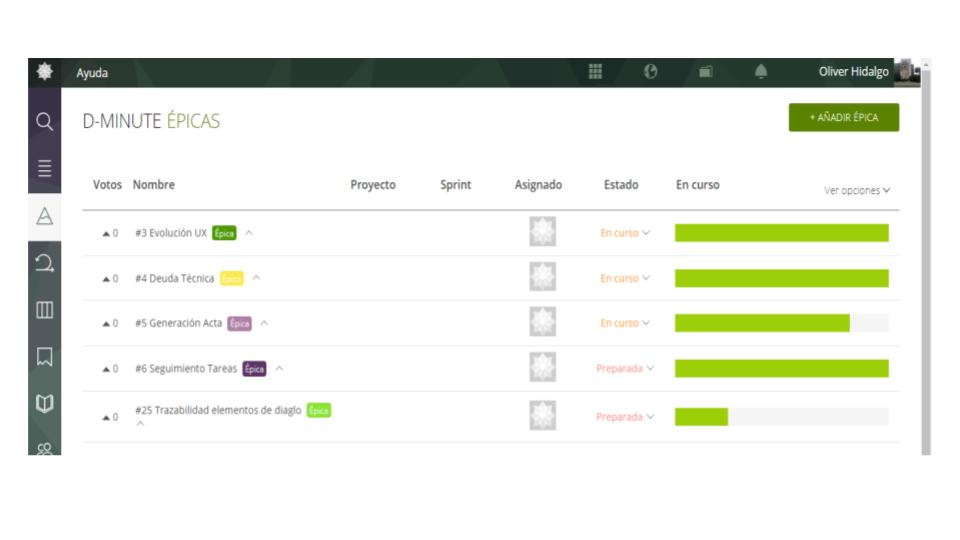
\includegraphics[width=12cm]{/epicas}
\caption{Épicas D-Minute; elaboración propia} 
\label{img4-4}
\end{figure}

\subsection{\textit{RELEASE MAP}}

Un \textit{release map} representa la visión general del proyecto dado los plazos fijos que se posee para llevar a cabo el desarrollo. Importante mencionar que el equipo puede ir tomando historias de usuario de diferentes épicas pues el objetivo es ir generando un software funcionando en cada iteración y obtener feedback temprano del cliente, a continuación se presentan las épicas - en imagen \ref{img4-5} - del producto que fueron planificadas al inicio del desarrollo:

\begin{figure}[!h]
\centering
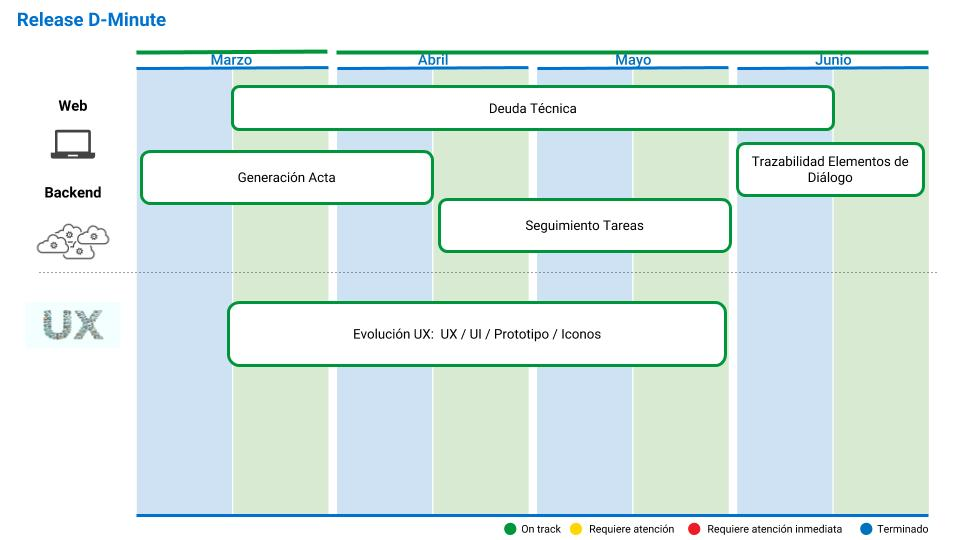
\includegraphics[width=12cm]{/releasemap}
\caption{Release Map D-Minute; elaboración propia} 
\label{img4-5}
\end{figure}

\subsubsection{Duración de \textit{Sprint}}

Dado el análisis del equipo y los tiempos para llevar a cabo este desarrollo se definió que cada \textit{sprint} tendría una duración fija de dos semanas para permitir conocer la velocidad del equipo e ir ajustando en cada iteración. 	

\subsubsection{Cantidad de \textit{Sprint}}

La cantidad de \textit{sprint} está dada por el tiempo que se posee para el desarrollo del producto, para este caso se generaron ocho \textit{sprint}.

\subsubsection{Versión UX/UI}

D-Minute, es una aplicación que deriva de otra llamada meetingviewer que fue desarrollada por una alumna de ingeniería de la Universidad de Chile, como se menciona en el CAPÍTULO 1, que a su vez nace del prototipo desarrollado por Bossel en 2012. Si bien es un \textit{software} existente, no es una versión estable y lista de cara a clientes pues no posee las funcionalidades de forma correcta lo que genera un incorrecto uso de los elementos de diálogo. Es por esto que antes de comenzar a desarrollar D-Minute se trabajó con \textit{Lean} UX para mejorar\footnote{Línea gráfica puede verse en detalle en \url{https://app.zeplin.io/project/57fc415a616bae6b3307f637/dashboard}}: usabilidad, trazabilidad y buscabilidad de los elementos de diálogo.

La siguiente imagen corresponde al bosquejo inicial de la aplicación que fue guía para el desarrollo de las siguientes maquetas, ver imagen \ref{img4-6}.

\begin{figure}[!h]
\centering
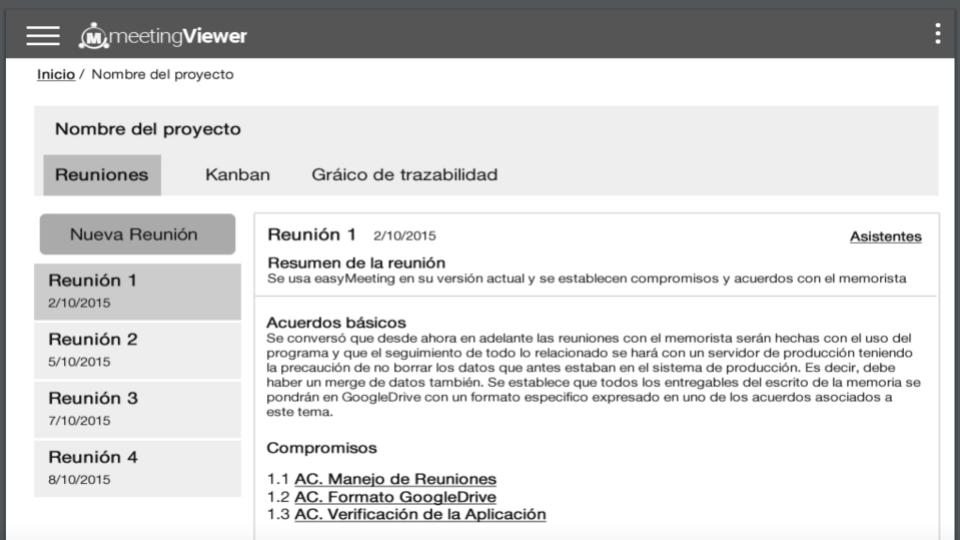
\includegraphics[width=12cm]{/versioninicial}
\caption{Bosquejo nuevo Diseño D-Minute; elaboración propia} 
\label{img4-6}
\end{figure}

Tomando de base el \textit{mockup} de la aplicación, se comenzó a desarrollar la cáscara del producto, partiendo por la imagen siguiente que corresponde al \textit{login} de la aplicación futura, ver imagen \ref{img4-7}.

\begin{figure}[!h]
\centering
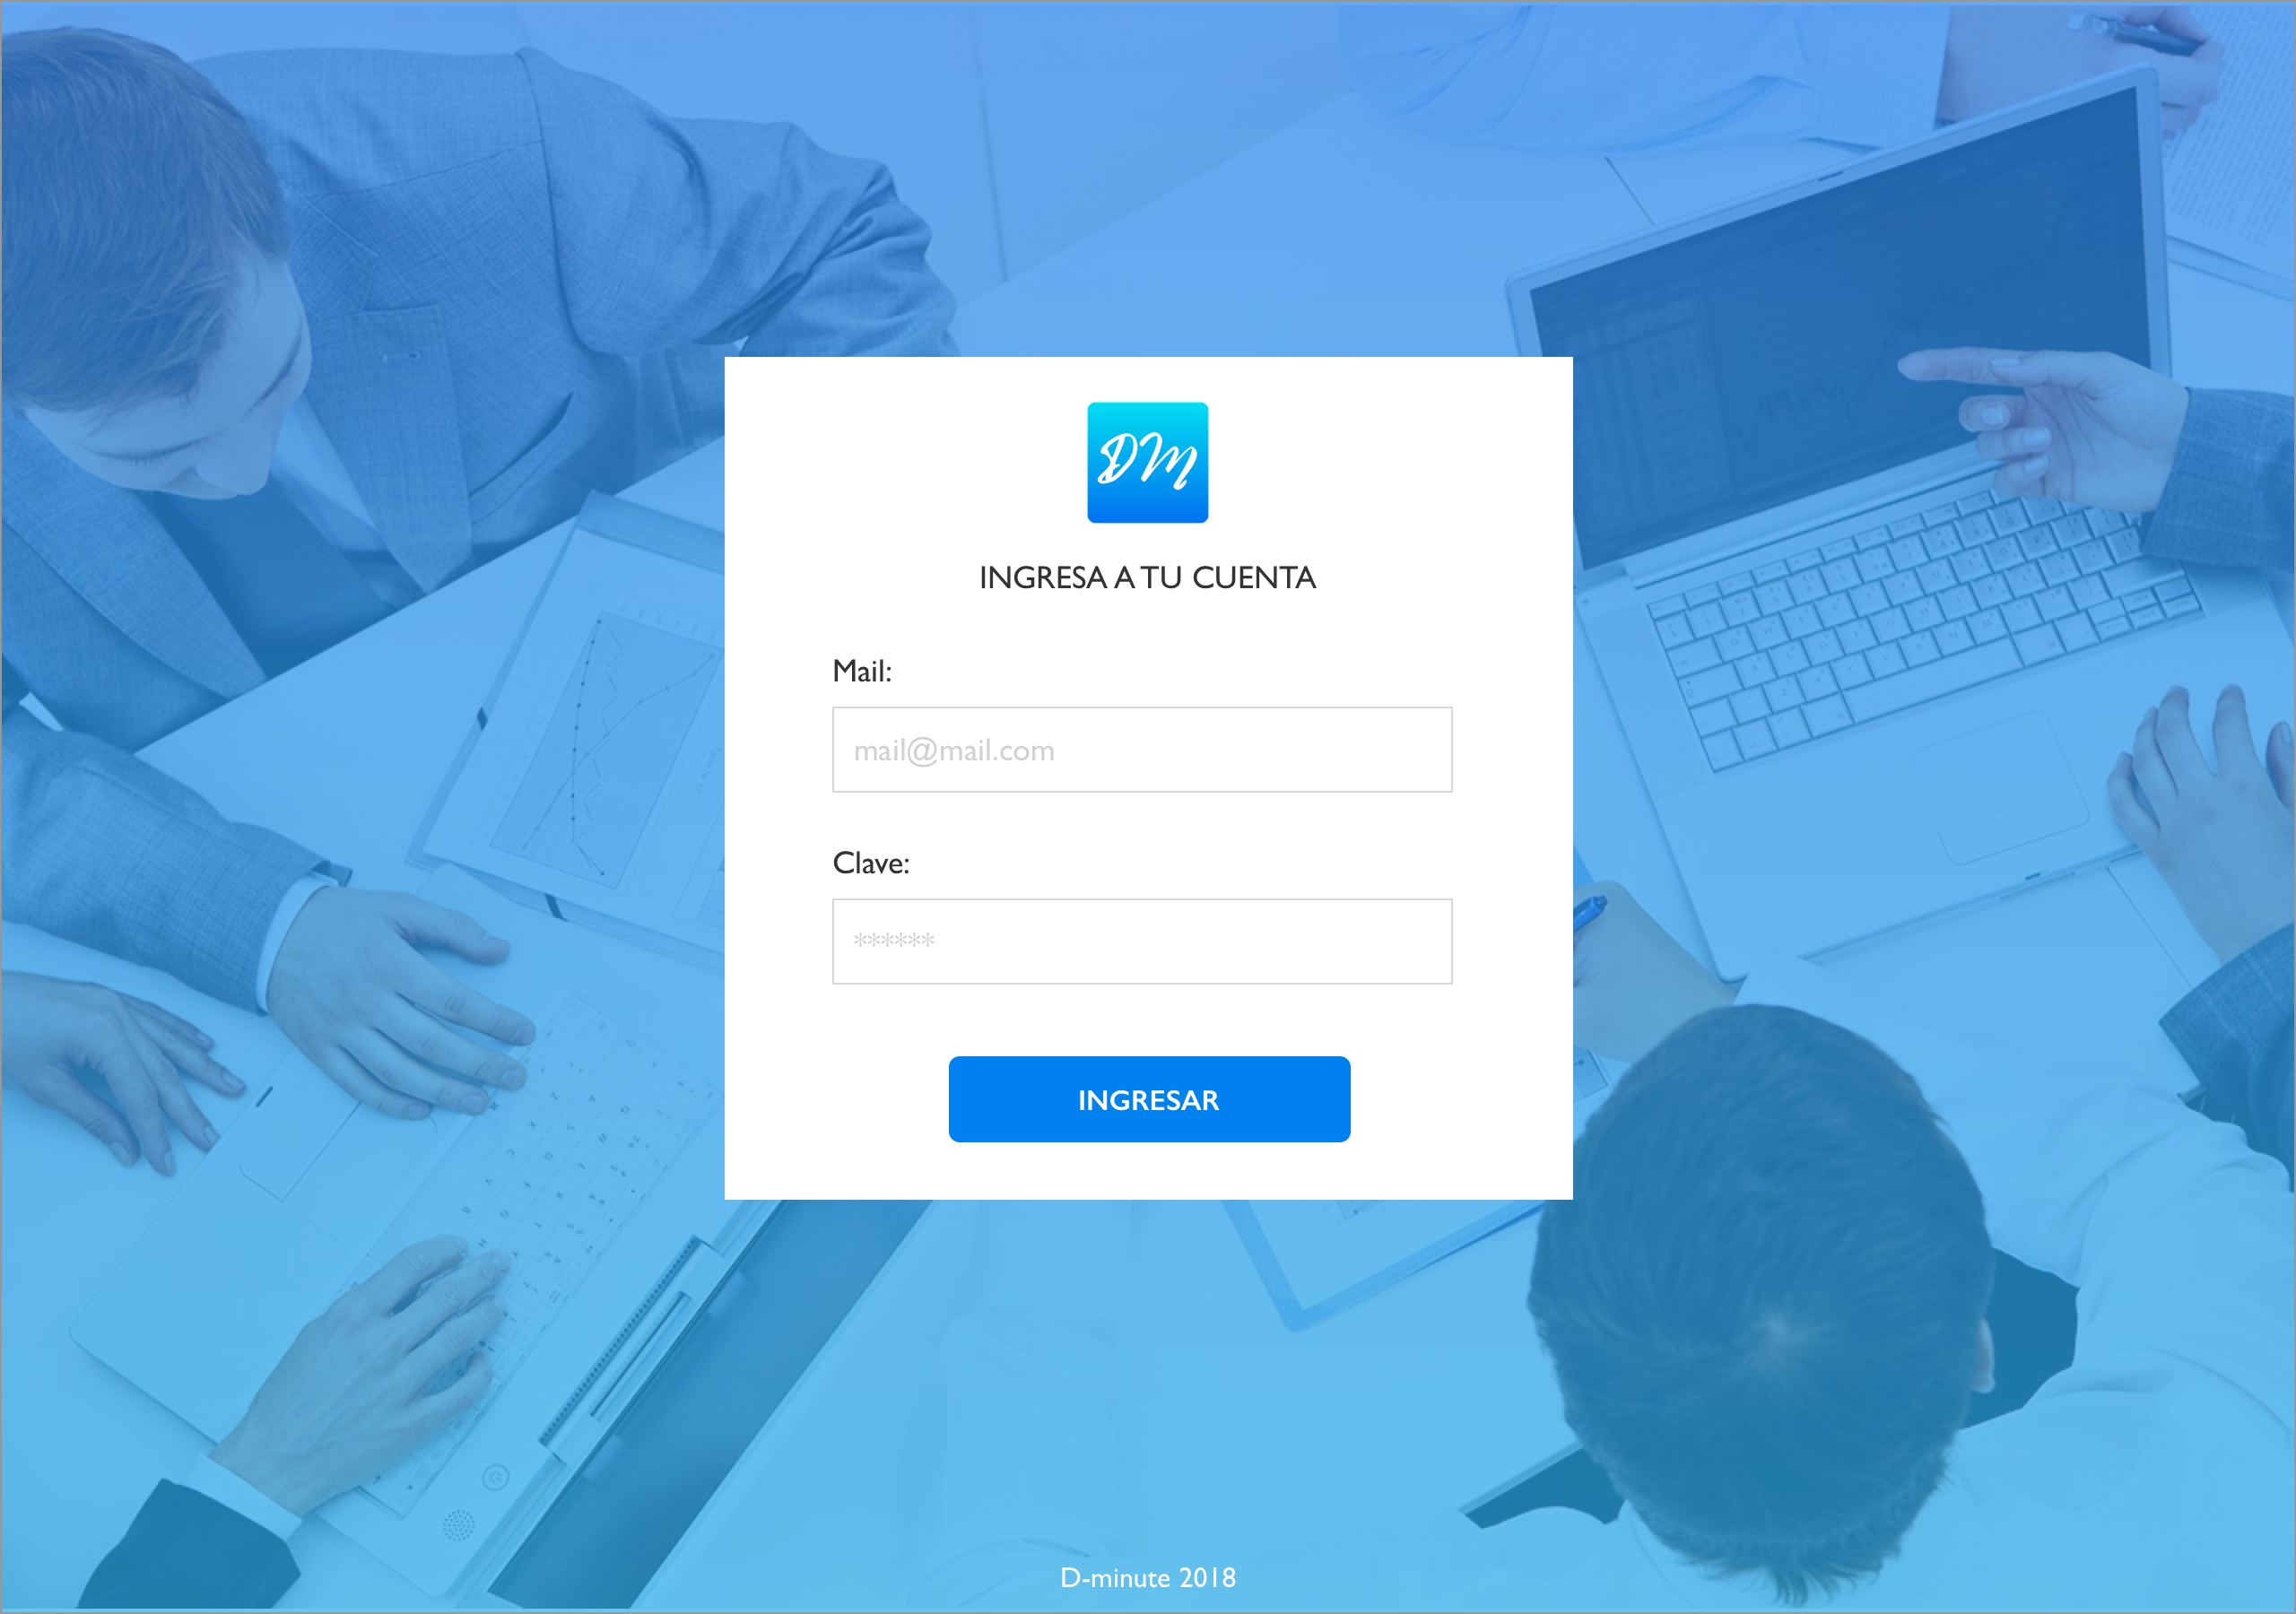
\includegraphics[width=11cm]{/app/Login_DMinute}
\caption{Diseño UX login D-Minute; elaboración propia} 
\label{img4-7}
\end{figure}

Una vez confeccionado el login fue posible establecer cuál sería el estilo de la aplicación y sus componentes asociados a utilizar, es por esto que la siguiente imagen presenta cómo se vería la opción agregar proyecto, ver imagen \ref{img4-8}.

\begin{figure}[!h]
\centering
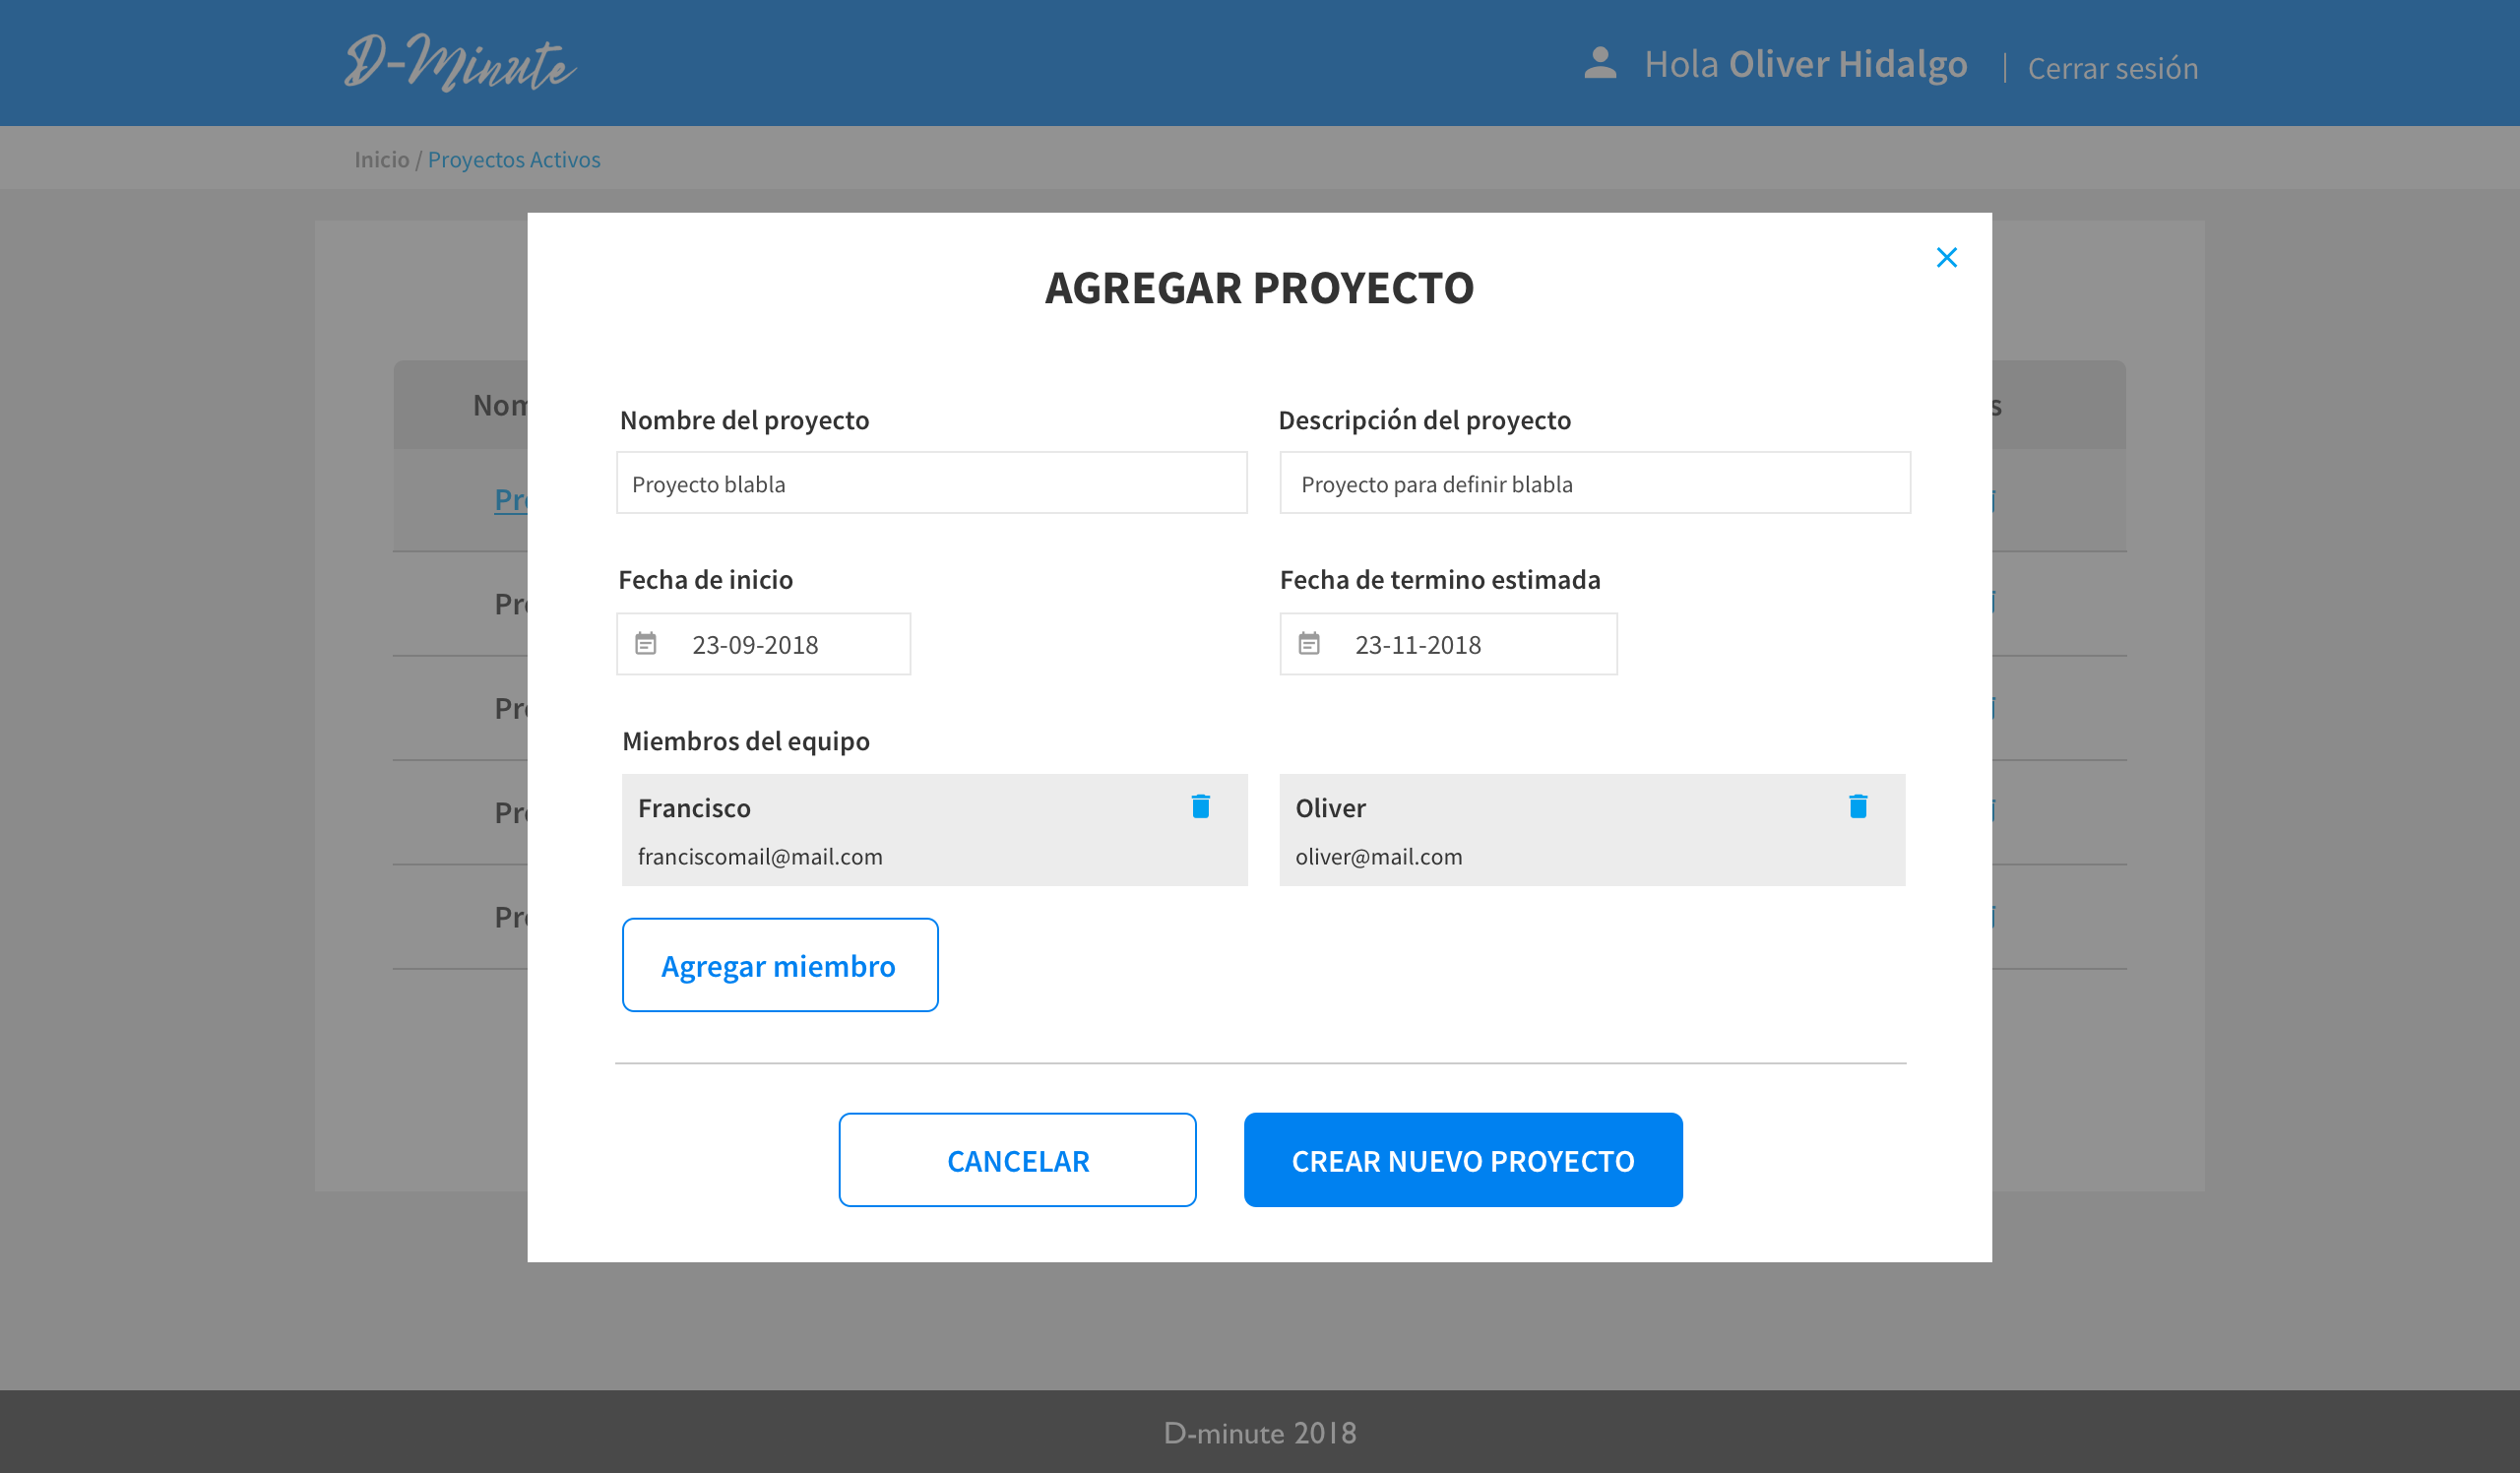
\includegraphics[width=11cm]{/app/Modal_agregarproyecto}
\caption{Diseño UX crear proyecto D-Minute; elaboración propia} 
\label{img4-8}
\end{figure}

Lo siguiente imagen corresponde al listar proyectos activos, dado que lo importante es testear el producto y no desarrollar el 100\% de funcionalidades. Lo que agrega más valor es sólo ver los proyectos activos, ver imagen \ref{img4-9}.

\begin{figure}[!h]
\centering
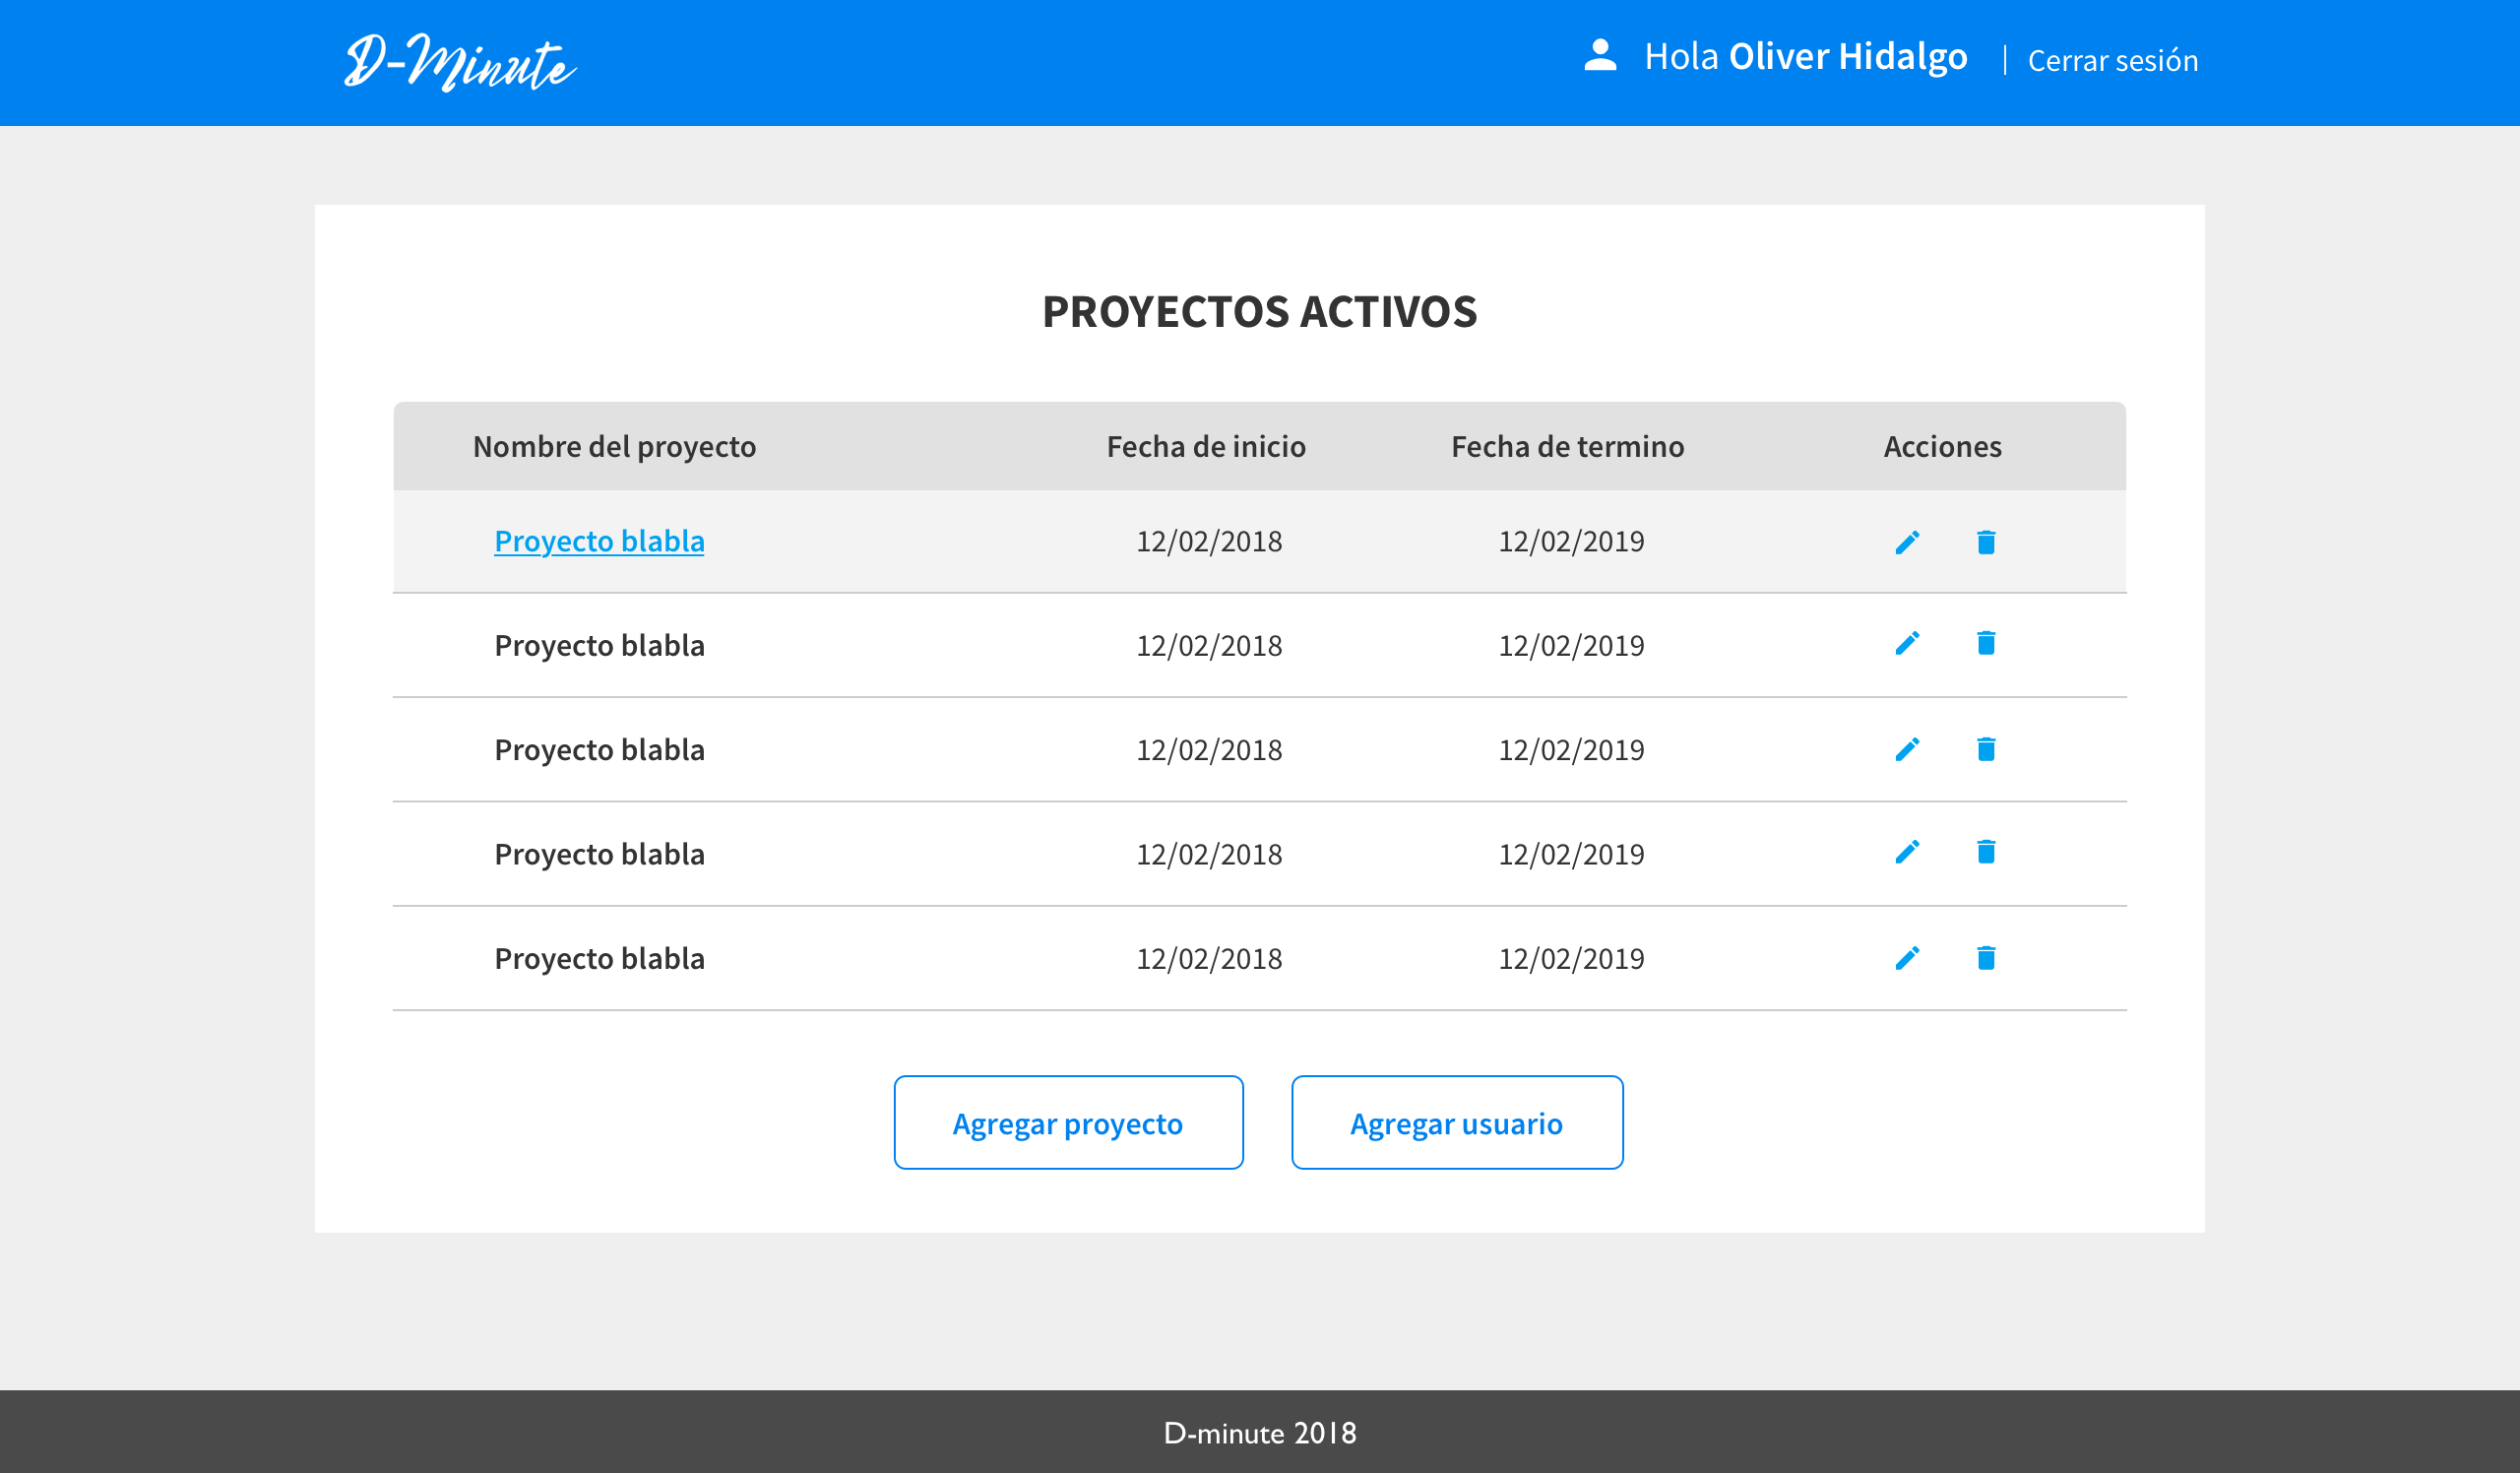
\includegraphics[width=11cm]{/app/Proyectos_Activos}
\caption{Diseño UX listar proyectos D-Minute; elaboración propia} 
\label{img4-9}
\end{figure}

Siguiendo la misma línea de dise\~no, la imagen que sigue representa cómo se vería la opción agregar reunión o acta a un proyecto activo, ver imagen \ref{img4-10}.

\begin{figure}[!h]
\centering
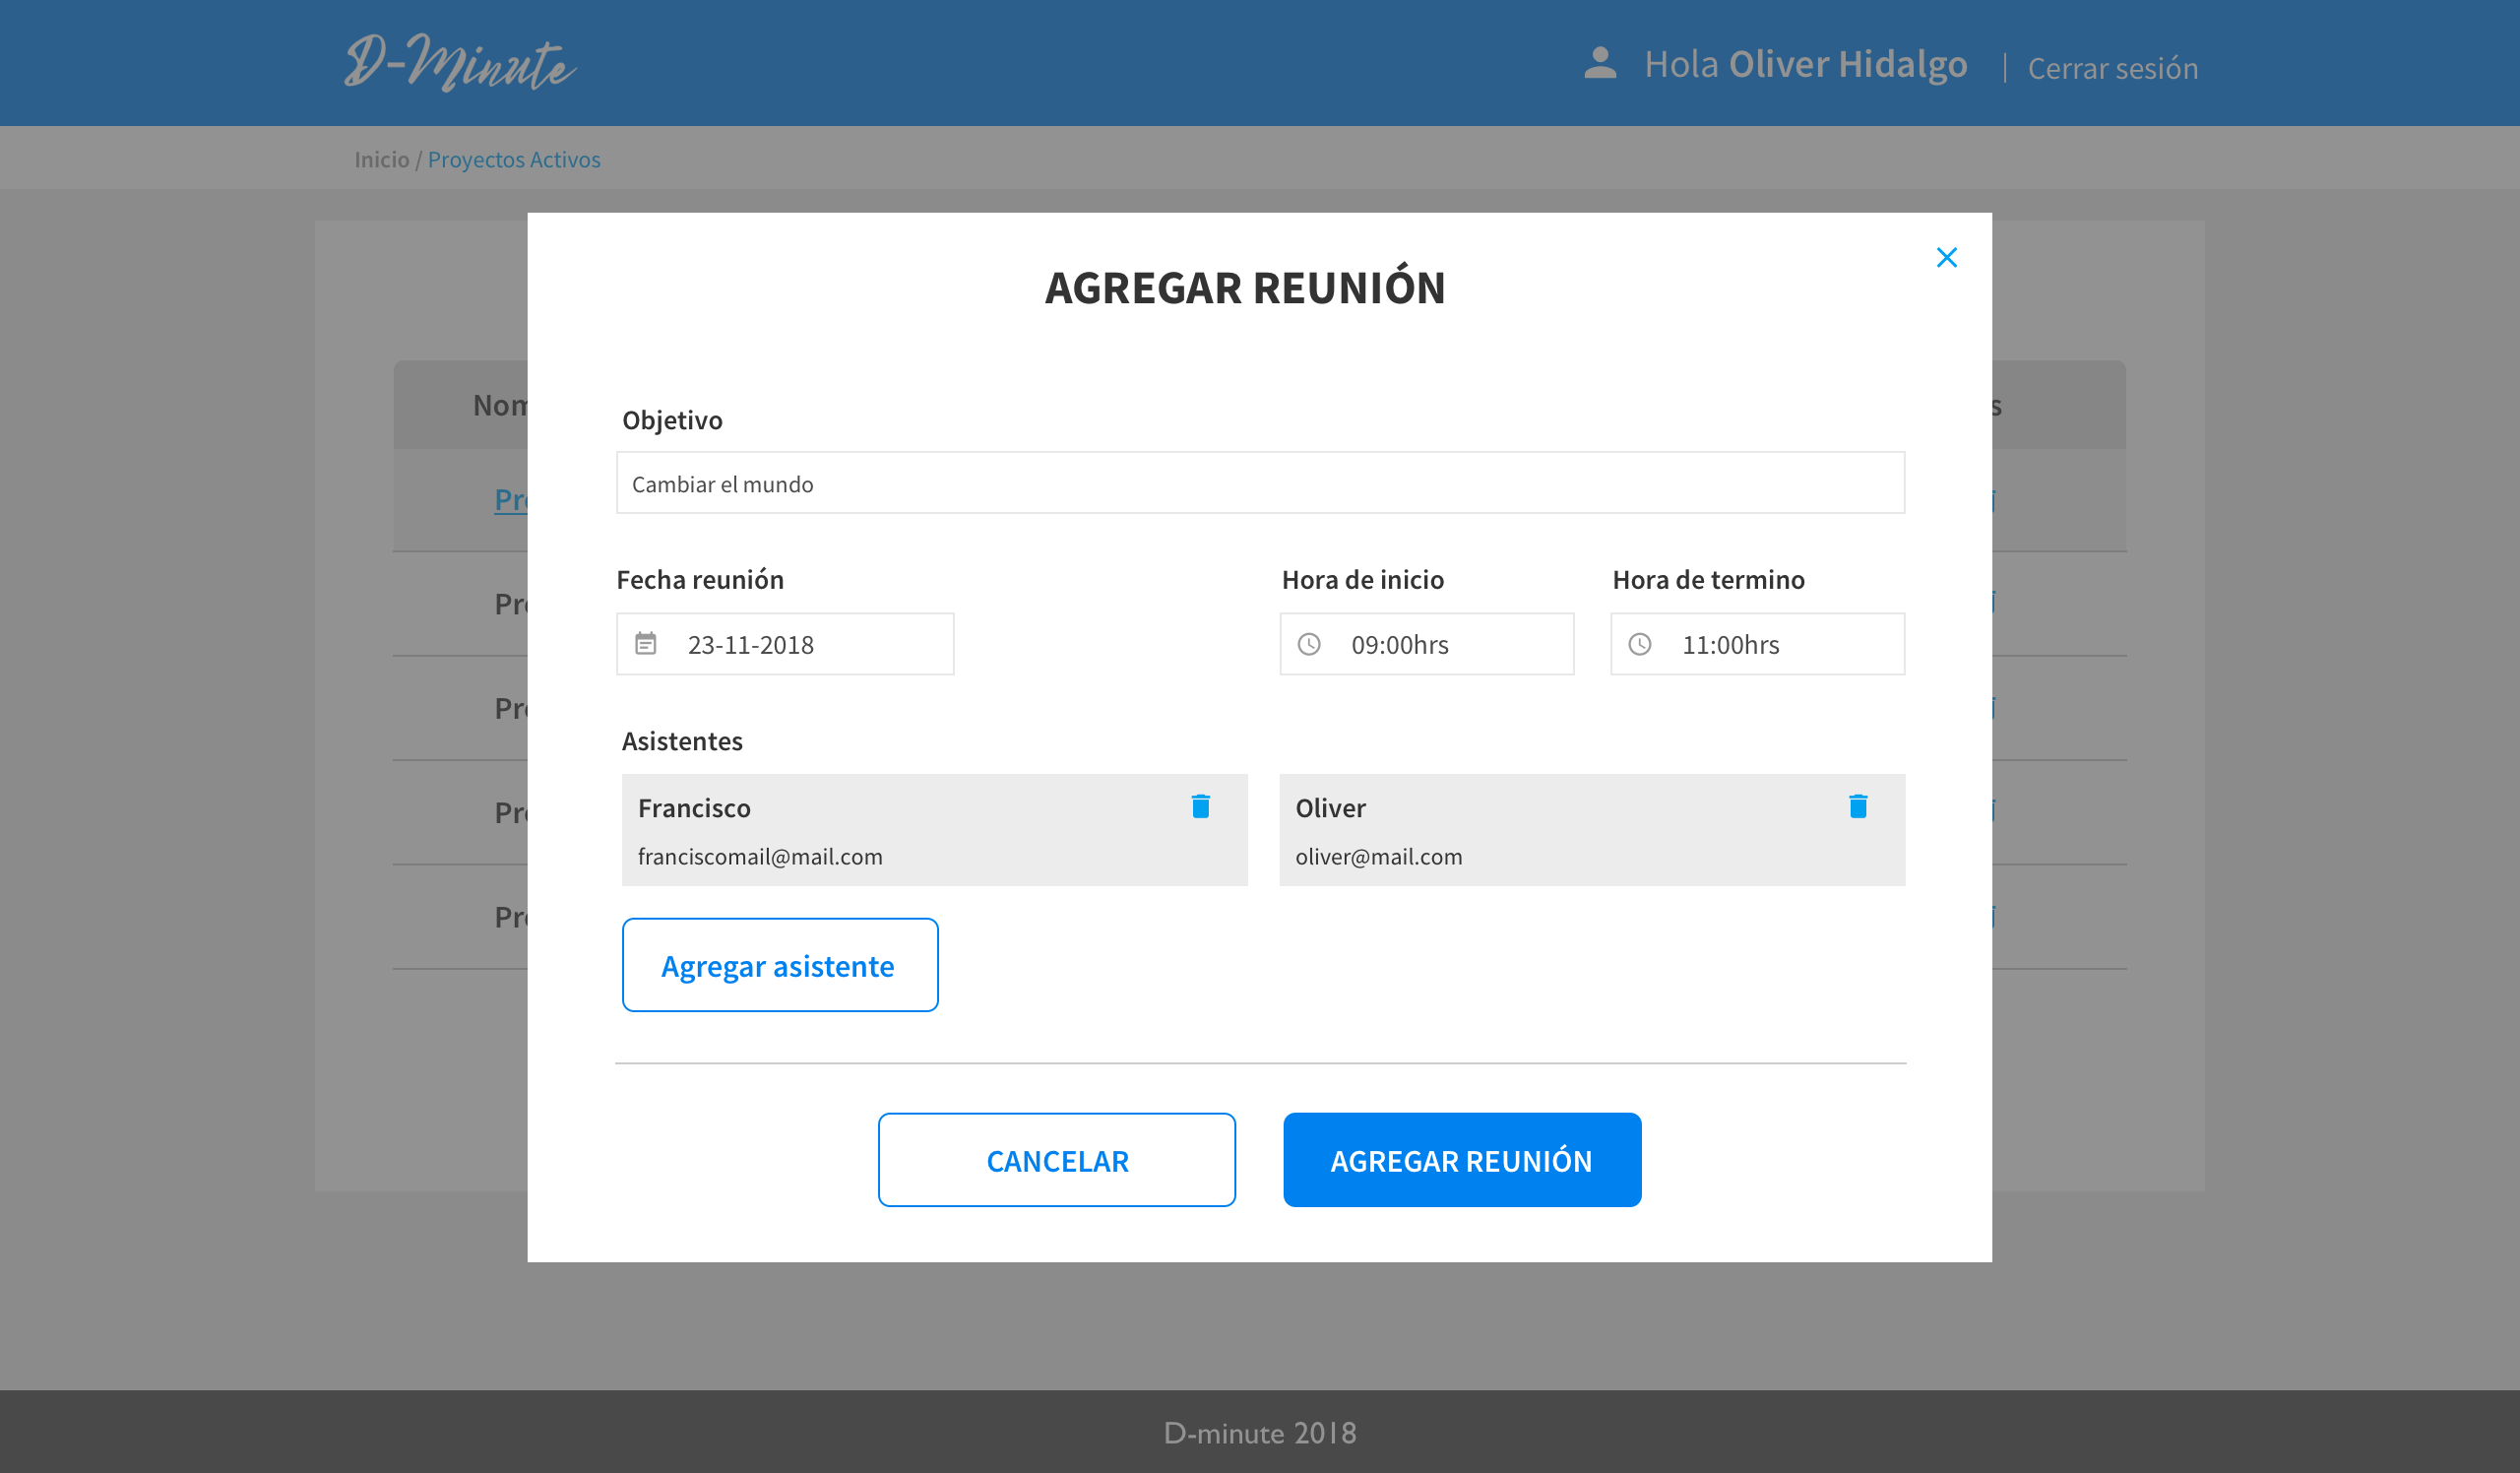
\includegraphics[width=11cm]{/app/Modal_Agregarreu}
\caption{Diseño UX crear acta D-Minute; elaboración propia} 
\label{img4-10}
\end{figure}

La siguiente imagen representa el mockup inicial, luego de haber definido la línea gráfica que tendrá la aplicación, dicha imagen expone las reuniones o actas que se desarrollan en el transcurso de un proyecto, sus temas y acciones asociadas, ver imagen \ref{img4-11}.

\begin{figure}[!h]
\centering
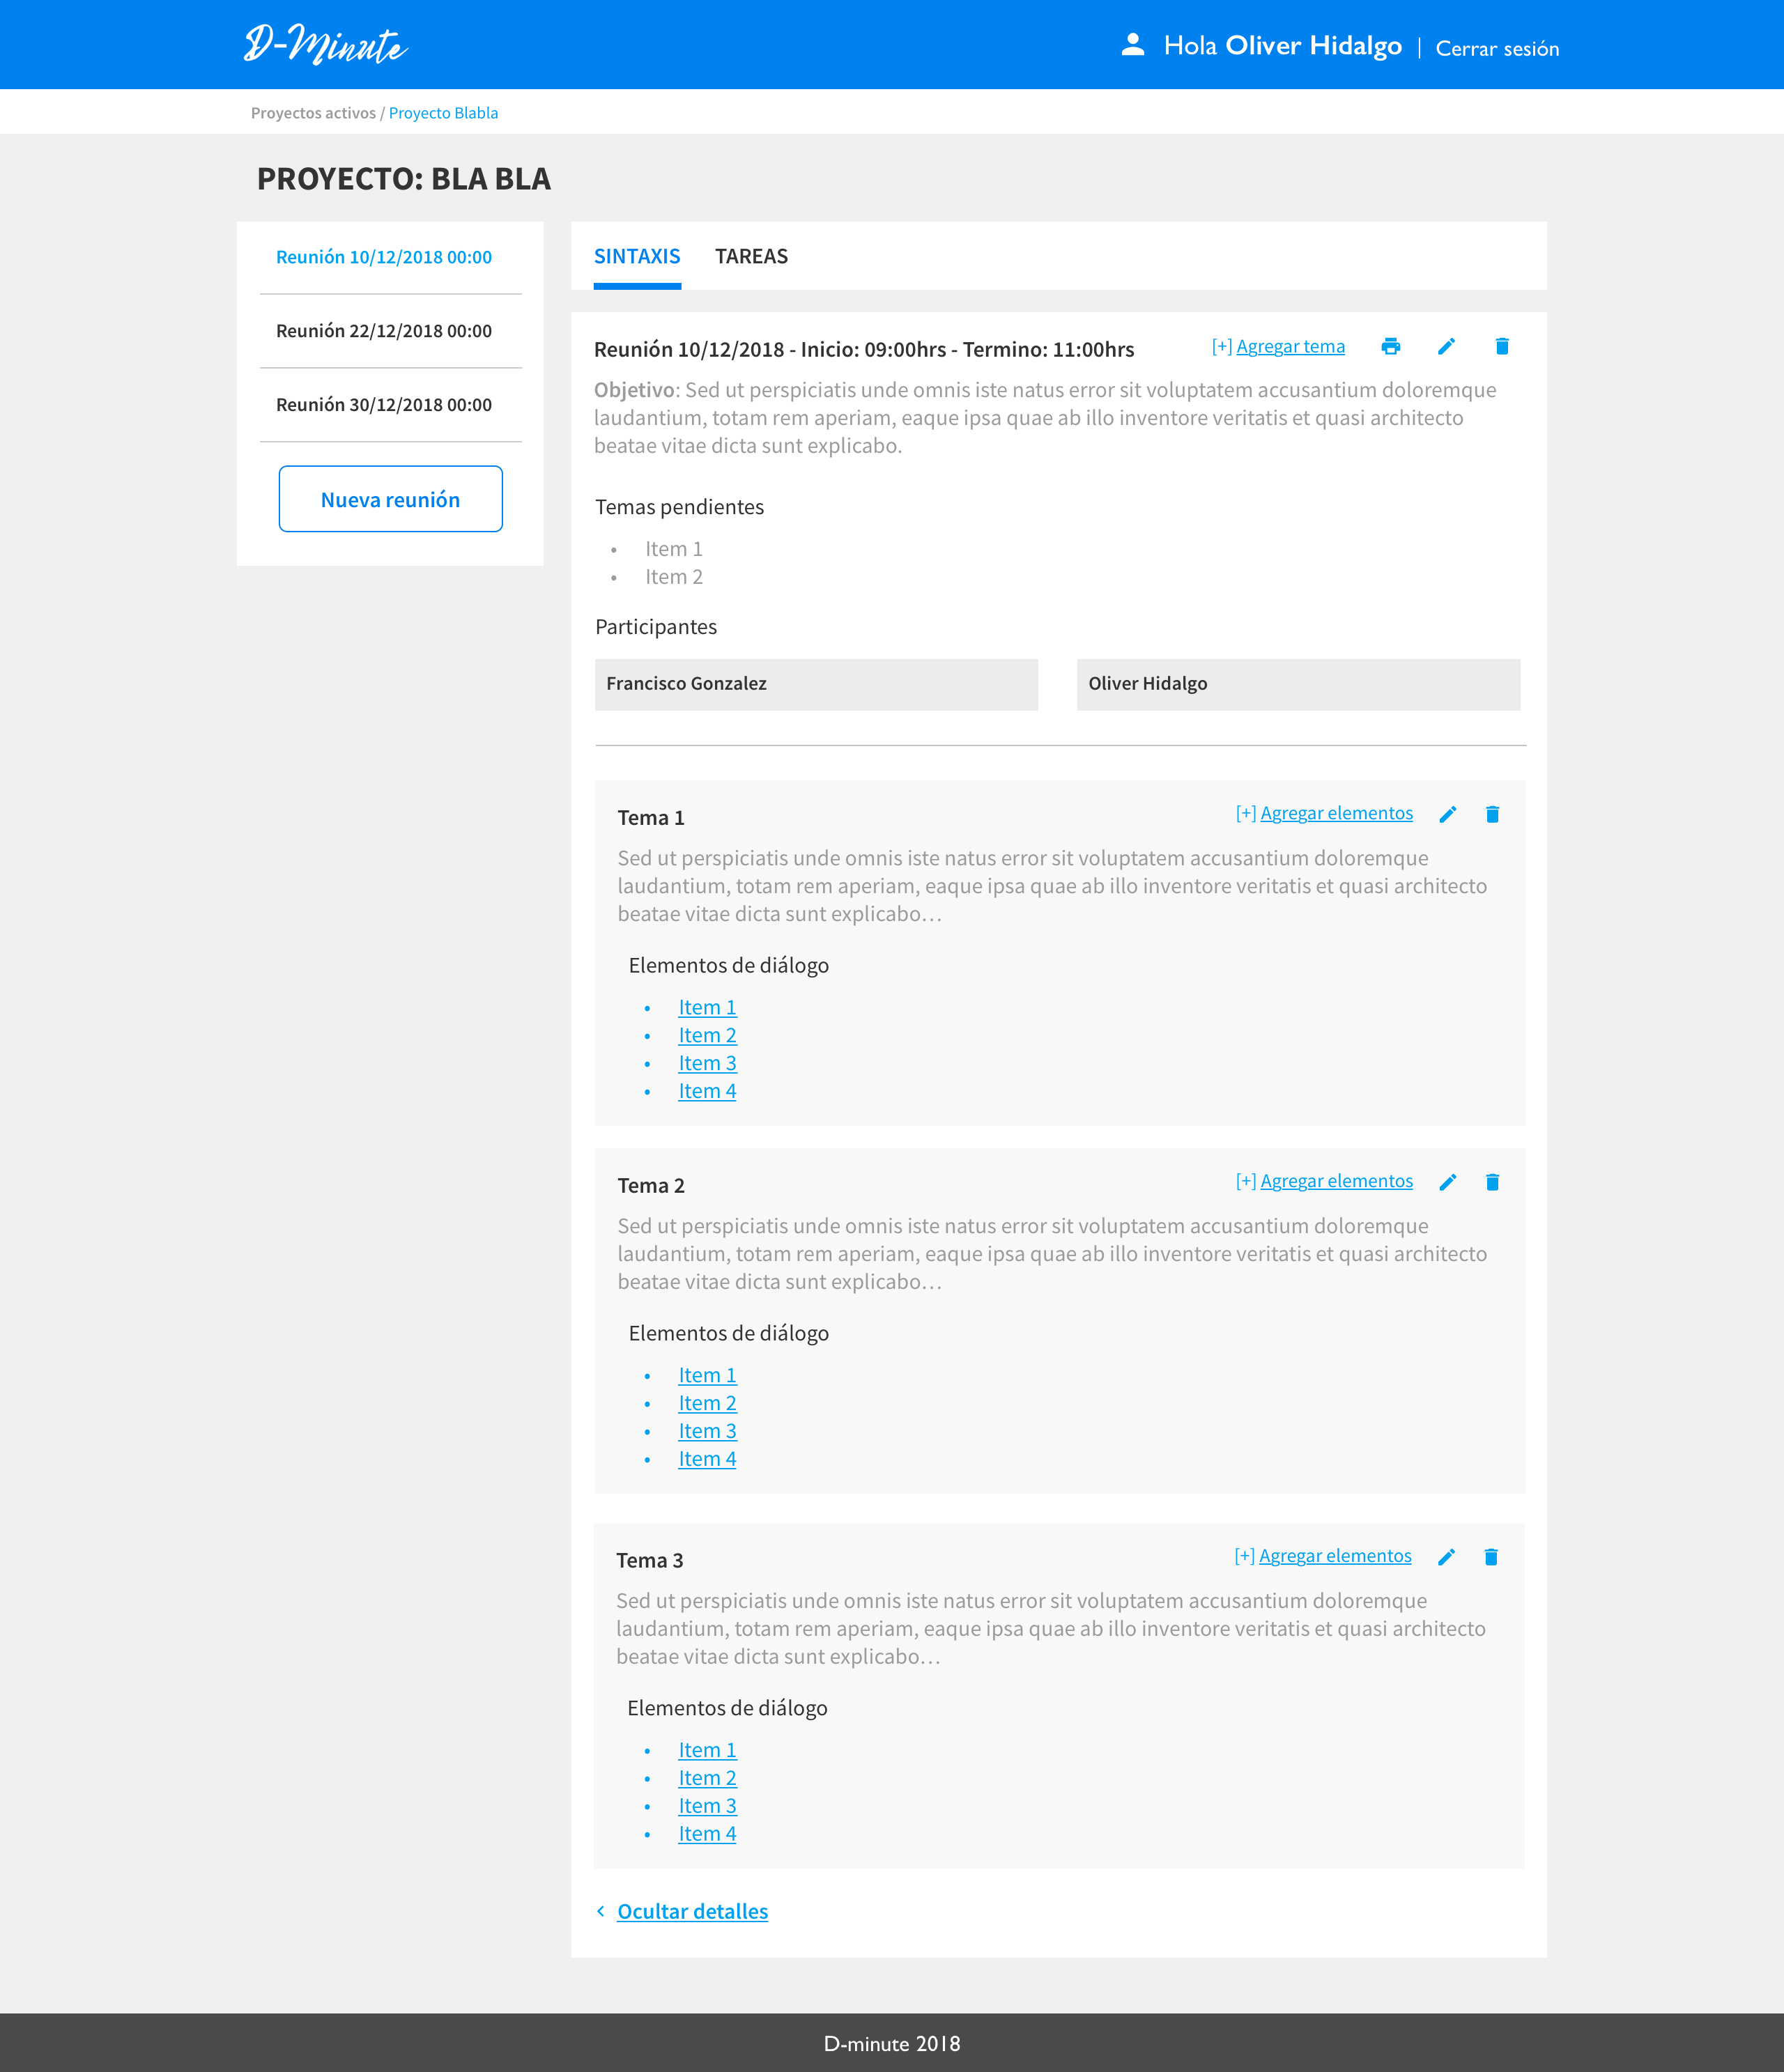
\includegraphics[width=13cm]{/app/despliegue}
\caption{Diseño UX reuniones de trabajo D-Minute; elaboración propia} 
\label{img4-11}
\end{figure}

Uno de los puntos más relevantes representados en la siguiente imagen, tiene relación con agregar los elementos de diálogos - duda, acuerdo, compromiso, desacuerdo y norma - a un tema que es parte de una reunión de trabajo, ver imagen \ref{img4-12}.

\begin{figure}[!h]
\centering
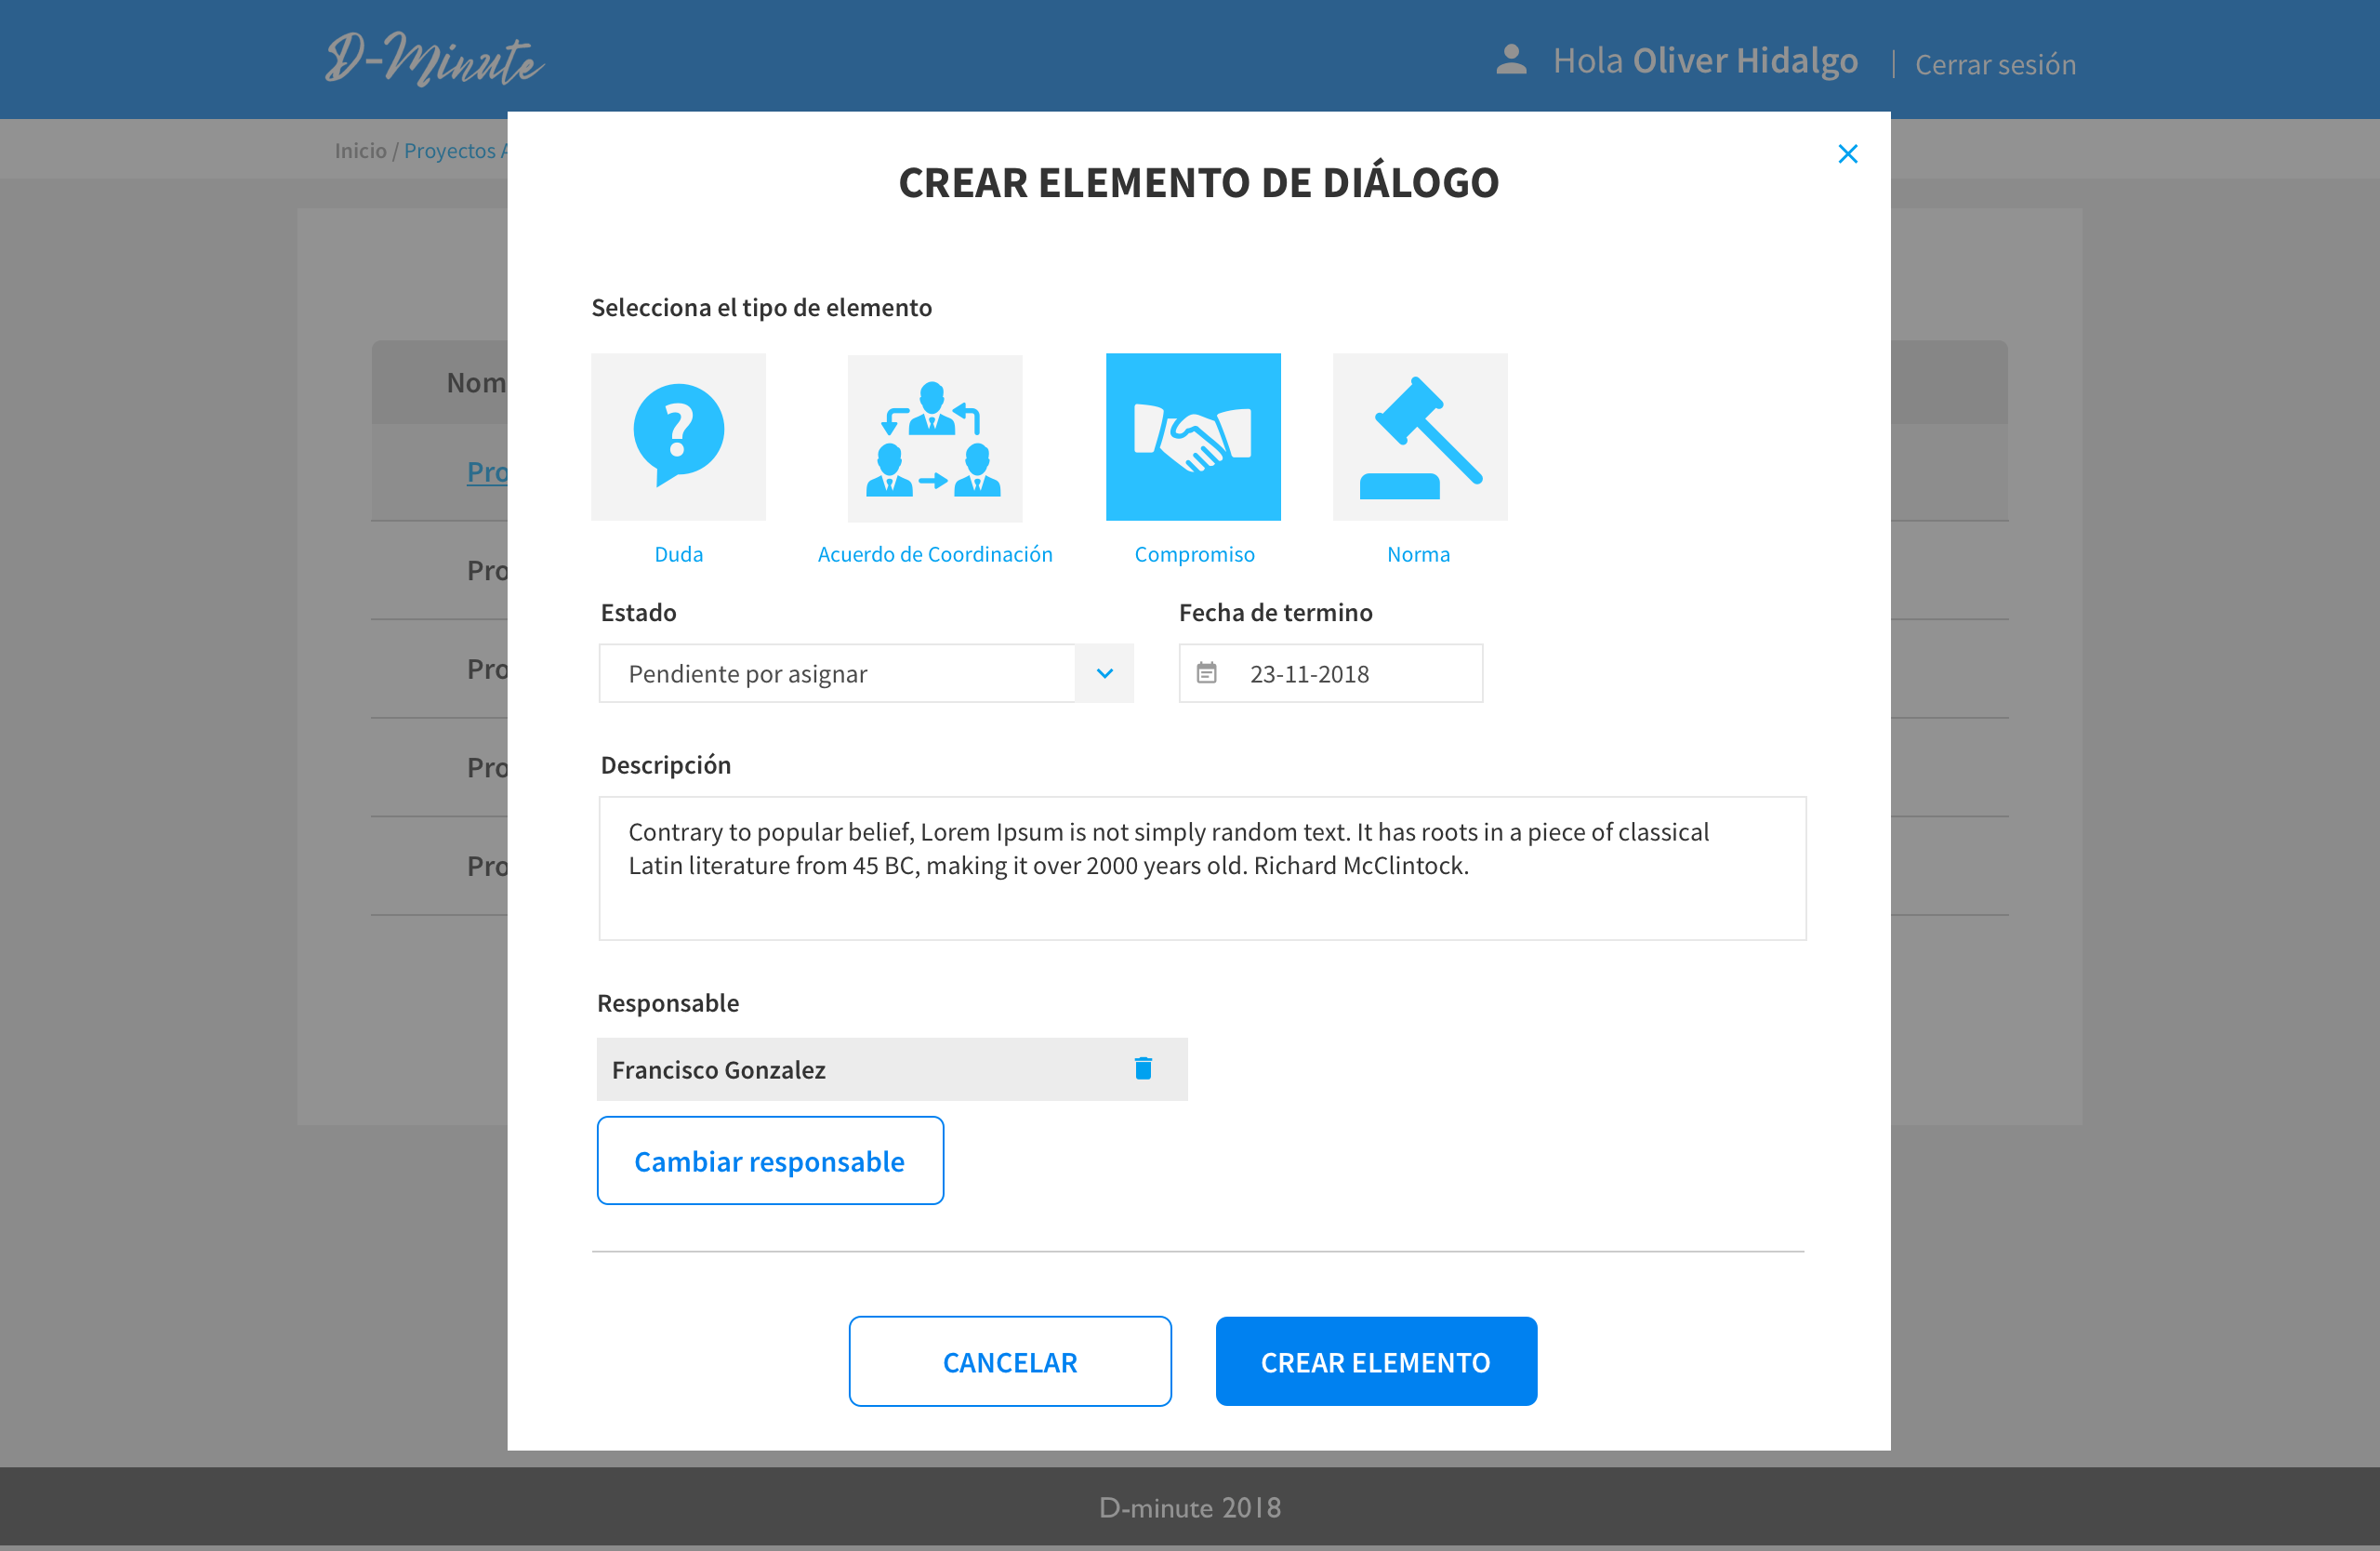
\includegraphics[width=11cm]{/app/Modal_Elemento_select_}
\caption{Diseño UX agregar elemento de diálogo D-Minute; elaboración propia} 
\label{img4-12}
\end{figure}

Por último con el fin de dar trazabilidad a los elementos, la siguiente imagen representa las acciones que tiene un proyecto en un tablero de tareas, ver imagen \ref{img4-13}.

\begin{figure}[!h]
\centering
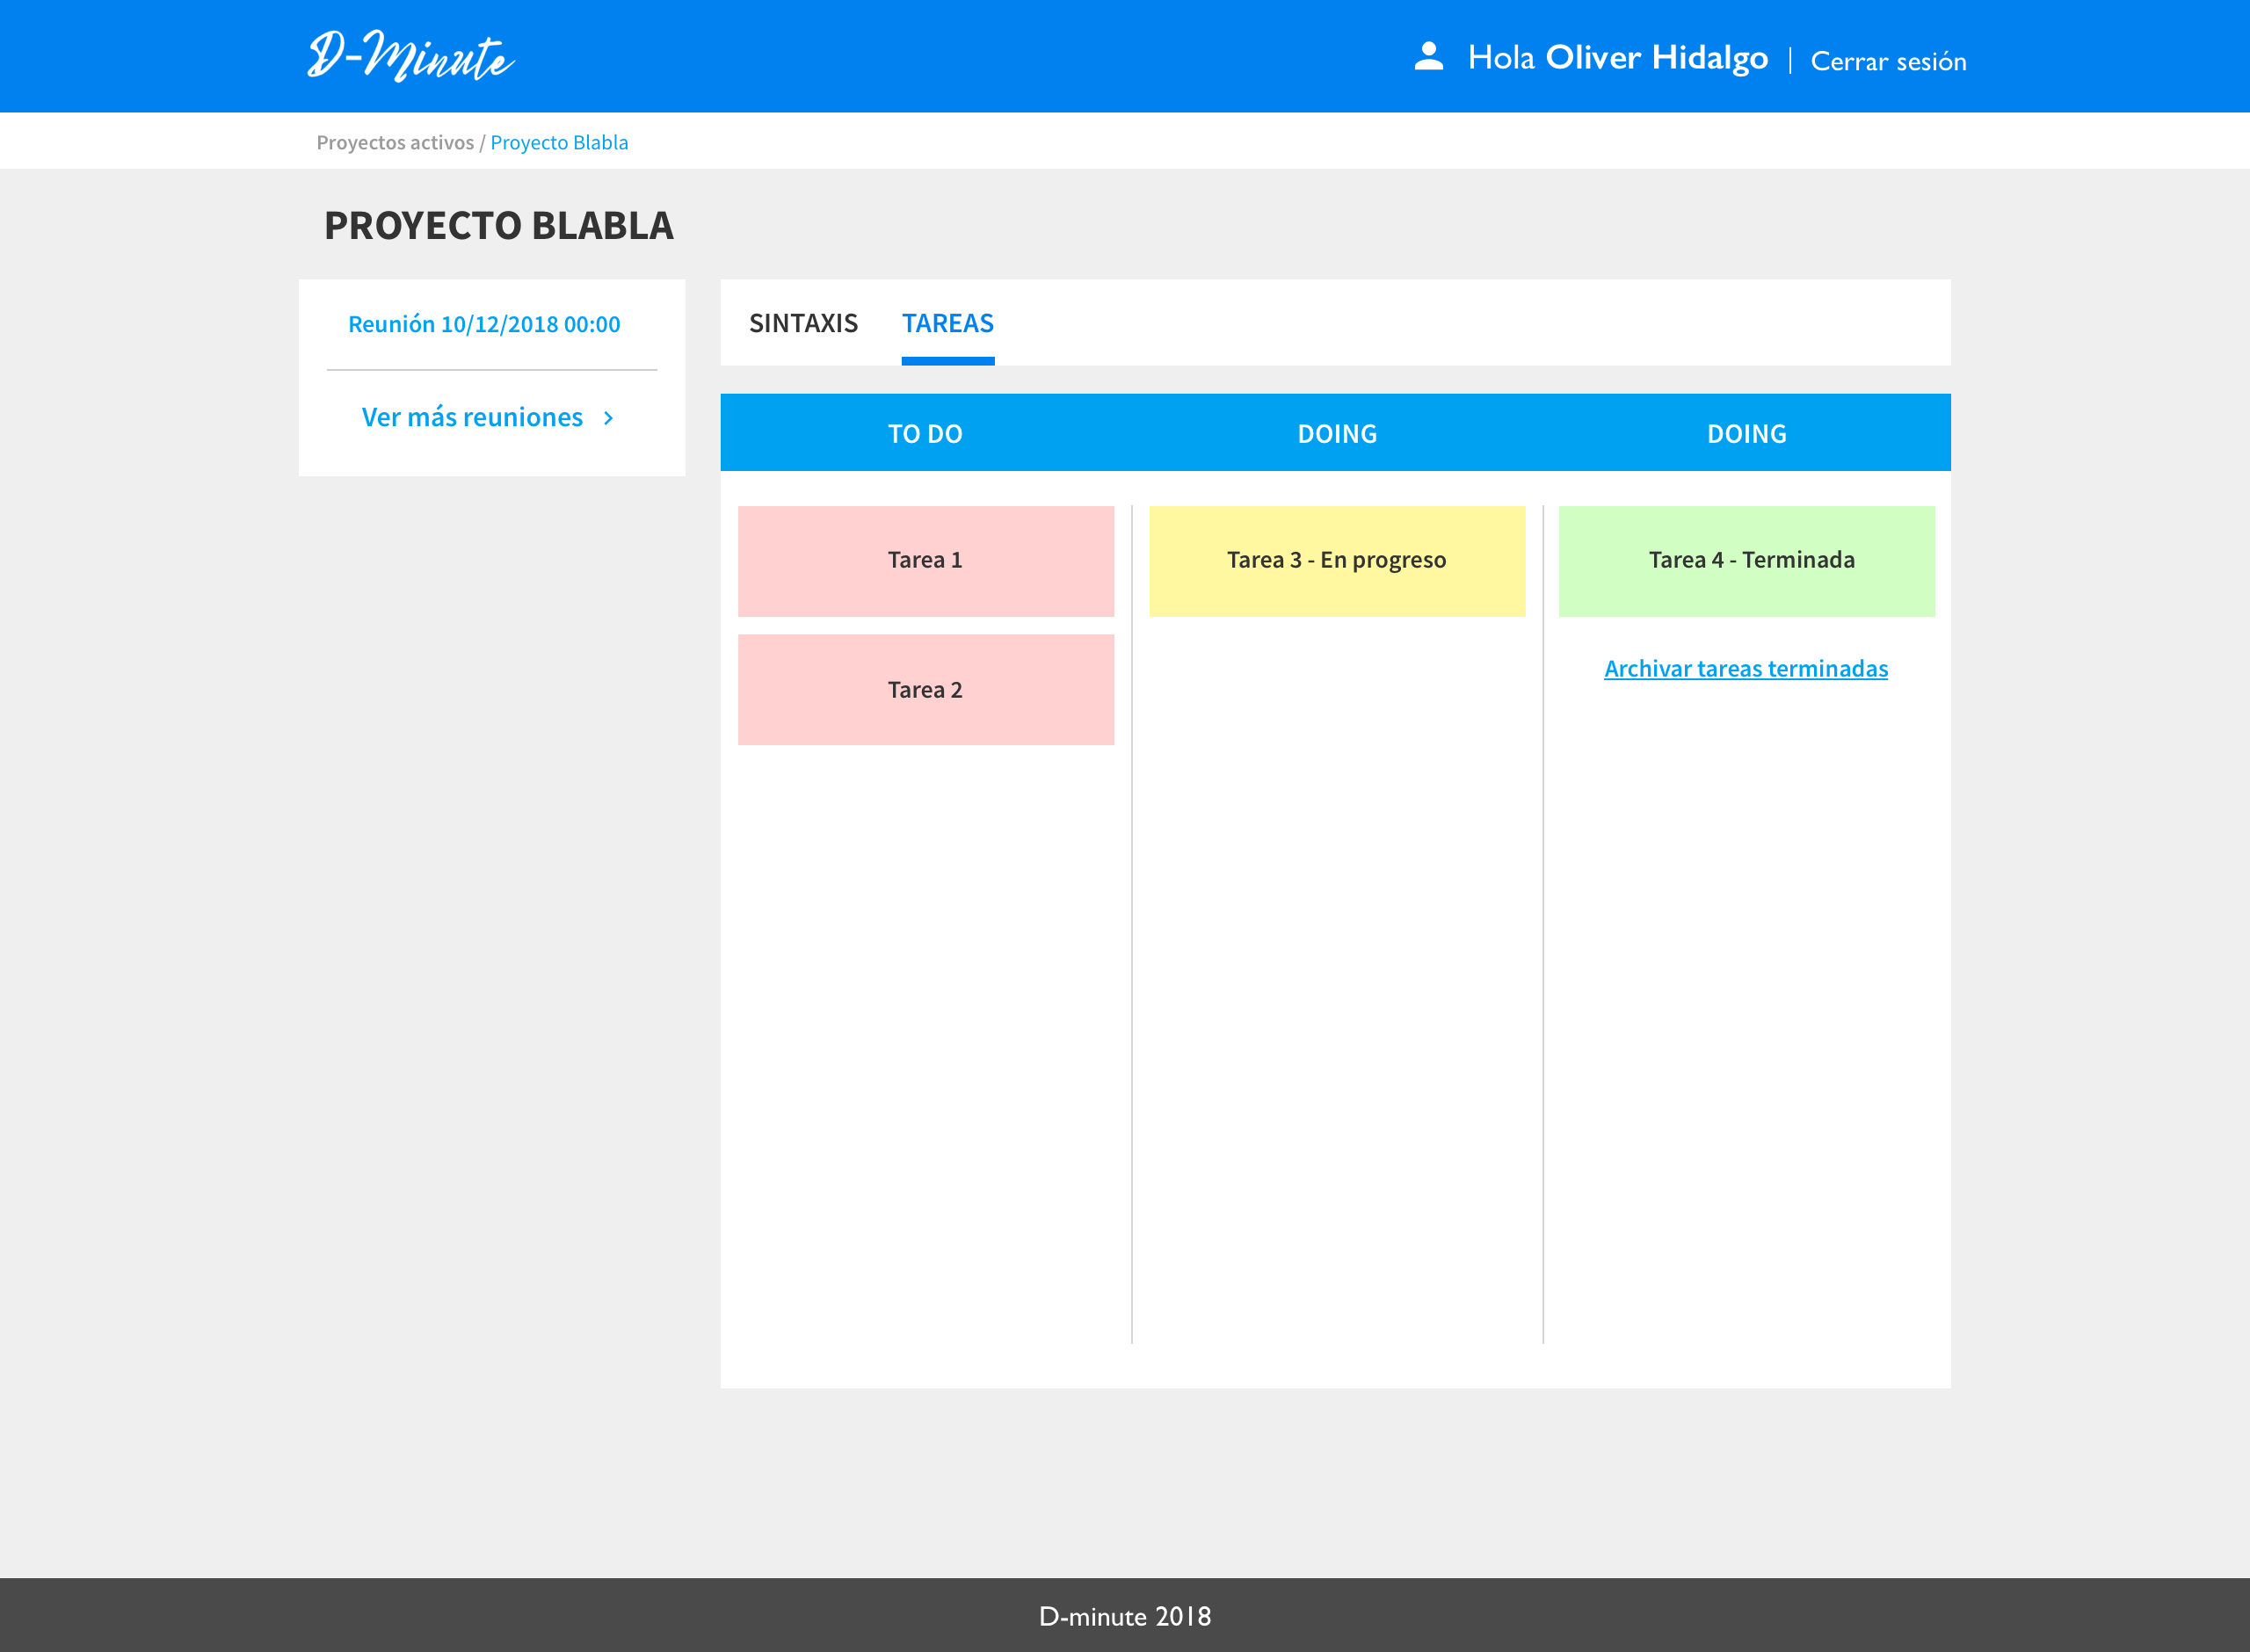
\includegraphics[width=11cm]{/app/tareas}
\caption{Diseño UX Kanban de tareas D-Minute; elaboración propia} 
\label{img4-13}
\end{figure}

\subsection{ARQUITECTURA}

\subsubsection{\textit{Front-End}}

Para el desarrollo de la parte \textit{front-end} se acuerda trabajar con \textbf{Angular 5} dado sus ventajas\footnote{Ver ventajas en: \url{https://www.campusmvp.es/recursos/post/angular-5-todo-lo-que-necesitas-saber-en-10-minutos-o-menos.aspx}} sobre otros lenguajes de programación y la velocidad que se puede dar al desarrollo trabajando con \textit{mockups} para no depender del \textit{back-end}. Lo anterior, sumado a la expertise del equipo.

\subsubsection{\textit{Back-End}}

Para el desarrollo de la parte \textit{back-end} se acuerda trabajar microservicios en \textbf{Spring Boot} con java 1.8 utilizando maven como repositorio de librerías \textit{Release}. \textit{Spring} es uno de los framework que más esta siendo utilizados\footnote{Ver beneficios en : \url{https://es.linkedin.com/pulse/porque-me-gusta-trabajar-con-arquitectura-de-spring-boot-danilo-rodas
}} hoy en día por la gran cantidad de beneficios que ofrece, documentación y dinamismo al momento de generar el desarrollo.

\subsubsection{Base Datos}

Como gestor de datos se acuerda trabajar con MySQL en su versión 5.0 debido a que es una base datos \textit{opensource} con un excelente rendimiento y se acopla bastante bien con aplicación en la nube. 
El modelo no puede ser presentado debido a que a medida que se va construyendo el \textit{software} se va definiendo lo que se necesita con el fin de no gastar tiempo en cosas que no aportan valor.

\subsubsection{\textit{Platform as a Service (Paas)}}

Dado que el desarrollo de D-Minute será llevado a cabo en micro arquitectura, se acuerda utilizar Heroku\footnote{Heroku: \url{https://es.wikipedia.org/wiki/Heroku}} como Paas en la nube. Debido a que su servicio gratuito ofrece muchas ventajas para el despliegue y seguimiento de la aplicación como también un soporte para alta disponibilidad, ver imagen plataforma \ref{img4-14}.

\begin{figure}[!h]
\centering
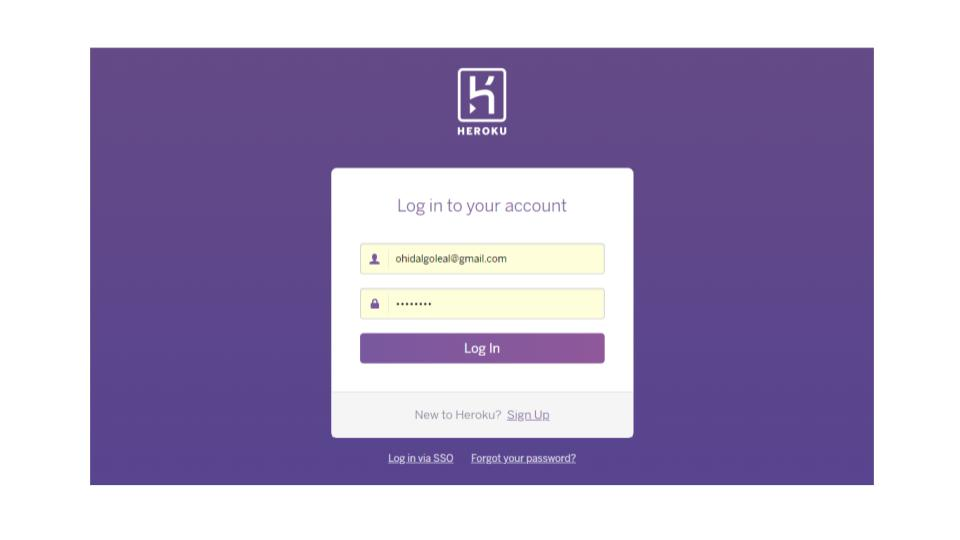
\includegraphics[width=11cm]{/heroku}
\caption{PaaS Heroku; tomado de Heroku} 
\label{img4-14}
\end{figure}

\subsubsection{Diagrama de Arquitectura}

El siguiente diagrama de arquitectura fue acordado con el equipo para dar a conocer la forma que será abordado el desarrollo y tener una visión general de cómo estará construido el producto, ver imagen \ref{img4-15}.

\begin{figure}[!h]
\centering
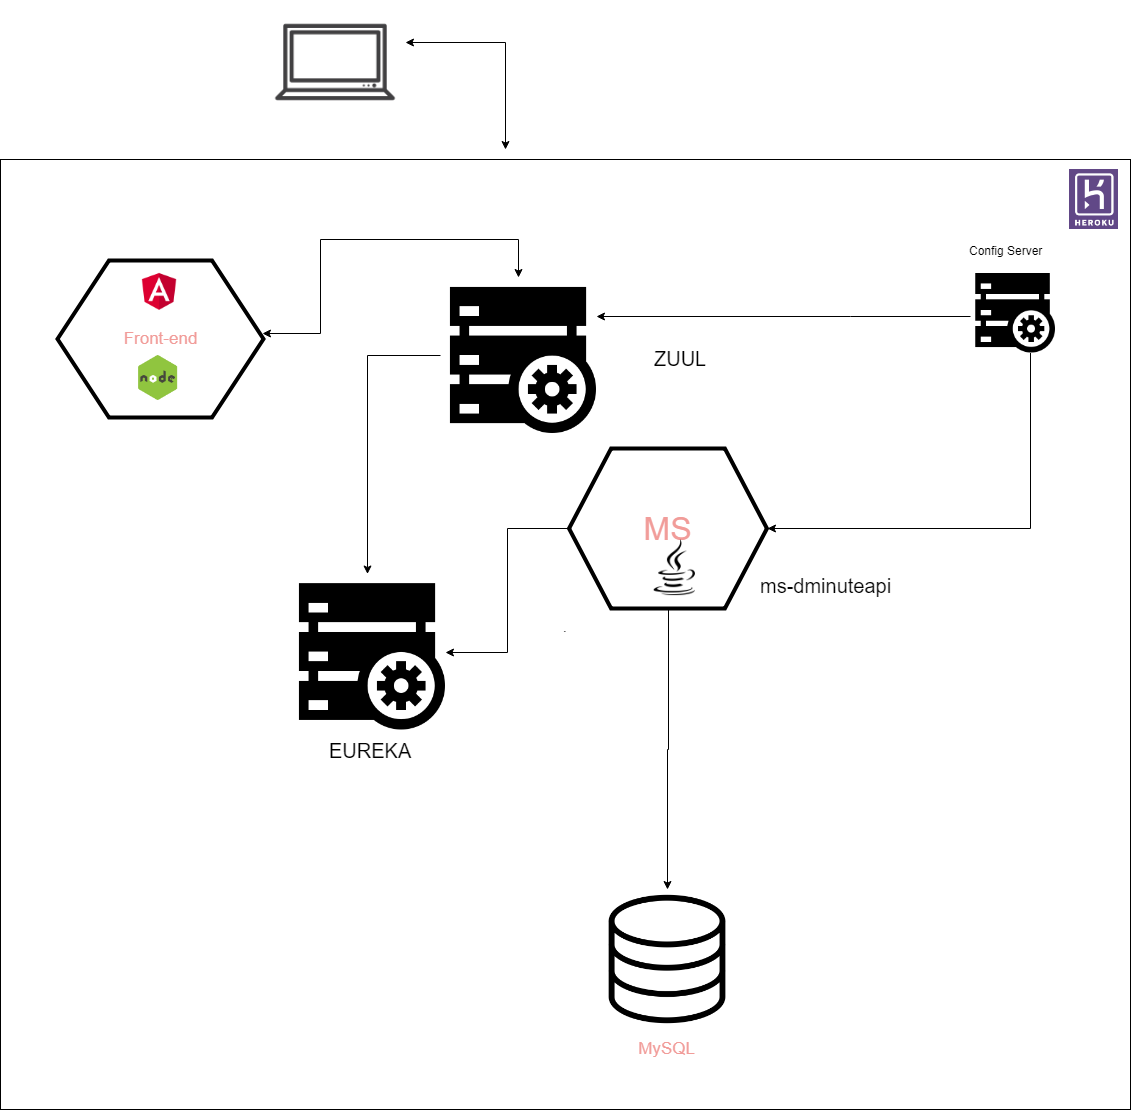
\includegraphics[width=11cm]{/disenioArquitectura}
\caption{Dise\~no Arquitectura D-Minute; elaboración propia} 
\label{img4-15}
\end{figure}

\subsection{DESARROLLO PRODUCTO EN \textit{SPRINT}}

A continuación se detalle el desarrollo del producto en \textit{sprint} y las historias de usuario comprometidas:

\begin{itemize}
	\item \textbf{\textit{Sprint} 1:} Configurar ambientes para desarrollo. Ver \textit{spring backlog} en tabla \ref{tab:backlog1}

\begin{table}[!h]
\centering
\caption{\textit{Sprint} uno, \textit{Sprint Backlog}: Preparar ambiente \textit{Developer}, Refactorización temas acta, elaboración propia}
\label{tab:backlog1}
\begin{tabular}{|l|l|r|}
\hline
\multicolumn{1}{|c|}{\textit{\textbf{Feature}}} & \textbf{Epica} & \textbf{Peso} \\ \hline
Configuración ambiente DMinute & Técnica & 3 \\ \hline
Levantar aplicación web en Heroku & Técnica & 3 \\ \hline
Refactorización de código para creación de temas de la reunión & Técnica & 8 \\ \hline
\end{tabular}
\end{table}

	\item \textbf{\textit{Sprint} 2:} Desarrollar APIs de servicios para la creación de actas y elementos de diálogo. Ver \textit{spring backlog} en tabla \ref{tab:backlog2}

\begin{table}[!h]
\centering
\caption{\textit{Sprint} dos, \textit{Sprint Backlog}: Refactorización acta y elementos de diálogo, elaboración propia}
\label{tab:backlog2}
\begin{tabular}{|l|l|r|}
\hline
\multicolumn{1}{|c|}{\textit{\textbf{Feature}}} & \textbf{Epica} & \textbf{Peso} \\ \hline
Refactorización de código para creación elementos de diálogo & Técnica & 8 \\ \hline
Refactorización de código para creación de minutas & Técnica & 8 \\ \hline
\end{tabular}
\end{table}

	\item \textbf{\textit{Sprint} 3:} Generar estructura de proyecto \textit{front-end} en angular 5. Ver \textit{spring backlog} en tabla \ref{tab:backlog3}

\begin{table}[!h]
\centering
\caption{\textit{Sprint} tres, \textit{Sprint Backlog}: Refactorización acta y elementos de diálogo, elaboración propia}
\label{tab:backlog3}
\begin{tabular}{|l|l|r|}
\hline
\multicolumn{1}{|c|}{\textit{\textbf{Feature}}} & \textbf{Epica} & \textbf{Peso} \\ \hline
Implementación nueva estructura UX & Técnica & 8 \\ \hline
Eliminar envio de correo en creación usuario & Técnica & 3 \\ \hline
Cambiar librería de input de textos & Generación Acta & 3 \\ \hline
\textit{Spike} -  Revisar librería Kanban tareas & Seguimiento de tareas & 2 \\ \hline
\end{tabular}
\end{table}

	\item \textbf{\textit{Sprint} 4:} Migrar por completa aplicación de python a microarquitectura e implementar modelo final de base datos. Ver \textit{spring backlog} en tabla \ref{tab:backlog4}

\begin{table}[!h]
\centering
\caption{\textit{Sprint} cuatro, \textit{Sprint Backlog}: Reestructurar menú actas y listar acta, elaboración propia}
\label{tab:backlog4}
\begin{tabular}{|l|l|r|}
\hline
\multicolumn{1}{|c|}{\textit{\textbf{Feature}}} & \textbf{Epica} & \textbf{Peso} \\ \hline
Reestructurar Menú Creación de Actas & Evolución UX & 5 \\ \hline
Reestructurar Listado de Minutas & Evolución UX & 8 \\ \hline
\end{tabular}
\end{table}

	\item \textbf{\textit{Sprint} 5:} Implementar modelo de micro servicios en \textit{cloud} y generar estilos estándar de la aplicación. Ver \textit{spring backlog} en tabla \ref{tab:backlog5}

\begin{table}[!h]
\centering
\caption{\textit{Sprint} cinco, \textit{Sprint Backlog}: Visualizar detalle minuta y normalizar estilos, elaboración propia}
\label{tab:backlog5}
\begin{tabular}{|l|l|r|}
\hline
\multicolumn{1}{|c|}{\textit{\textbf{Feature}}} & \textbf{Epica} & \textbf{Peso} \\ \hline
Normalizar colores aplicación & Evolución UX & 5 \\ \hline
Cargar usuarios nuevos al crear un proyecto & Generación Acta & 5 \\ \hline
Visualizar detalle minuta & Evolución UX & 8 \\ \hline
\end{tabular}
\end{table}


	\item \textbf{\textit{Sprint} 6:} Mejorar aspectos visuales de la aplicación arrastrados de la migración. Ver \textit{spring backlog} en tabla \ref{tab:backlog6}

\begin{table}[!h]
\centering
\caption{\textit{Sprint} seis, \textit{Sprint Backlog}: Eliminación menú y mejoras visuales, elaboración propia}
\label{tab:backlog6}
\begin{tabular}{|l|l|r|}
\hline
\multicolumn{1}{|c|}{\textit{\textbf{Feature}}} & \textbf{Epica} & \textbf{Peso} \\ \hline
Texto al agregar elementos de diálogo & Generación Acta & 1 \\ \hline
Eliminación Menú & Evolución UX & 1 \\ \hline
BUG: editar un elemento de diálogo & Generación Acta & 3 \\ \hline
Quitar opción colapsable & Evolución UX & 5 \\ \hline
Nombre en barra superior & Evolución UX & 2 \\ \hline
Calendario en español & Generación Acta & 3 \\ \hline
\end{tabular}
\end{table}


	\item \textbf{\textit{Sprint} 7:} Implementar nuevo diseño UX y corrección de \textit{bugs} críticos. Ver \textit{spring backlog} en tabla \ref{tab:backlog7}

\begin{table}[!h]
\centering
\caption{\textit{Sprint} siete, \textit{Sprint Backlog}: Incorporación nuevos iconos y BUG producción, elaboración propia}
\label{tab:backlog7}
\begin{tabular}{|l|l|r|}
\hline
\multicolumn{1}{|c|}{\textit{\textbf{Feature}}} & \textbf{Epica} & \textbf{Peso} \\ \hline
BUG: seleccionar asistentes de una reunión & Generación Acta & 5 \\ \hline
BUG: al editar y crear un acta & Generación Acta & 5 \\ \hline
Mejora estilo + iconos & Evolución UX & 8 \\ \hline
BUG: Se duplica acta al editar & Generación Acta & 5 \\ \hline
\end{tabular}
\end{table}


	\item \textbf{\textit{Sprint} 8:} Reducir deuda técnica de \textit{front-end} y \textit{back-end}. Ver \textit{spring backlog} en tabla \ref{tab:backlog8}

\begin{table}[!h]
\centering
\caption{\textit{Sprint} ocho, \textit{Sprint Backlog}: Mejoras al crear acta, selección icono al crear elemento de diálogo, elaboración propia}
\label{tab:backlog8}
\begin{tabular}{|l|l|r|}
\hline
\multicolumn{1}{|c|}{\textit{\textbf{Feature}}} & \textbf{Epica} & \textbf{Peso} \\ \hline
Seleccionar Icono al agregar elemento de diálogo & Trazabilidad Elementos & 8 \\ \hline
BUG: Se corta pantalla al agregar elemento de diálogo & Evolución UX & 3 \\ \hline
Quitar espaciado Panel de Proyecto & Evolución UX & 2 \\ \hline
Número reunión & Generación Acta & 5 \\ \hline
\end{tabular}
\end{table}

\end{itemize}

Para ver más en detalle el desarrollo del producto, ver anexo C de este mismo documento.

\subsection{RESUMEN}

El presente capítulo tuvo lugar el desarrollo del software, recordemos que la tesis se compone de I+D, donde “D” corresponde al desarrollo. Si bien había expectativas por lograr construir todas las funcionalidades, al final se enfocaron los esfuerzos en un MVP del producto en base al \textit{release map} presentado.

Los puntos uno, dos y tres fueron desarrollados a nivel de épica y los puntos cuatro y cinco no se logró finalizar por falta de tiempo y prioridades del producto. Recordar que para el desarrollo del software se utiliza la metodología ágil Scrum que minimiza la planificación y se enfoca en el prototipo.

Además de lo anterior, en este capítulo hubo un fuerte trabajo colaborativo para llevar a cabo: la migración de código python a java, el nuevo look and feel y el desarrollo en micro servicios en servidores \textit{cloud}.

En el próximo capítulo se presenta el diseño del experimento para validar las preguntas de investigación.

\section{DISE\~NO EXPERIMENTAL}

El objetivo de este capítulo es presentar los aspectos del experimento y la forma como se llevó a cabo a cabo con la finalidad de validar científicamente la efectividad del \textit{meetingware} D-Minute. Este \textit{groupware} es un medio para generar reuniones de trabajo que apostamos que ahorran tiempo y harán hacer circular el conocimiento de mejor manera que las actas que se toman de la manera tradicional. Sin embargo, para ello es preciso definir el diseño experimento para probar esas características. En primer lugar, se establece la variables experimentales del fenómeno. Más adelante, se describen las características de las prueba científica y en forma posterior se presenta el protocolo de la investigación. Por último, se entrega el resumen del contenido del capítulo. 

\subsection{INVESTIGACIÓN CIENTÍFICA}

Con el objetivo de establecer el marco científico que orienta la investigación del presente trabajo, se expone mediante pregunta el problema a resolver de la cual se deriva las hipótesis que se requiere comprobar en este estudio.

\subsubsection{Pregunta}

Las preguntas que guía este estudio y fueron presentadas en el capítulo 1  se expone a continuación para que la investigación sea expresada en toda su dimensión contextual.\newline

\textbf{PREGUNTA 1:} ¿Cómo mostrar la efectividad de un \textit{meetingware} basado en una teoría del diálogo, D-Minute, versus la adopción de actas de reuniones manejadas con ofimática tradicional?\newline

\textbf{PREGUNTA 2:} ¿Cómo saber si la percepción de la circulación del conocimiento de los actores del \textit{meetingware} propuesto, D-Minute, supera a las de las actas tradicionales manejadas con ofimatica?

\subsubsection{Variable}

Tras expuesta las preguntas de investigación es importante mencionar cómo se construye la hipótesis de este estudio y para ello se describen en primer lugar  las siguientes variables del estudio: 

\begin{enumerate}[1.]
    \item \textbf{Independientes} (Causa): Se definen dos tratamientos para determinar el manejo de la memoria en las reuniones: 
    \begin{enumerate}[a.]
	    \item Actas en papel hechas de manera \textit{ad-hoc}. 
		\item Sistema tecnológico “D-Minute”.
    \end{enumerate}

    \item \textbf{Dependientes} (Efecto): Cada tratamiento generará un efecto que necesita ser medido de forma cualitativa y cuantitativa. Se consideran dos factores como parte del efecto:
    \begin{enumerate}[a.]
	    \item \textbf{Circulación del conocimiento} que posee la herramienta para recuperar el contexto de las reuniones pasadas, medible de forma cuantitativa por medio de un cuestionario.
	    \item \textbf{Tiempo} que requieren los participantes para retomar los elementos del diálogo, medible de forma cualitativa dado que se debe analizar, con el fin de calcular el tiempo que implica retomar los elemento del diálogo en las reuniones experimento.
    \end{enumerate}

    \item \textbf{Controladas}: Dichas variables serán relevantes a la hora de ejecutar el experimento con el fin de que cada grupo pueda operar en igualdad de condiciones:
    \begin{enumerate}[a.]
	    \item Grupos de 7 personas, heterogéneo.
	    \item El grupo tenga el mismo nivel educacional (pregrado o postgrado) y habilidades técnicas similares o complementables.
	    \item El rango de edad del grupo reclutados debe estar dentro de los 27 a 45 años.
	    \item Las personas del experimento tienen experiencia con proyectos que utilicen alguna metodología de desarrollo de \textit{software} tradicional
	    \item El nivel de complejidad del proyecto a abordar sea bajo y el tiempo de desarrollo sea de dos a tres meses.
	    \item El espacio físico para llevar a cabo la reunión tendrá las condiciones necesarias para una correcta y cómoda ejecución de las reuniones-experimento.
	    \item Los tratamientos deberán ser expuestos por el líder de la reunión por medio de un \textit{datashow} o pizarra electrónica o pantalla gigante conectado al \textit{notebook} de la reunión y que siempre está a la vista de los participantes de la reunión.
    \end{enumerate}

\end{enumerate}

\subsubsection{Hipótesis}

A partir de la pregunta de investigación y las variables del estudio - descritas anteriormente - se desprenden las siguientes hipótesis:

\begin{enumerate}[1.]
	\item $\mathrm{H_{Tiempo}}$: Las personas mediante el uso de D-Minute pueden restablecer el hilo conversacional de las reuniones pasadas y el estado de las tareas en un menor tiempo que utilizando minutas tradicionales realizadas con tecnologías de ofimática genéricas.
	\item $\mathrm{H_{Conocimiento}}$: En relación a las actas de reuniones que usan ofimática, D-Minute permite hacer circular el conocimiento de mejor manera según la percepción de los miembros del equipo de proyecto.
\end{enumerate}

Esta segunda hipótesis está basada en los conceptos de \textit{knowledge management} \fullcite{RN26} considerado en el diseño del \textit{meetingware} D-minute. Además, en esta herramienta se adoptan los conceptos de los elementos del diálogo y el uso de tableros \textit{kanban} para realizar tareas que se coordinan de reunión en reunión, ver capítulo 2 sección 2.2.

\subsection{CARACTERÍSTICA DE LA PRUEBA CIENTÍFICA }

La hipótesis de este trabajo requiere un \textit{test} de significatividad estadística que comúnmente son usados en investigación empírica. La hipótesis considera las siguientes características:

\begin{enumerate}[1.]
	\item \textbf{Validez interna}: no se generaliza a todos los grupos de trabajo puesto que es válido solo para la muestra.
	\item \textbf{Criterios similares}: implica que los grupos operan con características similares en base a criterios objetivos, para que los resultados sean comparables.
	\item \textbf{Exploratorio}: que implica no llegar al mínimo de muestras necesarias para una significancia estadística.

\end{enumerate}

\subsection{PROCEDIMIENTO EXPERIMENTAL}

A continuación, se detalla el protocolo que será utilizado en la investigación. Siendo el encargado de la realización del experimento el estudiante de Magister - que escribe esta propuesta - el cual será supervisado por el Doctor Edmundo P. Leiva Lobos:

\subsubsection{Participante y reclutamiento}

Los sujetos, deberán ser trabajadores de una empresa a elección que pertenezcan a un área de negocio o informática, su rango de edad estará entre los 24 a los 45 años, con un nivel educacional equivalente a formación profesional. El número total de sujetos a considerar en esta investigación es de 14, que se desglosan en dos grupos: grupo de control con 7 sujetos y grupo experimental con 7 sujetos.

\subsubsection{Estímulo y tratamiento}

En el experimento se debe establecer diferencias significativas entre grupo de control y el experimental. Para esto, se administrará un “\textit{coaching}” sobre el diálogo a ambos grupos; pero se espera que los que utilicen D-Minute tengan mejores efectos en las variables dependientes que se van a medir. Además, a ambos grupos (control y experimental) se les imprimirá una ayuda de memoria que explique claramente y sin ambigüedad que significa los elementos del diálogo "co, ac, du, de" y las tareas “ta”. En otras palabras, se les dará un tríptico donde se defina que es un acuerdo, un compromiso, una duda y un desacuerdo; incluyendo como dirimir confusiones comunes sobre estos términos y que las personas comúnmente tienen en el lenguaje coloquial. La idea es que las personas que participan del experimento también tomen conciencia de los actos del habla \fullcite{RN18} que usan en las reuniones.

\subsubsection{Configuración de experimentación}

La experienciase realizará en dependencias de la empresa seleccionada o en la Universidad, en Santiago de Chile. La manera en que se realizará la toma de las muestras será:

\begin{enumerate}[1.]
	\item Preparación del ambiente reunión tras reunión, ver imagen \ref{img5-1}
	\item Grabación en voz del desarrollo de la reunión 
	\item Grabación de vídeo del desarrollo de la reunión
	\item La grabación de la interacción del sujeto con la aplicación D-Minute, mediante algún \textit{software} que capture la actividad del líder de la reunión manipulando D-Minute mientras se efectúa la reunión con el \textit{datashow}
	\item Al finalizar las 4 sesiones de la investigación, realizar encuesta KNA desarrollada por \fullcite{RN36}, indicada en anexo B
\end{enumerate}

Para el grupo de control, sólo se les indicará que deben usar actas en papel del tipo \textit{ad-hoc} o bien utilizar las herramientas genéricas que comúnmente se usa en ofimática como MS-Word. La idea es que se adopte una forma alternativa a D-Minute para confeccionar las minutas de reuniones de trabajo, utilizando si las personas lo desean los elementos de diálogo explicados en el \textit{coaching} administrado.

\begin{figure}[h]
\centering
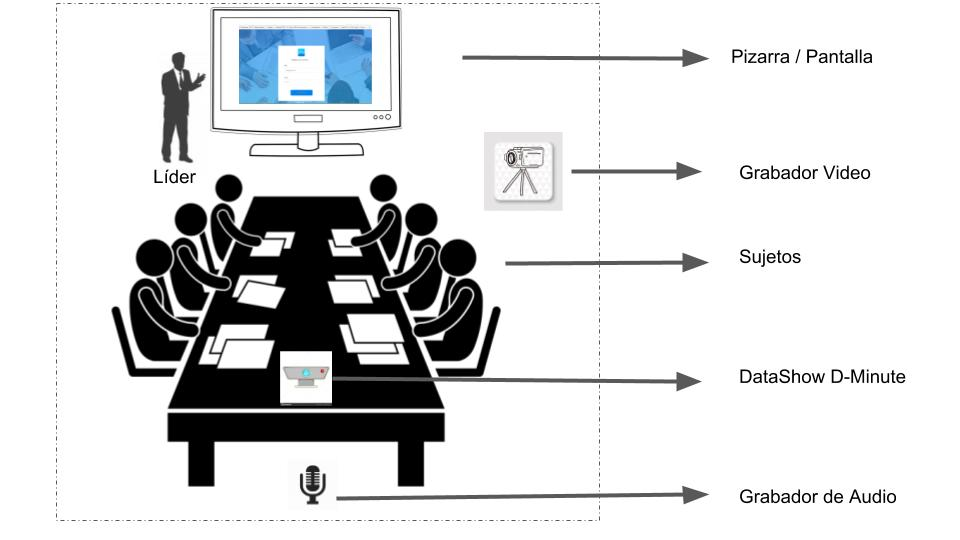
\includegraphics[width=0.8\linewidth]{/setting}
\caption{\textit{Setting} del experimento,  elaboración propia} 
\label{img5-1}
\end{figure}

\subsubsection{Aparato, \textit{software} e instrumento}

Para la captura de datos se requieren instrumentos que nos permitan grabar las sesiones durante el experimento como también el audio de las conversaciones generadas. Ambos en forma separada y con instrumentos diferentes a fin de no perder la calidad para futuros trabajos. 

Otros \textit{software} importantes a considerar es un mezclador de video y voz para unir los datos que se van a capturar de forma separada como también un \textit{software} de transcripción de voz para detectar los actores participantes.

Con el fin de evaluar la circulación de conocimiento se debe utilizar una encuesta del tipo checklist obtenido desde \textit{Knowledge Creation Approach} \fullcite{RN36}. Los resultados serán evaluados en una escala de \textit{Likert}, ver anexo B.

Por último, se requiere de un \textit{notebook} con características básicas para proyectar el \textit{software} de reuniones (D-Minute) del grupo experimental y otro para el grupo de control (actas ofimática) y un proyector. Con las siguientes características recomendadas:

\begin{enumerate}[1.]
	\item Procesador Intel(R) Core 1.3, o superiores
	\item Memoria RAM 4 GB o con mayor capacidad
	\item Disco Duro de 250GB o con 100MB de espacio libre
	\item Tener instalado Java(TM) SE \textit{Runtime Environment} versión 1.8 o superior
	\item Por lo menos una entrada USB 2.0 o mayor
	\item Por lo menos un puerto HDMI

\end{enumerate}

\begin{table}[!h]
\centering
\caption{Alternativas de productos para captura de audio, elaboración propia}
\label{tab:prod31}
\resizebox{15cm}{!} {
\begin{tabular}{|l|c|l|}
\hline
\multicolumn{1}{|c|}{Producto} & \multicolumn{1}{c|}{Precio} & \multicolumn{1}{c|}{URL} \\ \hline
Sennheiser e614 & 219.900 pesos & \url{http://www.centralmusic.cl/microfonos-de-condensador/522-sennheiser-e614-microfono-condensador} \\ \hline
Sennheiser mk8 mic & 609.900 pesos & \url{http://www.centralmusic.cl/microfonos-de-condensador/2939-sennheiser-mk8-mic-condensador} \\ \hline
Rode NT-USB Micrófono Condensador & 149.900 pesos & \url{http://www.centralmusic.cl/microfonos-usb/3348-rode-nt-usb-microfono-condensador} \\ \hline
Voice Tracer DVT7000 (Phillips) & 129 dolares & \url{https://www.philips.com.mx/c-p/DVT7000_00/voice-tracer-captacion-de-sonido-en-360degree} \\ \hline
Business Recorder & 2.990 dólares & \url{http://www.meste.cl/Grabacion_de_Voz/Productos/Grabacion/Business_Recorder___Sala_de_Reuniones/} \\ \hline
Tascam DR 05 & 117.810 pesos & \url{http://davidandjoseph.cl/djcl/tascam-dr-05-grabador-de-audio-portatil} \\ \hline
\end{tabular}
}
\end{table}

\begin{table}[!h]
\centering
\caption{Alternativas de productos para transcribir audio, elaboración propia}
\label{tab:prod2}
\resizebox{15cm}{!} {
\begin{tabular}{|l|c|l|}
\hline
\multicolumn{1}{|c|}{Producto} & \multicolumn{1}{c|}{Precio} & \multicolumn{1}{c|}{URL} \\ \hline
Dragon & 399 euros & \url{https://www.nuance.com/es-es/dragon/transcription-solutions.html} \\ \hline
Trascribe & 20 dolares/año & \url{https://transcribe.wreally.com/account/license/purchase} \\ \hline
\end{tabular}
}
\end{table}

\begin{table}[!h]
\centering
\caption{Alternativas de productos para proyectar video, elaboración propia}
\label{tab:prod3}
\resizebox{15cm}{!} {
\begin{tabular}{|l|c|l|}
\hline
\multicolumn{1}{|c|}{Producto} & \multicolumn{1}{c|}{Precio} & \multicolumn{1}{c|}{URL} \\ \hline
Proyector Nebula & 399.990 pesos & \url{https://ankerstore.cl/proyector-smart-pocket-cinema-nebula-capsule-by-anker?gclid=CjwKCAjw_IPcBRAjEiwAl44QkV-pQoIhQBSny8LK-l9ZFOz0f-HbdhTwqev7sHL9rbWcAmpKSdAO5hoCFUUQAvD_BwE} \\ \hline
Proyector LG & 344.000 pesos & \url{https://www.ebay.com/itm/LG-PH550-Minibeam-LED-Pico-Portable-Projector-with-Built-in-Battery} \\ \hline
\end{tabular}
}
\end{table}

\begin{table}[!h]
\centering
\caption{Alternativas de productos para la captura de video, elaboración propia}
\label{tab:prod4}
\resizebox{15cm}{!} {
\begin{tabular}{|l|c|l|}
\hline
\multicolumn{1}{|c|}{Producto} & \multicolumn{1}{c|}{Precio} & \multicolumn{1}{c|}{URL} \\ \hline
Grabadora Sony & 150.000 pesos & \url{https://store.sony.cl/hdr-cx405/p?idsku=165&utm_source=GooglePLA&sem-la-nb-ss-070218-cl-shopping&gclid=CjwKCAjwrNjcBRA3EiwAIIOvq6_oX5J9igQJ-RzC4BClujEEM2AkQoXZi1Vs4ZV_d9oKafoHvqeNARoC7-UQAvD_BwE} \\ \hline
Grabadora Handycam & 172.000 pesos & \url{http://www.audiomusica.com/catalogo/grabadora-de-video-digital-handycam-q4.html?gclid=CjwKCAjwrNjcBRA3EiwAIIOvq9ZZLl9R9q_CUU7KrQMiQW7vFJxfyDr6ydbuVBzGeNqNEOgVEG7A5xoClr0QAvD_BwE} \\ \hline
\end{tabular}
}
\end{table}

\subsubsection{Procedimiento concreto y aplicación de tarea}

El experimento consiste en trabajar en un proyecto que una vez a la semana y durante cuatro sesiones corridas se revise el avance para dilucidar su estado y a la vez su seguimiento, incluye su planificación futura. Cada tratamiento utilizara un tipo específico de acta. El grupo experimental utilizara el sistema D-Minute y el grupo de control actas en ofimática (versión\textit{ad-hoc}) de forma tal que sea posible observar la recuperación del hilo conversacional de lo tratado en reuniones pasadas mediante el uso de los elementos del diálogo. 

A continuación se presenta un diagrama que entregar una imagen general del flujo del experimento:

\begin{figure}[!h]
\centering
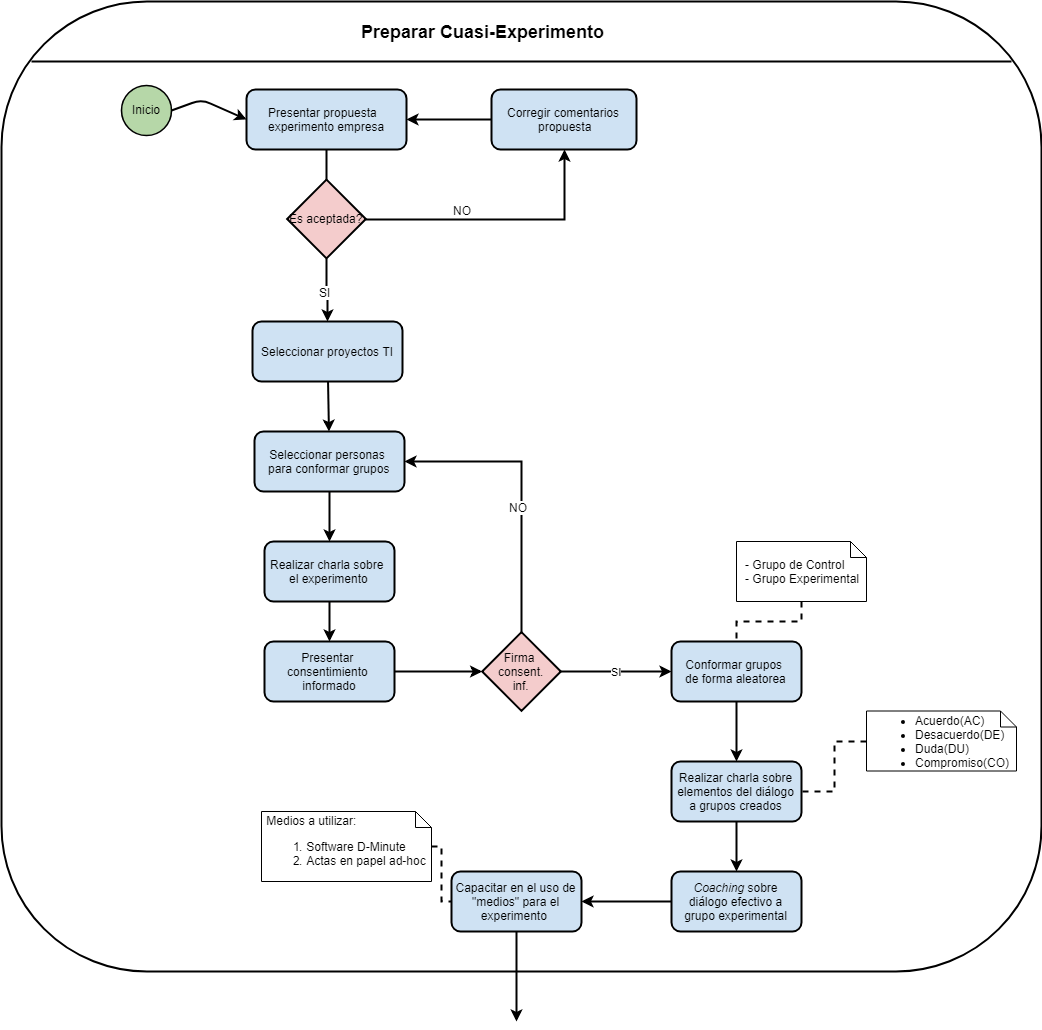
\includegraphics[width=0.8\linewidth]{/datos/recogidadatos-Page-1}
\caption{Flujo preparación del experimento,  elaboración propia} 
\label{img5-2}
\end{figure}

\begin{enumerate}[1.]
	\item Comienza con la presentación de la propuesta a la empresa, y se itera hasta su aprobación.
	\item Se seleccionan los proyectos TI que se van a evaluar.
	\item Se informa a las personas que van a participar sobre el experimento 
	\item Se informa sobre el software y la forma de interacción.
	\item Se solicita firma del consentimiento informado
	\item Se conformar grupos de control y experimental
	\item Se realiza \textit{coaching} al grupo experimental y de control.
	\item Se capacita en el uso de “medios” para realizar el experimento

\begin{figure}[!h]
\centering
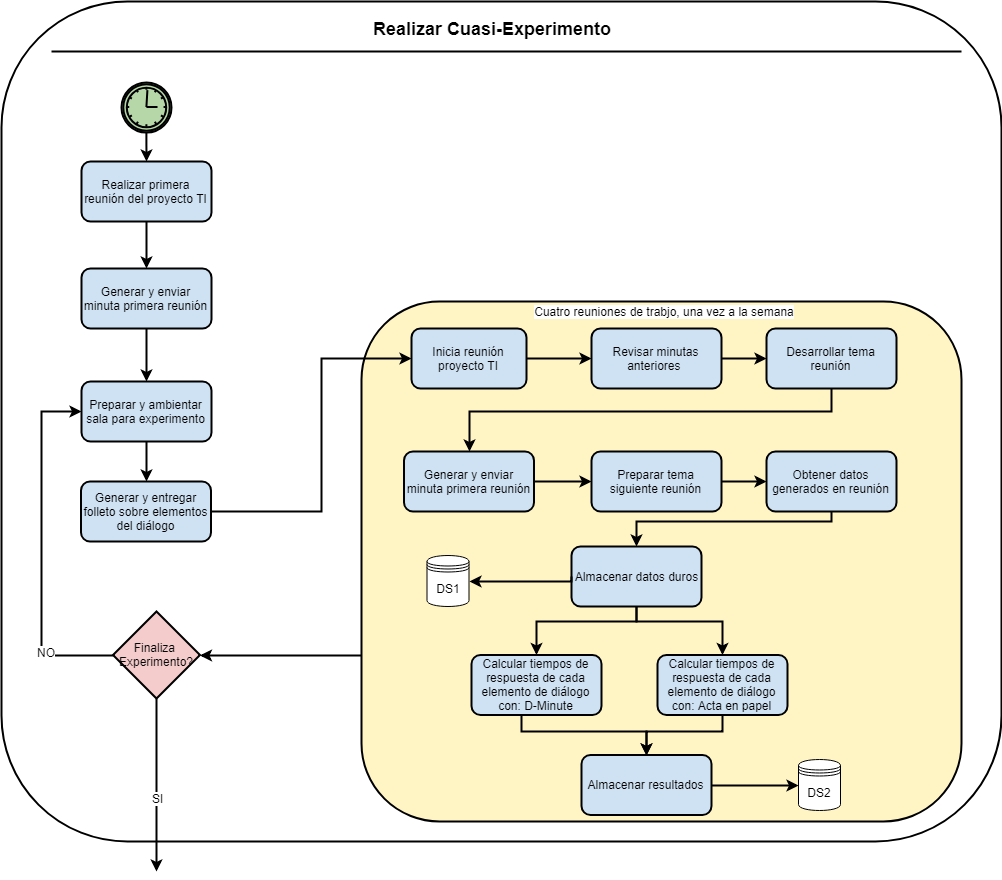
\includegraphics[width=0.8\linewidth]{/datos/recogidadatos-Page-2}
\caption{Flujo realización del experimento,  elaboración propia} 
\label{img5-3}
\end{figure}

	\item Se realiza la primera reunión del proyecto TI, la cual sirve de base para organizar las siguientes tareas del proyecto.
	\item Se prepara el ambiente para las sesiones: proyector, grabador de audio y tríptico sobre elementos del diálogo.
	\item Se inicia el experimento revisando el acta anterior y sus puntos relevantes, se ubican elementos del diálogo.
	\item Se da inicio a los siguientes temas de la reunión, se establecen los elementos del diálogo que puedan haber aparecido y se registran en el medio asignado para ello (D-Minute, actas en papel de ofimática).
	\item Se confecciona acta de la reunión y se envía a cada participante.
	\item Se almacenan los resultados y tiempos que tomó ubicar y establecer cada elemento de diálogo de los medios disponibles para el experimento.

\begin{figure}[!h]
\centering
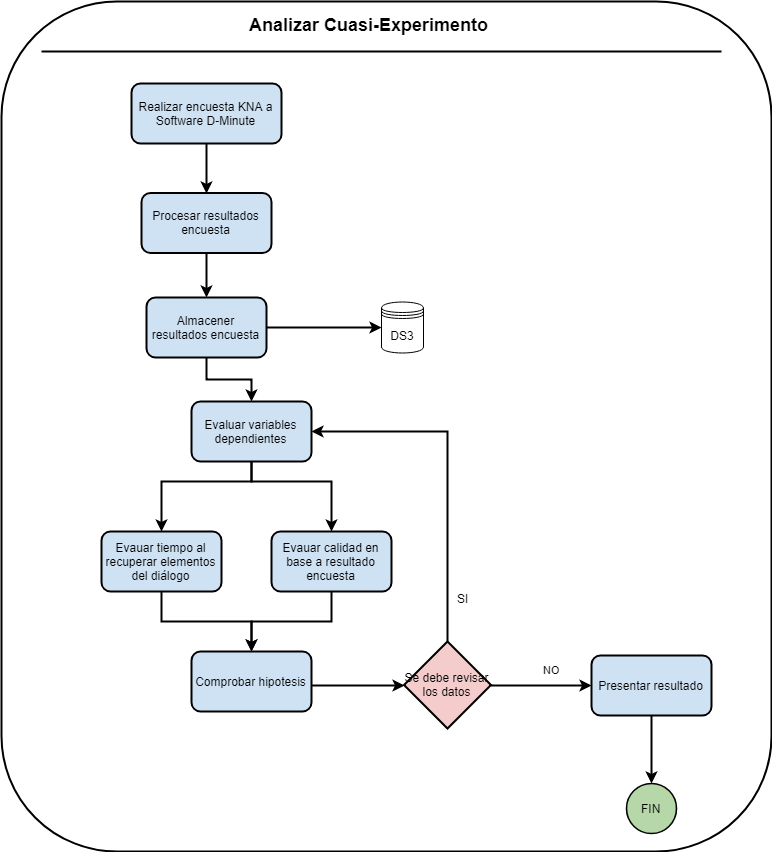
\includegraphics[width=0.8\linewidth]{/datos/recogidadatos-Page-3}
\caption{Flujo análisis del experimento,  elaboración propia} 
\label{img5-4}
\end{figure}

	\item Al finalizar las sesiones del experimento, se procede a realizar una encuesta al grupo experimental sobre la calidad del medio utilizado en el experimento.
	\item Se analizan los datos de manera no presencial y se comprueban los resultados para dar validez de las hipótesis científica.

\end{enumerate}

\subsubsection{Descripción del Dataset a ser generado}

La obtención de los datos es una de las etapas más relevantes dentro del experimento debido a que la información nos permite comprobar las hipótesis planteadas, por lo tanto se debe establecer un dataset adecuado para el conjunto de información esperado. Dado que utilizaremos instrumentos para la captura de audio y la captura de video de ambos grupos del experimento por cada reunión realizada, se propone el siguiente \textit{dataset}, ver tabla \ref{tab:dataset}.

\begin{table}[!h]
\centering
\caption{\textit{Dataset} instrumentos de reunión, elaboración propia}
\label{tab:dataset}
\resizebox{15cm}{!} {
\begin{tabular}{|l|r|l|l|l|l|}
\hline
\multicolumn{1}{|c|}{\textbf{Grupo Experimental}} & \multicolumn{1}{c|}{\textbf{Número Reunión}} & \multicolumn{1}{c|}{\textbf{Video}} & \multicolumn{1}{c|}{\textbf{Audio}} & \multicolumn{1}{c|}{\textbf{Transcripción (texto)}} & \multicolumn{1}{c|}{\textbf{Enlace Reunión (URL)}} \\ \hline
Control & 1 & reunion\_c1.mp4 & reunión\_c1.mp3 & Lorem Ipsum &  \\ \hline
Experimental & 1 & reunion\_e1.mp4 & reunión\_e1.mp3 & Lorem Ipsum &  \\ \hline
 &  &  &  &  &  \\ \hline
\end{tabular}
}
\end{table}

Para determinar nuestras hipótesis es importante determinar el tiempo que cada equipo toma en recuperar los elementos del diálogo de las reuniones pasadas y para esto se propone el siguiente dataset que nos permita recopilar la información a procesar, ver tabla \ref{tab:dataset1}.


\begin{table}[!h]
\centering
\caption{\textit{Dataset} recuperación elementos de diálogo, elaboración propia}
\label{tab:dataset1}
\resizebox{15cm}{!} {
\begin{tabular}{|l|r|l|l|r|l|}
\hline
\multicolumn{1}{|c|}{\textbf{Grupo Experimental}} & \multicolumn{1}{c|}{\textbf{Número Reunión}} & \multicolumn{1}{c|}{\textbf{Elemento de Diálogo}} & \multicolumn{1}{c|}{\textbf{Tiempo de Recuperación}} & \multicolumn{1}{c|}{\textbf{Reunión de Procedencia}} & \multicolumn{1}{c|}{\textbf{Enlace Reunión (URL)}} \\ \hline
Control & 1 & Compromiso & 5 seg. & 2 &  \\ \hline
Experimental & 1 & Duda & 15 seg. & 1 &  \\ \hline
 &  &  &  &  &  \\ \hline
\end{tabular}
}
\end{table}

Por último, si bien nuestro mayor valor es determinar el tiempo que toma cada persona en recuperar el hilo conversacional de las reuniones pasadas. Es importante determinar la circulación de conocimiento que ocurre dentro de D-Minute, para esto se requiere un dataset que nos permita recopilar las encuestas KNA (ver anexo B) aplicadas a cada sujeto que asiste a la reunión, ver tabla \ref{tab:dataset2}.

\begin{table}[!h]
\centering
\caption{\textit{Dataset} encuesta KNA para D-Minute, elaboración propia}
\label{tab:dataset2}
\resizebox{15cm}{!} {
\begin{tabular}{|l|r|l|r|l|}
\hline
\multicolumn{1}{|c|}{\textbf{Grupo Experimental}} & \multicolumn{1}{c|}{\textbf{Número Reunión}} & \multicolumn{1}{c|}{\textbf{Asistente Encuestado}} & \multicolumn{1}{c|}{\textbf{Nota Encuesta}} & \multicolumn{1}{c|}{\textbf{Enlace Reunión (URL)}} \\ \hline
Control & 1 & Oliver Hidalgo & 70 &  \\ \hline
Experimental & 1 & Juan Fuenzalida & 15 &  \\ \hline
 &  &  &  &  \\ \hline
\end{tabular}
}
\end{table}

\subsubsection{Análisis estadístico propuesto}

Para evaluar nuestras hipótesis del experimento expuesto se plantea la aplicación de diversos test estadísticos a las variables independientes descritas en las secciones anteriores. Estos test de hipótesis tendrán la finalidad de encontrar diferencias significativas en los resultados obtenidos. por tanto para determinar $\mathrm{H_{Tiempo}}$ se sugiere la aplicación de test del tipo t de student, ANOVA. Se recuerda que estos análisis son sugeridos y pueden variar al momento de definir con mayor claridad la aplicación del experimento. 

Para la circulación de conocimiento la cual es nuestra segunda hipótesis $\mathrm{H_{Conocimiento}}$, se sugiere aplicar escala de \textit{likert} a las encuestas realizadas y calcular el promedio por reunión y por grupo de control a fin de determinar nuestra hipótesis.

\subsection{RESUMEN}

El presente capítulo expuso el diseño experimental de la investigación que debe ser ejecutado para una evaluación de la herramienta D-Minute. En la primera sección se dan detalles del contexto de investigación mostrando las preguntas, variables e hipótesis que guían el estudio. Luego, la siguiente sección presenta el diseño detallado del experimento pasando por cada etapa del experimento. 

En el próximo capítulo se presentan las conclusiones del estudio presentado y los siguientes pasos.

%Falta diseño del experimento aqui
\section{CONCLUSIONES}

El siguiente capítulo expone las conclusiones de este trabajo de tesis - cuyo mínimo producto viable fue D-Minute - pasando por la investigación, el desarrollo y una pequeña parte de innovación I+D+i. De lo anterior se puede indicar que se va recapitular los contenidos del capítulo primero para concluir en base los objetivos planteados; como fueron realizados y en qué forma se llevaron a cabo. Luego, se proponen los alcances producto de la ejecución para indicar los trabajos futuros que se deben seguir con el objeto de avanzar en el estudio. Finalmente se presenta una reflexión personal acerca del trabajo.


\subsection{OBJETIVOS}

En la sección 1.4.2 de este documento se presentan los objetivos específicos que deben ser llevados a cabo para lograr el objetivo general del proyecto. En base a estos se elabora las siguientes conclusiones de cada unos de ellos:

\subsubsection{Objetivo específicos}

\textit{OBJETIVO 1:  “Hacer una revisión de la literatura de los \textit{meetingware} con sus características para relacionarlo con D-Minute"}\newline

Se logra el objetivo planteado el cual puede verse en detalle en el capítulo dos del mismo documento así como sus correspondientes fuentes bibliográficas. Se indican algunos de los principales \textit{software} de reuniones que poseen una base científica y de lo anterior se logra establecer el marco de investigación.\newline

\textit{OBJETIVO 2:  “Comparar D-Minute con otros \textit{meetingware} en términos comerciales"}\newline

Se logra el objetivo planteado el cual puede verse en detalle en el capítulo tres, se exponen diferentes \textit{meetingare} comerciales algunos de ellos muy exitosos. De esta información se genera un \textit{benchmarking} del producto, realizando una comparación con los criterios de evaluación detectados tanto en la revisión bibliográfica como en la revisión de mercado sobre lo que es necesario en un \textit{software} de reuniones.\newline

\textit{OBJETIVO 3:  “Dise\~nar una propuesta de valor de D-Minute cómo \textit{meetingware} tendiente a convertirse en una potencial innovación en el mercado"}\newline

Se logra el objetivo planteado el cual puede verse en detalle en el capítulo tres donde se expone el lienzo de canvas D-Minute desarrollado con metodología Lean Startup. La formulación de la idea nace de la revisión de mercado expuesta en el mismo capítulo cuyo primer objetivo es entregar una herramienta al mercado que posea una síntesis dialógica como pilar para la recuperación del contexto como medio para tener reuniones efectivas.\newline

\textit{OBJETIVO 4:  “Desarrollar el artefacto de \textit{software} D-Minute con el principio de las actas dialógicas que permita administrar reuniones con los elementos del diálogo y las tareas asociadas"}\newline

Se logra el objetivo planteado el cual puede verse en detalle en el capítulo cuatro. El desarrollo del \textit{software} tuvo dos enfoques: en primer lugar conocer la opinión  - mediantes encuestas realizadas - de diferentes gestores de proyecto de empresas como Banco BCI, Caja Los Andes, Comder y Banco de Chile sobre los criterios que debe incluir un sistema de este tipo. En segundo lugar la incorporación de la síntesis dialógica en herramientas de reuniones, no solamente el compromiso sino el resto de elementos (dudas, desacuerdos, acuerdo, norma común, acuerdos de coordinación y tarea) que se pasan por alto en estas instancias.\newline

\textit{OBJETIVO 5:  “Dise\~nar una validación de D-Minute por medio de una investigación científica para mostrar las ventajas en tiempos y en circulación del conocimiento2}\newline

Se logra el objetivo planteado el cual puede verse expuesto en el capítulo cinco. Se presenta el diseño del experimento, como debe ser ejecutado, la recolección de datos y lo necesario para que el experimento puede ser ejecutado en otro estudio.

\subsubsection{Objetivo general}

\textit{OBJETIVO GENERAL: “Desarrollar un tipo actas de reuniones que facilite la recuperación, el estado de reuniones pasadas y el flujo del conocimiento basada en el enfoque diálogo/acción"}\newline

En base a los objetivos específicos cumplidos en su mayoría y apoyada por la información expuesta en este mismo documento, se ha cumplido el objetivo general de la tesis. D-Minute es un \textit{software} del área de los meetingware que fue desarrollado con tecnología de vanguardia, se aloja en un servidor PaaS y posee la teoría del diálogo para el seguimiento de reuniones. 

\subsection{CONCLUSIONES GENERALES}

El desarrollo de esta tesis estuvo ligada tanto a la investigación como al desarrollo, pero sin embargo pudimos incorporar una linea mas pequeña. La innovación, que sin duda aporta un tremendo valor cuando se combina con investigación y desarrollo pues podemos ver como una idea empieza a tomar forma al punto de contribuir a la sociedad.

La investigación realizada expuso la diversidad de sistemas que existen en el área de meetingware y como cada uno de ellos ha contribuido al apoyo de las personas a lo largo de los años, debido a que las reuniones son la forma de coordinar el trabajo colaborativo. Además, el desarrollo de la aplicación fue utilizando la tendencia del mercado, el uso de micro arquitectura para la creación de \textit{software} permite mayor velocidad en los desarrollos, escalabilidad y \textit{performance} que mezclada con PaaS logra una alta disponibilidad del producto.

Se emplearon dos metodologías para la creación del producto como del modelo de negocio. Scrum para el desarrollo de \textit{software} que permitió lograr el MVP pues en cada iteración se dio foco a las principales funciones y no al todo del producto. Por otra parte, para el desarrollo del modelo liviano de negocio se utilizó Lean Startup que permitió descubrir a qué mercado estaría enfocado el producto como los clientes finales del mismo.

Finalmente y dado que los objetivos se dan por cumplidos, durante la revisión bibliográficas se presentaron dos preguntas de investigación de mercado a responder:

\begin{enumerate}[1.]
	\item ¿D-Minute expone los elementos de diálogo mejor que otras herramientas síncronas?

R: En base al cuadro comparativo realizado en el capítulo tres, D-Minute expone todos los elementos de diálogo, genera una trazabilidad de los elementos y permite un seguimiento de ellos.

	\item ¿Qué ventaja competitiva posee D-Minute respecto a los productos comerciales existentes hoy día en el mercado?

R: Además de los diferentes elementos de diálogo que emplea D-Minute, a diferencia de sus competidores que solo utilizan los compromisos la gestión del proyecto. D-Minute ofrece un seguimiento de tareas para los compromisos y es una plataforma que opera bajo el concepto de simple en términos de usabilidad.

\end{enumerate}

\subsection{ALCANCES}

Las conclusiones del trabajo realizado se aplican principalmente al desarrollo de una aplicación y su respectivo diseño comparativo. Por tanto se espera que lo observado en el documento sea generalizable a meetingware que utilicen la síntesis dialógica dentro de sus bases. 

\subsection{TRABAJOS FUTUROS}

Si bien el trabajo cumple con los objetivos planteados en el tiempo disponible para ser ejecutado. Deja muchos espacios de mejora que pueden ser abordados en futuros trabajos para concluir la investigación:

\begin{enumerate}[1.]
	\item Capacidad de generar un complemento para obtener la agenda del gestor. Esto sería de gran valor pues habría información pre-cargada como por ejemplo: fecha y hora de reunión, asistentes y descripción, lo cual permitiría a cada usuario completar la información en vez de crearla en dos sistemas.
	\item Generar \textit{login} con una cuenta de redes sociales u alguna corporativa para evitar múltiples claves de sistemas.
	\item Capacidad de adjuntar documentos relevantes tanto en la reunión ejecutada como en el proyecto con el fin de disponer información a los participantes.
	\item Generar recordatorios de las tareas asociadas a los compromisos adquiridos en las reuniones utilizando la fecha de entrega y el estado como parámetro de seguimiento. 
	\item Generar una versión \textit{responsive} para IOS y Android pues hoy en día la tendencia es a utilizar celulares para el seguimiento de temas. Lo que podría permitir mayor adaptación de la herramienta como medio para reuniones efectivas.
	\item Probar científicamente que D-Minute permite recuperar el contexto de reuniones pasadas utilizando la teoría del diálogo. 
	\item Publicar los resultados del punto seis en un artículo científico para generar nuevas investigaciones de la teoría del diálogo en reuniones de trabajo.

\end{enumerate}

\subsection{REFLEXION PERSONAL}

Este trabajo se ideó como una forma de contribuir en la línea de \textit{meetingware}; sin embargo y personalmente dejo mucho mas que eso, pues siempre queremos enfocar hacia donde deben ir las personas con nuestros sistemas pero al revés es algo distinto. Desde una forma de comunicación diseñar un software que permita las personas usar el recurso más valioso que hoy tenemos es sin duda un trabajo gigantesco. El tiempo es lo que más cuidamos y estar en reuniones que no aportan valor, pues al menos la mitad del tiempo estamos entregando contexto de lo revisado anteriormente, genera un desgaste en diversos aspectos.

La teoría del diálogo es algo nuevo tanto para el alumno como para muchas personas, debemos tender a una nueva forma de abordar los problemas a través de la comunicación  efectiva. Que en un contexto de reuniones pasar a ser muy efectiva si lo que buscamos es que la otra persona me entienda. Por estas razones este trabajo no solo trajo consigo la elaboración de un documento sino descubrir una forma emplear el diálogo en contextos de conversación.

Finalmente, los trabajos de investigación estuvieron muy ligados al desarrollo de nuevas tendencias en la industria del \textit{software}, las nuevas tecnologías tomadas en este trabajo dejan una base potente para los trabajos futuros que desean aportar conocimiento sobre la línea de meetingware u otra.






%----------------------------------------------------------------------------------------
%	BIBLIOGRAPHY
%----------------------------------------------------------------------------------------
\bibliography{TesisMagister}
\nocite{*}

%ANEXOS
\appendix
\clearpage
\addappheadtotoc
\appendixpage
\section{Encuesta criterios de evaluación y resultado}

El presente anexo es el resultado de la aplicación de la encuesta: criterio para un software de reuniones, sobre la cual se hizo el \textit{Benchmark} de las herramientas \textit{meetingware} y programas similares que compiten con D-Minute. Dicha encuesta fue aplicada a gestores de proyecto que a diario se ven enfrentados a reuniones de proyecto para coordinar su trabajo.

A continuación, se muestra la encuesta realizada y sus resultados por criterio. Los cuales fueron la base para preparar el capitulo 3. 

\begin{figure}[h]
\centering
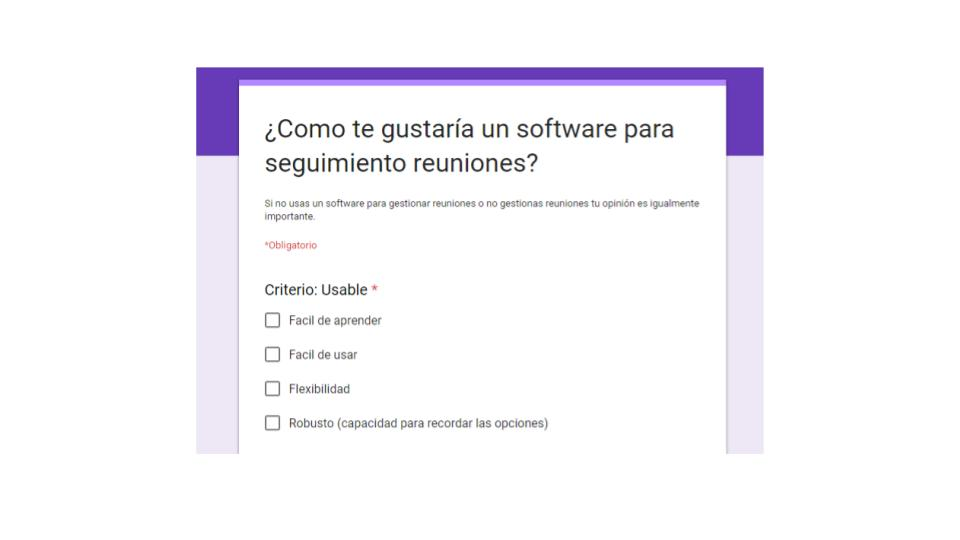
\includegraphics[width=0.8\linewidth]{/encuesta1}
\end{figure}

\begin{figure}[h]
\centering
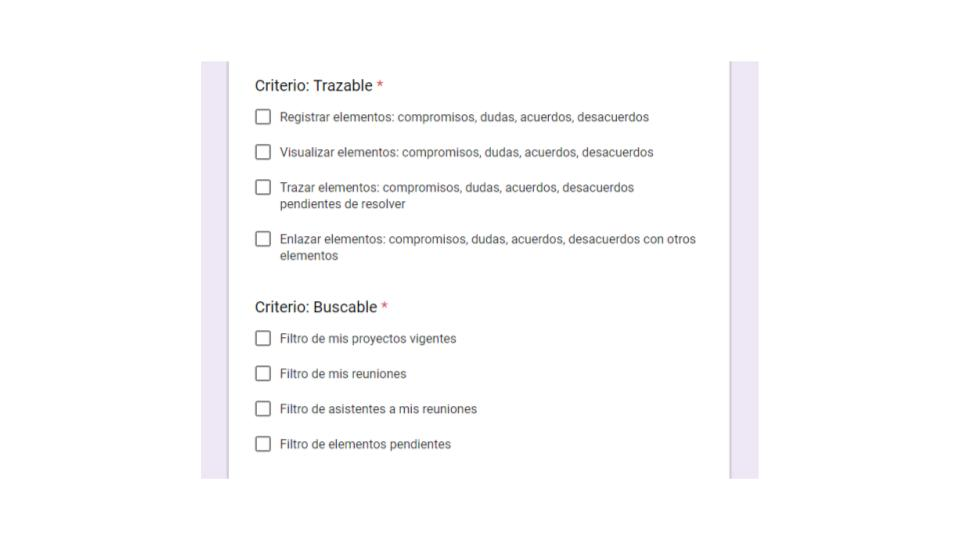
\includegraphics[width=0.8\linewidth]{/encuesta2}
\end{figure}

\begin{figure}[h]
\centering
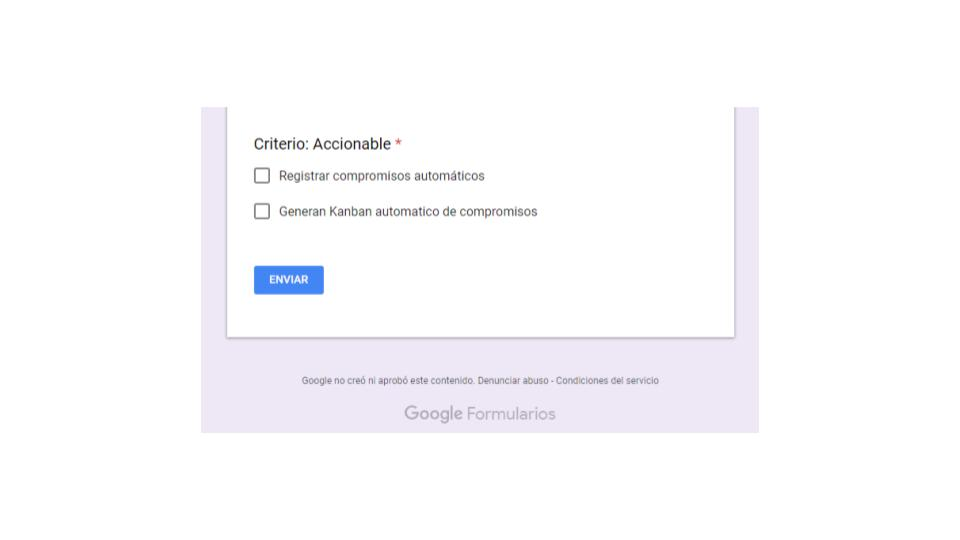
\includegraphics[width=0.8\linewidth]{/encuesta3}
\end{figure}

\begin{figure}[h]
\centering
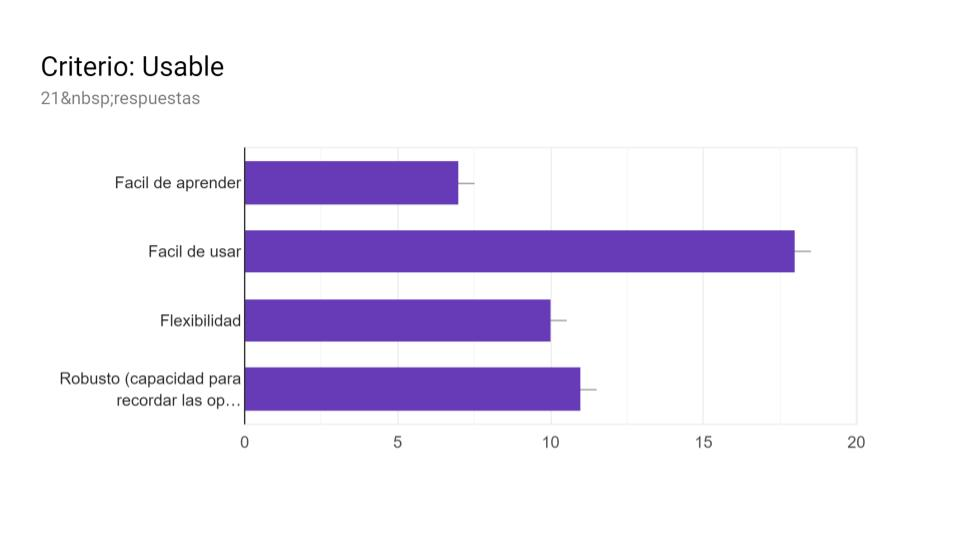
\includegraphics[width=0.8\linewidth]{/resultado1}
\end{figure}

\begin{figure}[h]
\centering
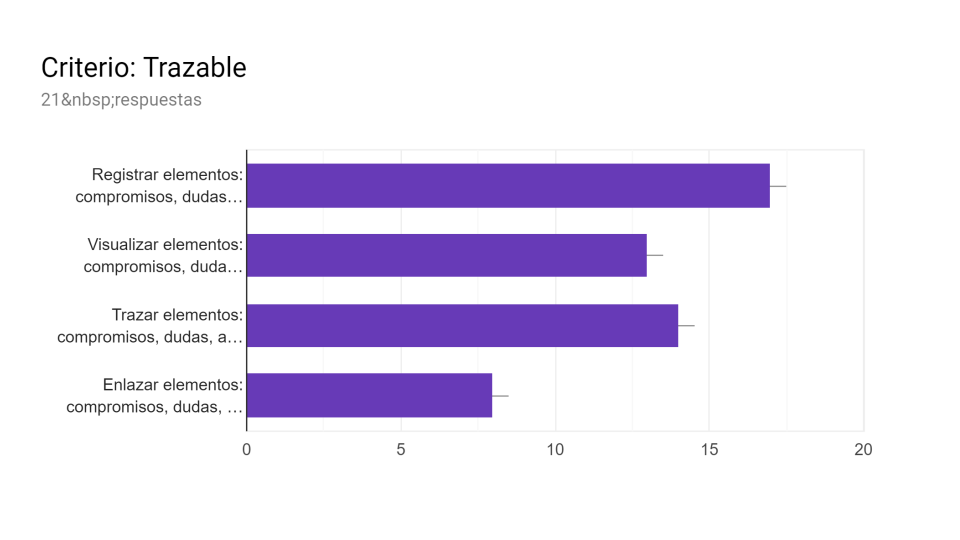
\includegraphics[width=0.8\linewidth]{/resultado2}
\end{figure}

\begin{figure}[h]
\centering
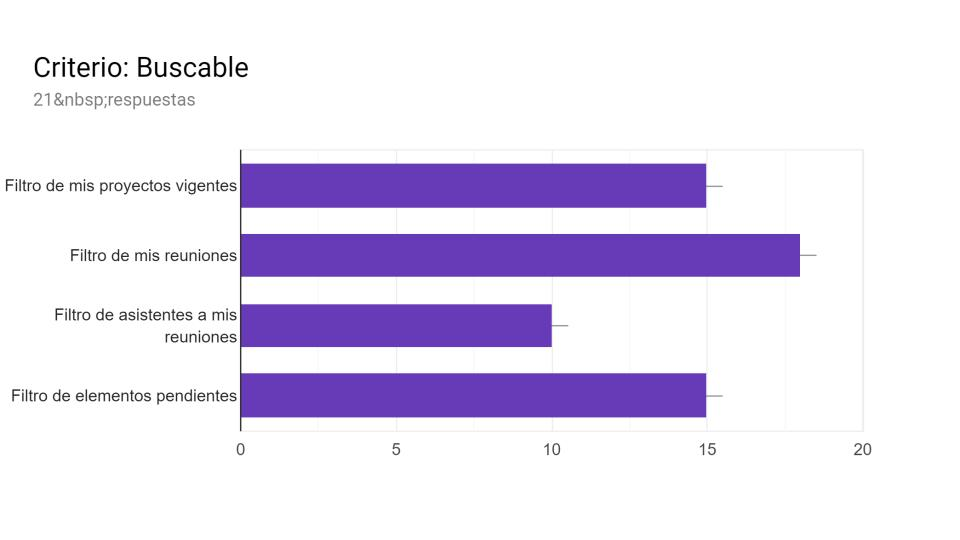
\includegraphics[width=0.8\linewidth]{/resultado3}
\end{figure}

\begin{figure}[h]
\centering
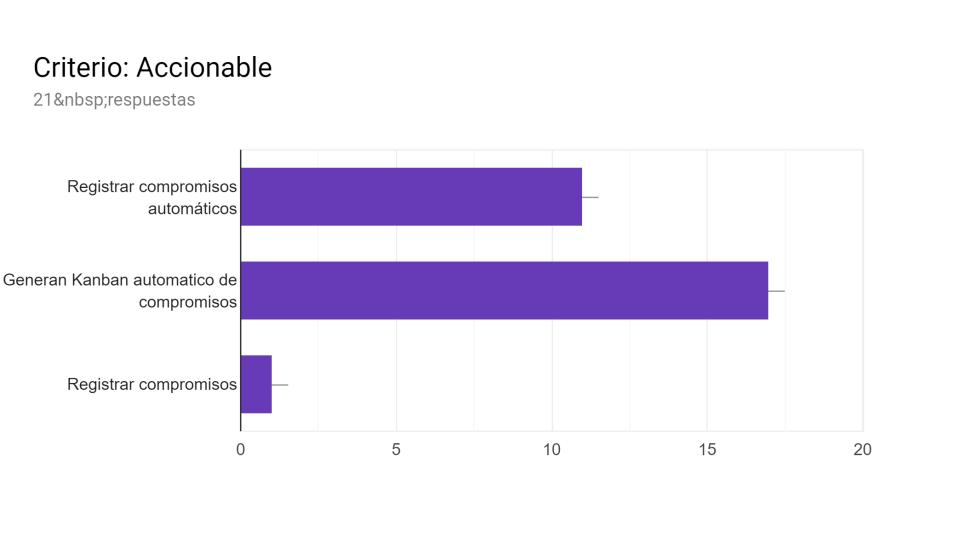
\includegraphics[width=0.8\linewidth]{/resultado4}
\end{figure}

\section{Encuesta KNA}

Checklist “Evaluación de Aplicaciones Colaborativas desde la aproximación de la Administración del Conocimiento”\newline

Basado en el artículo: Evaluating Collaborative Applications from a Knowledge Management Approach, Aurora Vizcaíno, Manuel Martínez, Gabriela Aranda, Mario Piattini, University of Castilla-La Mancha, Escuela Superior de Informática, España.\newline

Encuesta de Calidad para la Herramienta: \underline{            }

\begin{enumerate}[1.]
    \item Creación de conocimiento
    
\begin{table}[!h]
\centering
\resizebox{15cm}{!} {
\begin{tabular}{|l|r|l|r|l|l|}
\hline
\multicolumn{1}{|c|}{\textbf{}} & \multicolumn{1}{c|}{\textbf{Nunca}} & \multicolumn{1}{c|}{\textbf{Rara Vez}} & \multicolumn{1}{c|}{\textbf{A Veces}} & \textbf{Frecuentemente} & \multicolumn{1}{c|}{\textbf{Siempre}} \\ \hline
\begin{tabular}[c]{@{}l@{}}a.- ¿La herramienta ayuda a encontrar la información que busca?, \\ ¿El sistema ayuda a entenderla?,  \\ Por ejemplo, ¿el sistema muestra ejemplos para aclarar los conceptos?\end{tabular} &  &  &  &  &  \\ \hline
b.- ¿El sistema propone soluciones a los problemas? &  &  &  &  &  \\ \hline
c.- ¿Tiene la herramienta algún mecanismo para explicar las soluciones que muestra? &  &  &  &  &  \\ \hline
\end{tabular}
}
\end{table}    
    
    \item Acumulación de conocimiento
    
\begin{table}[!h]
\centering
\resizebox{15cm}{!} {
\begin{tabular}{|l|r|l|r|l|l|}
\hline
\multicolumn{1}{|c|}{\textbf{}} & \multicolumn{1}{c|}{\textbf{Nunca}} & \multicolumn{1}{c|}{\textbf{Rara Vez}} & \multicolumn{1}{c|}{\textbf{A Veces}} & \textbf{Frecuentemente} & \multicolumn{1}{c|}{\textbf{Siempre}} \\ \hline
\begin{tabular}[c]{@{}l@{}}a.-¿ La herramienta tiene un repositorio donde la información se pueda almacenar?,\\ ¿Esta base de datos tiene suficiente calidad?\end{tabular} &  &  &  &  &  \\ \hline
b.- ¿La herramienta tiene mecanismos inteligentes para capturar la información? &  &  &  &  &  \\ \hline
c.- ¿La herramienta ayuda a documentar las actividades diarias? &  &  &  &  &  \\ \hline
\end{tabular}
}
\end{table}     
    
    \item Compartir conocimiento
    
\begin{table}[!h]
\centering
\resizebox{15cm}{!} {
\begin{tabular}{|l|l|l|l|l|l|}
\hline
\multicolumn{1}{|c|}{\textbf{}} & \multicolumn{1}{c|}{\textbf{Nunca}} & \multicolumn{1}{c|}{\textbf{Rara Vez}} & \multicolumn{1}{c|}{\textbf{A Veces}} & \textbf{Frecuentemente} & \multicolumn{1}{c|}{\textbf{Siempre}} \\ \hline
\begin{tabular}[c]{@{}l@{}}a.- ¿La herramienta tiene mecanismos para comunicarse con otras personas?, \\ ¿Qué mecanismos tiene: síncrono (chat, videoconferencia, pizarras compartidas), \\ asíncrono (email, listas de mail, grupos de noticias, foros asíncronos)?\end{tabular} & \multicolumn{1}{r|}{} &  & \multicolumn{1}{r|}{} &  &  \\ \hline
b.- ¿La herramienta tiene mecanismos para ubicar a expertos? & \multicolumn{1}{r|}{} &  & \multicolumn{1}{r|}{} &  &  \\ \hline
c.- ¿Tiene la herramienta algún mecanismo para explicar las soluciones que muestra? & \multicolumn{1}{r|}{} &  & \multicolumn{1}{r|}{} &  &  \\ \hline
d.- ¿La herramienta tiene mecanismos para rastrear el trabajo de estas comunidades de práctica? &  &  &  &  &  \\ \hline
\begin{tabular}[c]{@{}l@{}}e.- ¿El sistema tiene un mecanismo para enviar nueva información a aquellos \\ miembros del equipo que podrían necesitarla?\end{tabular} &  &  &  &  &  \\ \hline
f.- ¿La herramienta tiene control de flujos de trabajo? &  &  &  &  &  \\ \hline
\begin{tabular}[c]{@{}l@{}}g.- ¿La herramienta tiene mecanismos para detectar que persona puede saber sobre un tema \\ o información que otra persona necesite?\end{tabular} &  &  &  &  &  \\ \hline
\end{tabular}
}
\end{table}    
    
    \item Utilización de conocimiento
    
\begin{table}[!h]
\centering
\resizebox{15cm}{!} {
\begin{tabular}{|l|r|l|r|l|l|}
\hline
\multicolumn{1}{|c|}{\textbf{}} & \multicolumn{1}{c|}{\textbf{Nunca}} & \multicolumn{1}{c|}{\textbf{Rara Vez}} & \multicolumn{1}{c|}{\textbf{A Veces}} & \textbf{Frecuentemente} & \multicolumn{1}{c|}{\textbf{Siempre}} \\ \hline
a.- El sistema tiene métodos para buscar o filtrar información? &  &  &  &  &  \\ \hline
b.- ¿El sistema tiene técnicas para evitar ruido en la información? &  &  &  &  &  \\ \hline
\begin{tabular}[c]{@{}l@{}}c.- ¿El sistema tiene mecanismos de alerta para aconsejar al usuario para \\ consultar información o contactar a otras personas?\end{tabular} &  &  &  &  &  \\ \hline
d.- ¿El sistema recomienda la mejor forma de llevar a cabo una tarea? & \multicolumn{1}{l|}{} &  & \multicolumn{1}{l|}{} &  &  \\ \hline
\end{tabular}
}
\end{table}      
    
    \item Internalización del Conocimiento
    
\begin{table}[!h]
\centering
\resizebox{15cm}{!} {
\begin{tabular}{|l|r|l|r|l|l|}
\hline
\multicolumn{1}{|c|}{\textbf{}} & \multicolumn{1}{c|}{\textbf{Nunca}} & \multicolumn{1}{c|}{\textbf{Rara Vez}} & \multicolumn{1}{c|}{\textbf{A Veces}} & \textbf{Frecuentemente} & \multicolumn{1}{c|}{\textbf{Siempre}} \\ \hline
a.- ¿El sistema ayuda a aprender cómo llevar a cabo una tarea? &  &  &  &  &  \\ \hline
b.- ¿El sistema tiene un mecanismo para mejorar las habilidades del empleado? &  &  &  &  &  \\ \hline
\begin{tabular}[c]{@{}l@{}}c.- ¿El sistema tiene técnicas para enseñar filosofía organizacional, estándares,\\  y perfiles de clientes?\end{tabular} &  &  &  &  &  \\ \hline
\end{tabular}
}
\end{table}     
    
    \item Integración de conocimiento
    
\begin{table}[!h]
\centering
\resizebox{15cm}{!} {
\begin{tabular}{|l|r|l|r|l|l|}
\hline
\multicolumn{1}{|c|}{\textbf{}} & \multicolumn{1}{c|}{\textbf{Nunca}} & \multicolumn{1}{c|}{\textbf{Rara Vez}} & \multicolumn{1}{c|}{\textbf{A Veces}} & \textbf{Frecuentemente} & \multicolumn{1}{c|}{\textbf{Siempre}} \\ \hline
a.- ¿El sistema facilita la integración de información y conocimiento? &  &  &  &  &  \\ \hline
\end{tabular}
}
\end{table}        
\end{enumerate}
\section{Desarrollo completo del producto}

En esta sección podrá encontrar el paso a paso de la solución de \textit{software} D-Minute y la forma que fue abordado en cada \textit{sprint}.

\subsection{Github}

Para el almacenamiento de código fuente se utilizó GitHub, los repositorios que se muestran a continuación tienen la versión instalada en producción:

\begin{table}[!h]
\centering
\resizebox{15cm}{!} {
\begin{tabular}{|l|c|c|l|}
\hline
\multicolumn{1}{|c|}{\textbf{Repositorio}} & \textbf{Tipo} & \textbf{Lenguaje} & \multicolumn{1}{c|}{\textbf{Comentario}} \\ \hline
https://github.com/woliverhl/d-minute-front.git & Front-End & Angular 5 & Versión Front de la aplicación \\ \hline
https://github.com/woliverhl/config-server-dminute.git & Configuración & YML & Contiene los archivos de configuración \\ \hline
https://github.com/woliverhl/d-minute-ms.git & Back-End & Java 1.8 & Versión Back-End de la aplicación \\ \hline
https://github.com/woliverhl/d-minute-zuul.git & \multicolumn{1}{l|}{Zuul} & \multicolumn{1}{l|}{Java 1.8} & Proxy de la aplicación \\ \hline
https://github.com/woliverhl/d-minute-eureka.git & \multicolumn{1}{l|}{Eukera} & \multicolumn{1}{l|}{Java 1.8} & Almacena los microservicios \\ \hline
https://github.com/woliverhl/d-minute-config-server.git & \multicolumn{1}{l|}{Config-Server} & \multicolumn{1}{l|}{Java 1.8} & Entrega la configuración de los servicios \\ \hline
\end{tabular}
}
\end{table}    

\subsection{Dockerhub}

Dado que se utilizó arquitectura digital para el desarrollo de la solución, las imágenes generadas por cada proyecto descrito anteriormente fueron almacenadas en dockerhub, en los siguientes repositorios:


\begin{table}[!h]
\centering
\resizebox{15cm}{!} {
\begin{tabular}{|l|c|l|}
\hline
\multicolumn{1}{|c|}{\textbf{Repositorio}} & \textbf{Tipo} & \multicolumn{1}{c|}{\textbf{Comentario}} \\ \hline
docker pull ohidalgoleal/d-minute-front & Front-End & Contiene la imagen del front-end productivo \\ \hline
docker pull ohidalgoleal/d-minute-ms & Back-End & Contiene la imagen del back-end productivo \\ \hline
docker pull ohidalgoleal/d-minute-zuul & Zuul & Contiene la imagen del proxy productivo \\ \hline
docker pull ohidalgoleal/d-minute-eureka & Eukera & Contiene la imagen de eureka productivo \\ \hline
docker pull ohidalgoleal/d-minute-config-server & Config-Server & Contiene imagen del servidor de configuración \\ \hline
\end{tabular}
}
\end{table} 

\subsection{Detalle de \textit{Sprint}}

\begin{itemize}
	\item \textbf{\textit{Sprint} 1:} Configurar ambientes para desarrollo.

\begin{itemize}
\item \textit{Spring Backlog}

\begin{table}[!h]
\centering
\label{tab:backlog1}
\begin{tabular}{|l|l|r|}
\hline
\multicolumn{1}{|c|}{\textit{\textbf{Feature}}} & \textbf{Epica} & \textbf{Peso} \\ \hline
Configuración ambiente DMinute & Técnica & 3 \\ \hline
Levantar aplicación web en Heroku & Técnica & 3 \\ \hline
Refactorización de código para creación de temas de la reunión & Técnica & 8 \\ \hline
\end{tabular}
\end{table}

\item Desarrollo: Este \textit{sprint} fue completamente técnico, en primera instancia se configuró el ambiente de desarrollo que nos permitió realizar las primeras líneas de código de la aplicación posteriormente se comenzó a realizar pruebas de concepto con el PaaS de Heroku con resultados satisfactorios, desplegando un servicio “demo”. Por último, una historia de usuario consistía en crear el modelo de datos de un acta de reunión que pudiera soportar los elementos de diálogo y sus respectivos temas.

\item \textit{Spring Review}: Como el \textit{sprint} era netamente técnico no hubo resultados que mostrar al PO, sin embargo se presentó los resultado del modelo de datos (ver figura C1) y el PaaS para desplegar los futuros microservicios.

\begin{figure}[!h]
\centering
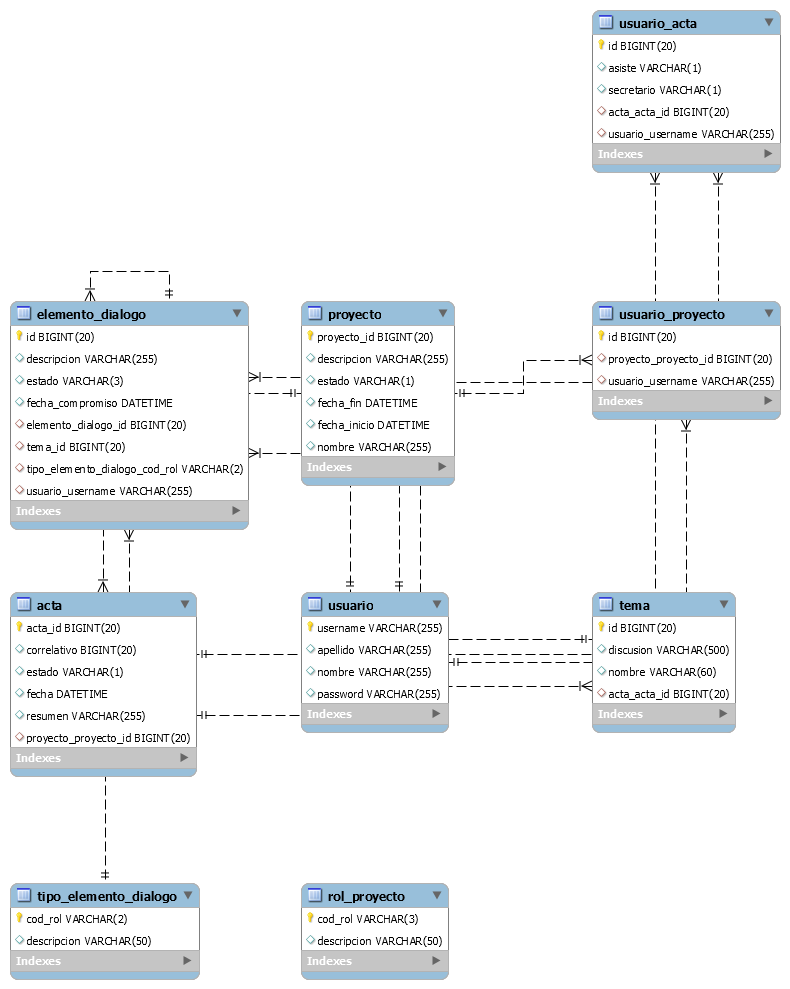
\includegraphics[width=0.7\linewidth]{/modelodminute}
\label{imga-c1}
\caption{Modelo datos crear acta, elaboración propia}
\end{figure}

\end{itemize}


	\item \textbf{\textit{Sprint} 2:} Desarrollar APIs de servicios para la creación de actas y elementos de diálogo.

\begin{itemize}
\item \textit{Spring Backlog}

\begin{table}[!h]
\centering
\label{tab:backlog2}
\begin{tabular}{|l|l|r|}
\hline
\multicolumn{1}{|c|}{\textit{\textbf{Feature}}} & \textbf{Epica} & \textbf{Peso} \\ \hline
Refactorización de código para creación elementos de diálogo & Técnica & 8 \\ \hline
Refactorización de código para creación de minutas & Técnica & 8 \\ \hline
\end{tabular}
\end{table}

\item Desarrollo: Como se indicó en el punto anterior, la aplicación tenía que ser reconstruida, por tanto en este \textit{sprint} se trabajó en migrar el código desarrollado en python a su nueva estructura de java con microservicios. Un trabajo muy complicado que estuvo hasta el último minuto de no ser logrado pues había que estudiar python para ir traspasando las funciones del proyecto al nuevo lenguaje java. Esta tarea se tornó compleja dada la complejidad de manejar ambos lenguajes, pero el trabajo colaborativo permitió crear la sección de minutas y elementos de diálogo como API,s desplegar en heroku para ser utilizadas en los próximos \textit{sprint}. Respecto a la base datos, se estuvo trabajando tanto en la creación de las tablas como en su configuración en la nube con el objetivo de entregar las primeras API`s del servicio.

\item \textit{Spring Review}: Para esta review era importante mostrar software funcionando sin embargo y dado que la parte front-end era muy pesada de construir en términos de puntos. Se presentaron las APIs construidas utilizando postmand\footnote{Definición en: \url{https://www.getpostman.com/}} (ver figura C2).

\begin{figure}[!h]
\centering
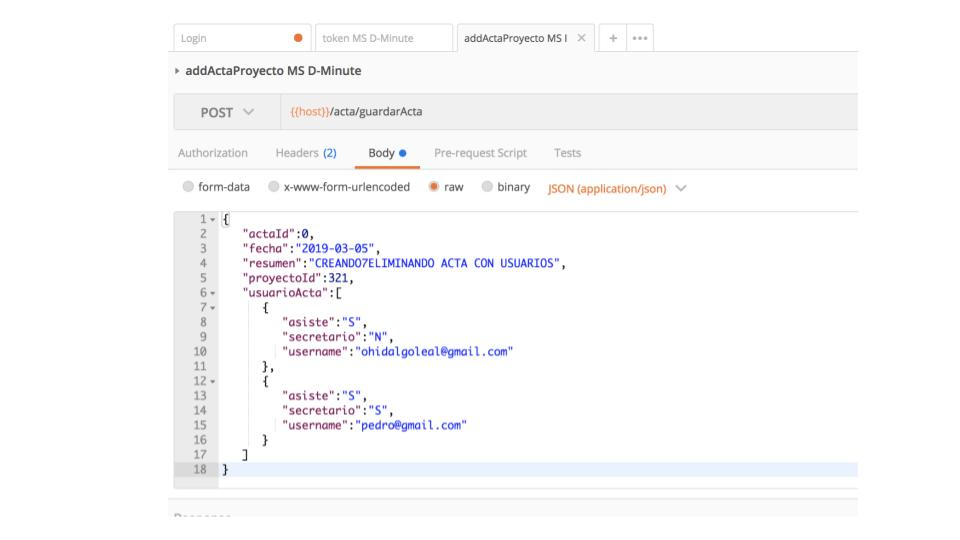
\includegraphics[width=0.8\linewidth]{/postmand}
\label{imga-c2}
\caption{Demostración servicio creación de acta, elaboración propia}
\end{figure}

\end{itemize}


	\item \textbf{\textit{Sprint} 3:} Generar estructura de proyecto \textit{front-end} en angular 5. 

\begin{itemize}
\item \textit{Spring Backlog}

\begin{table}[!h]
\centering
\label{tab:backlog3}
\begin{tabular}{|l|l|r|}
\hline
\multicolumn{1}{|c|}{\textit{\textbf{Feature}}} & \textbf{Epica} & \textbf{Peso} \\ \hline
Implementación nueva estructura UX & Técnica & 8 \\ \hline
Eliminar envio de correo en creación usuario & Técnica & 3 \\ \hline
Cambiar librería de input de textos & Generación Acta & 3 \\ \hline
\textit{Spike} -  Revisar librería Kanban tareas & Seguimiento de tareas & 2 \\ \hline
\end{tabular}
\end{table}

\item Desarrollo: Para el desarrollo de este \textit{sprint} no hubo intenciones de aumentar la velocidad como en el \textit{sprint} anterior debido a que la complejidad de migrar código de un lenguaje a otro es bastante complejo además de que parte del equipo estaría enfocado en investigación (\textit{spike}) con el objetivo de revisar la implementación de un tablero Kanban para el seguimiento de tareas que derivan de los compromisos individuales. La implementación de esta nueva estructura de UX tiene relación a la migración de código python a código angular 5 lo que convella a generar la estructura de carpeta y módulos necesarios para la base de nuestro front-end, uso de nuevas librerías para cuadros de texto y eliminar durante la migración de código el envío de correo en la generación de actas. Lo que corresponde al \textit{spike} se investigó librerías desarrolladas en node, java script y python sin resultados esperados.

\item \textit{Spring Review}: Para el desarrollo de este \textit{sprint} hubo avances significativos de cara al \textit{front-end}. Se presenta su estructura de proyecto en angular 5 y el despliegue del mismo en Heroku. Para el spike si bien se encontró documentación no se pudo seguir investigando pues el equipo se enfocó en terminar el desarrollo de las HDU por tanto no se completaron todos los puntos del \textit{sprint}.

\begin{figure}[!h]
\centering
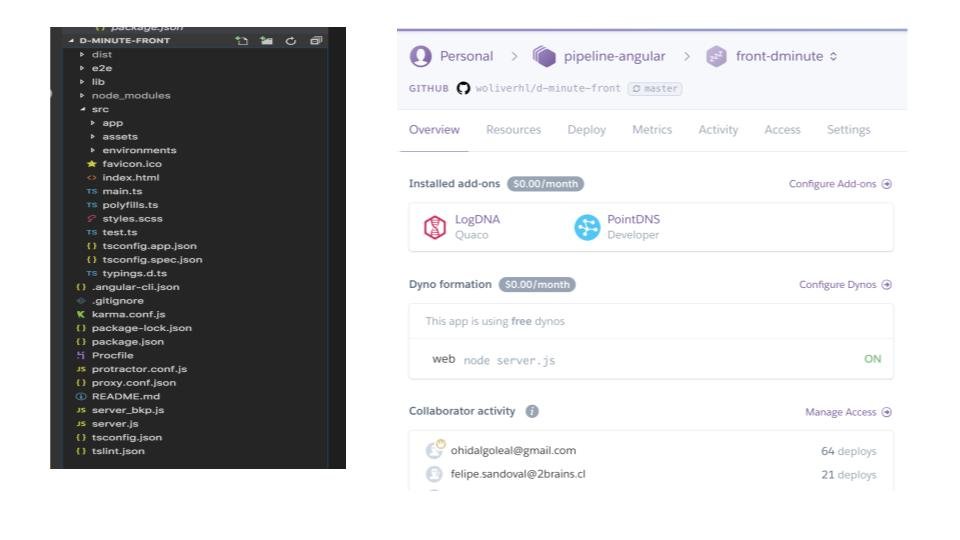
\includegraphics[width=0.8\linewidth]{/demosprint3}
\label{imga-c3}
\caption{Proyecto angular y despliegue en Heroku, elaboración propia}
\end{figure}

\end{itemize}


	\item \textbf{\textit{Sprint} 4:} Migrar por completa aplicación de python a microarquitectura e implementar modelo final de base datos. 

\begin{itemize}
\item \textit{Spring Backlog}

\begin{table}[!h]
\centering
\label{tab:backlog4}
\begin{tabular}{|l|l|r|}
\hline
\multicolumn{1}{|c|}{\textit{\textbf{Feature}}} & \textbf{Epica} & \textbf{Peso} \\ \hline
Reestructurar Menú Creación de Actas & Evolución UX & 5 \\ \hline
Reestructurar Listado de Minutas & Evolución UX & 8 \\ \hline
\end{tabular}
\end{table}

\item Desarrollo: Durante el desarrollo de este \textit{sprint} se abordó la parte front-end de acuerdo a la nueva estructura de UX diseñada previo al \textit{sprint} uno y complementada con el desarrollo de API`s del \textit{sprint} anterior. Dado el nuevo diseño fue necesario generar el modelo final de la base datos que aborda desde el inicio de sesión, el listado de proyectos, las actas de reunión y los elementos del diálogo de cada tema. 

El nuevo diseño de la aplicación llevó a construir la primera parte visual del prototipo, lo anterior generó una tarea bastante complicada que estaba relacionada a la creación de un servidor nginex\footnote{Servidor Nginex: \url{https://es.wikipedia.org/wiki/Nginx}} para que Heroku pudiese desplegar la aplicación en Angular 5 de forma correcta.

\item \textit{Spring Review}: Este es sin duda un \textit{sprint} importante pues se logró visualizar el primer prototipo de la aplicación en base al diseño de UX generado. Se pudo apreciar el modelo de base datos para la creación de actas dialógicas y se logró finalizar los puntos comprometidos de manera exitosa durante el \textit{sprint} (ver figuras: C4, C5 y C6).

\begin{figure}[!h]
\centering
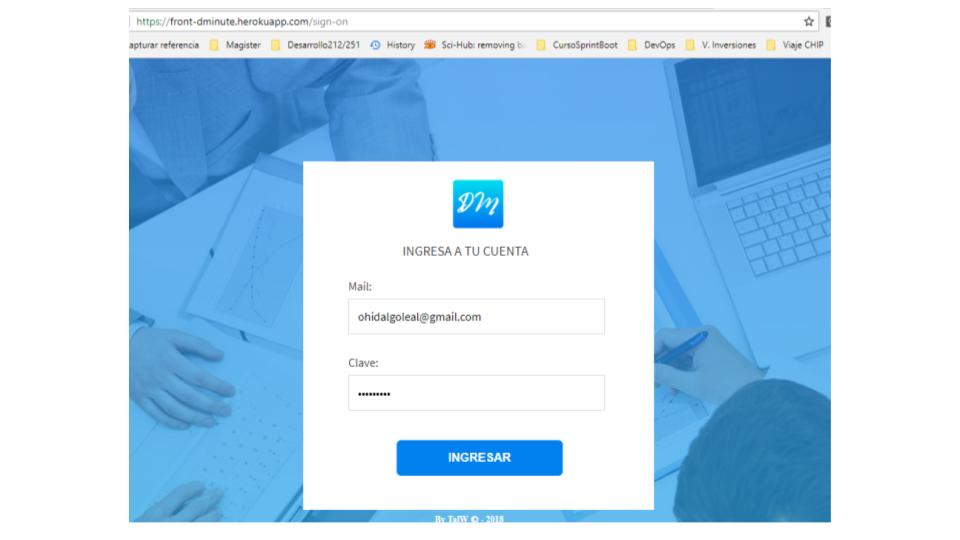
\includegraphics[width=0.8\linewidth]{/demo4-1}
\label{imga-c41}
\caption{Login D-Minute, elaboración propia}
\end{figure}

\begin{figure}[!h]
\centering
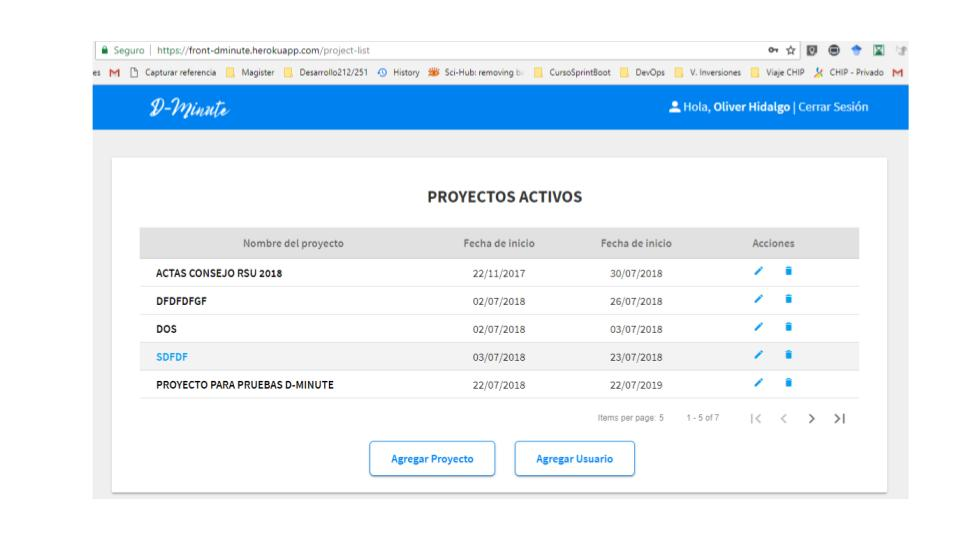
\includegraphics[width=0.8\linewidth]{/demo4-2}
\label{imga-c42}
\caption{Listado proyectos D-Minute, elaboración propia}
\end{figure}

\begin{figure}[!h]
\centering
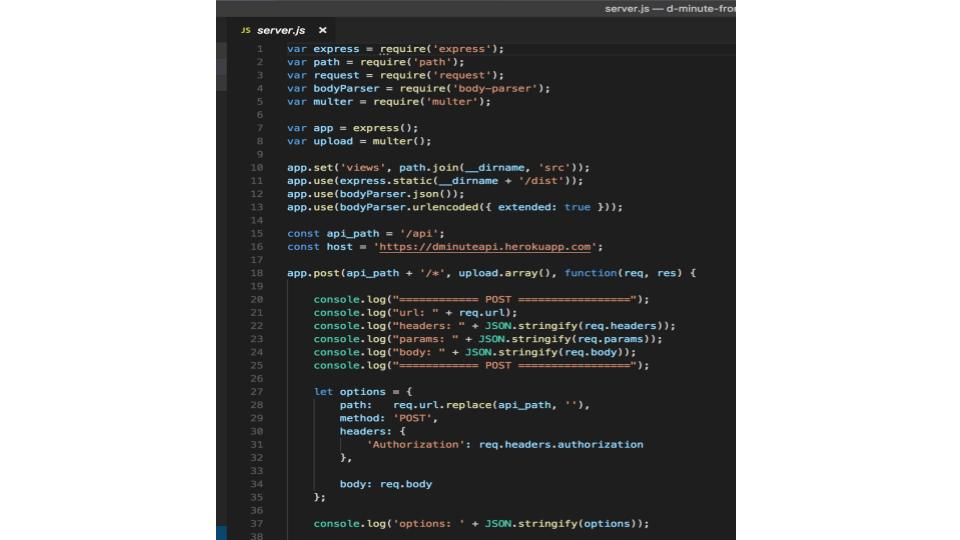
\includegraphics[width=0.8\linewidth]{/demo4-3}
\label{imga-c43}
\caption{Configuración servidor Nginex D-Minute, elaboración propia}
\end{figure}

\end{itemize}


	\item \textbf{\textit{Sprint} 5:} Implementar modelo de micro servicios en \textit{cloud} y generar estilos estándar de la aplicación.

\begin{itemize}
\item \textit{Spring Backlog}

\begin{table}[!h]
\centering
\label{tab:backlog5}
\begin{tabular}{|l|l|r|}
\hline
\multicolumn{1}{|c|}{\textit{\textbf{Feature}}} & \textbf{Epica} & \textbf{Peso} \\ \hline
Normalizar colores aplicación & Evolución UX & 5 \\ \hline
Cargar usuarios nuevos al crear un proyecto & Generación Acta & 5 \\ \hline
Visualizar detalle minuta & Evolución UX & 8 \\ \hline
\end{tabular}
\end{table}

\item Desarrollo: En los \textit{sprint} anteriores hubo un fuerte trabajo por realizar la migración del código desarrollado en python a una nueva arquitectura en java con angular utilizando microsiervos. Este \textit{sprint} está marcado por este último factor, pues era importante comenzar a montar el diseño de arquitectura que hace sostenible la aplicación. Fue necesario comenzar a trabajar en la creación del config server, el registro de eureka y zuul como \textit{proxy server}, todos ellos dentro de un servidor \textit{cloud} Heroku que hace eficiente el desempeño de la aplicación y escalable. 

A los puntos anteriores se suma la creación de minutas, los elementos de diálogo mencionados en el CAPÍTULO 2 sección 2.2 y por último se comenzó a estandarizar los colores de la aplicación reduciendo la deuda técnica adquirida en \textit{sprint} anteriores.

\item \textit{Spring Review}: Durante la \textit{review} de este \textit{sprint} se presentó los componentes desplegados en Heroku que soportan los microservicios que fueron configurados dentro de un pipeline\footnote{Definición y uso de pipeline en: \url{https://jenkins.io/doc/book/pipeline/}} de java y la visualización gráfica de las minutas de un proyecto (ver figuras: C7 y C8).

\begin{figure}[!h]
\centering
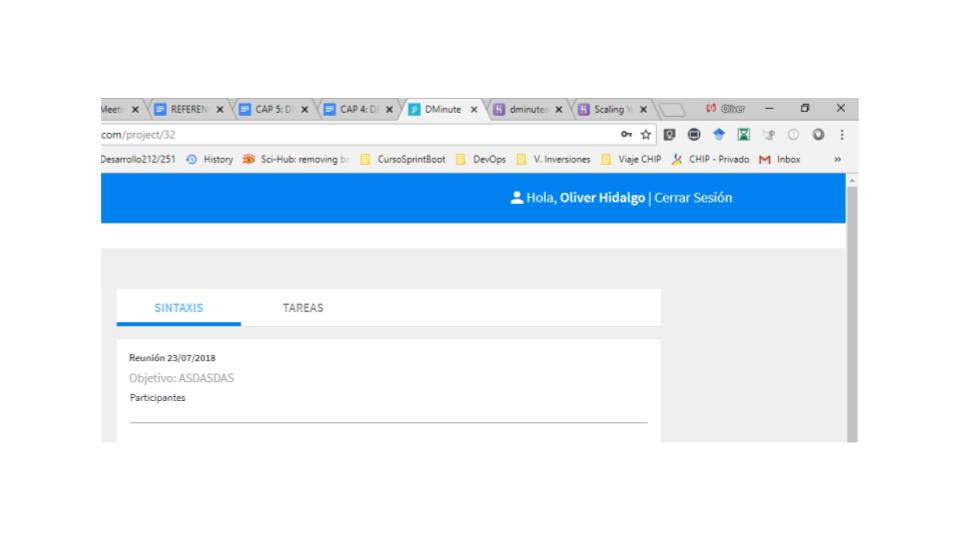
\includegraphics[width=0.8\linewidth]{/demo5-1}
\label{imga-c51}
\caption{Visualizar detalle acta D-Minute, elaboración propia}
\end{figure}

\begin{figure}[!h]
\centering
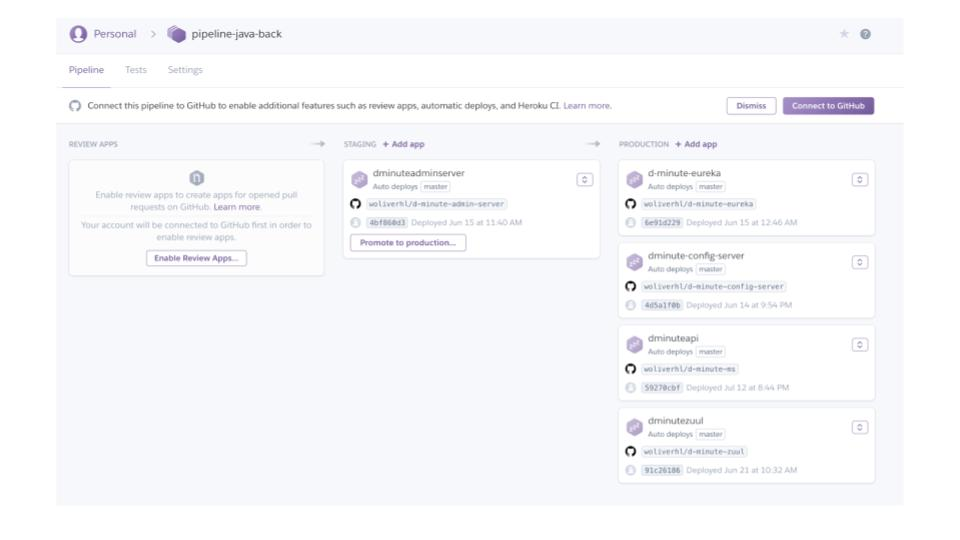
\includegraphics[width=0.8\linewidth]{/demo5-2}
\label{imga-c52}
\caption{Pipeline arquitectura de microservicios D-Minute, elaboración propia}
\end{figure}

\end{itemize}


	\item \textbf{\textit{Sprint} 6:} Mejorar aspectos visuales de la aplicación arrastrados de la migración. 
	
\begin{itemize}
\item \textit{Spring Backlog}

\begin{table}[!h]
\centering
\label{tab:backlog6}
\begin{tabular}{|l|l|r|}
\hline
\multicolumn{1}{|c|}{\textit{\textbf{Feature}}} & \textbf{Epica} & \textbf{Peso} \\ \hline
Texto al agregar elementos de diálogo & Generación Acta & 1 \\ \hline
Eliminación Menú & Evolución UX & 1 \\ \hline
BUG: editar un elemento de diálogo & Generación Acta & 3 \\ \hline
Quitar opción colapsable & Evolución UX & 5 \\ \hline
Nombre en barra superior & Evolución UX & 2 \\ \hline
Calendario en español & Generación Acta & 3 \\ \hline
\end{tabular}
\end{table}

\item Desarrollo: El desarrollo del \textit{sprint} 6 está marcado por mejorar aspectos visuales de la aplicación pues producto de la migración a java y angular algunas características de la aplicación se tomaron de python sin ser cuestionadas. Si bien el producto pretende ser un mínimo viable, se testeó la aplicación con algunos usuarios finales durante el \textit{sprint} 5 lo que permitió incorporar en esta\textit{sprint backlog} historias que permitan mejorar la experiencia de usuario también durante el testeo se detectaron \textit{BUG} que fueron abordados en el \textit{sprint}.

\item \textit{Spring Review}: Como se indicó en el desarrollo, las mejoras del producto fue el punto a revisar durante el \textit{sprint} y los BUG identificados por los usuarios finales (ver figura C9).

\begin{figure}[!h]
\centering
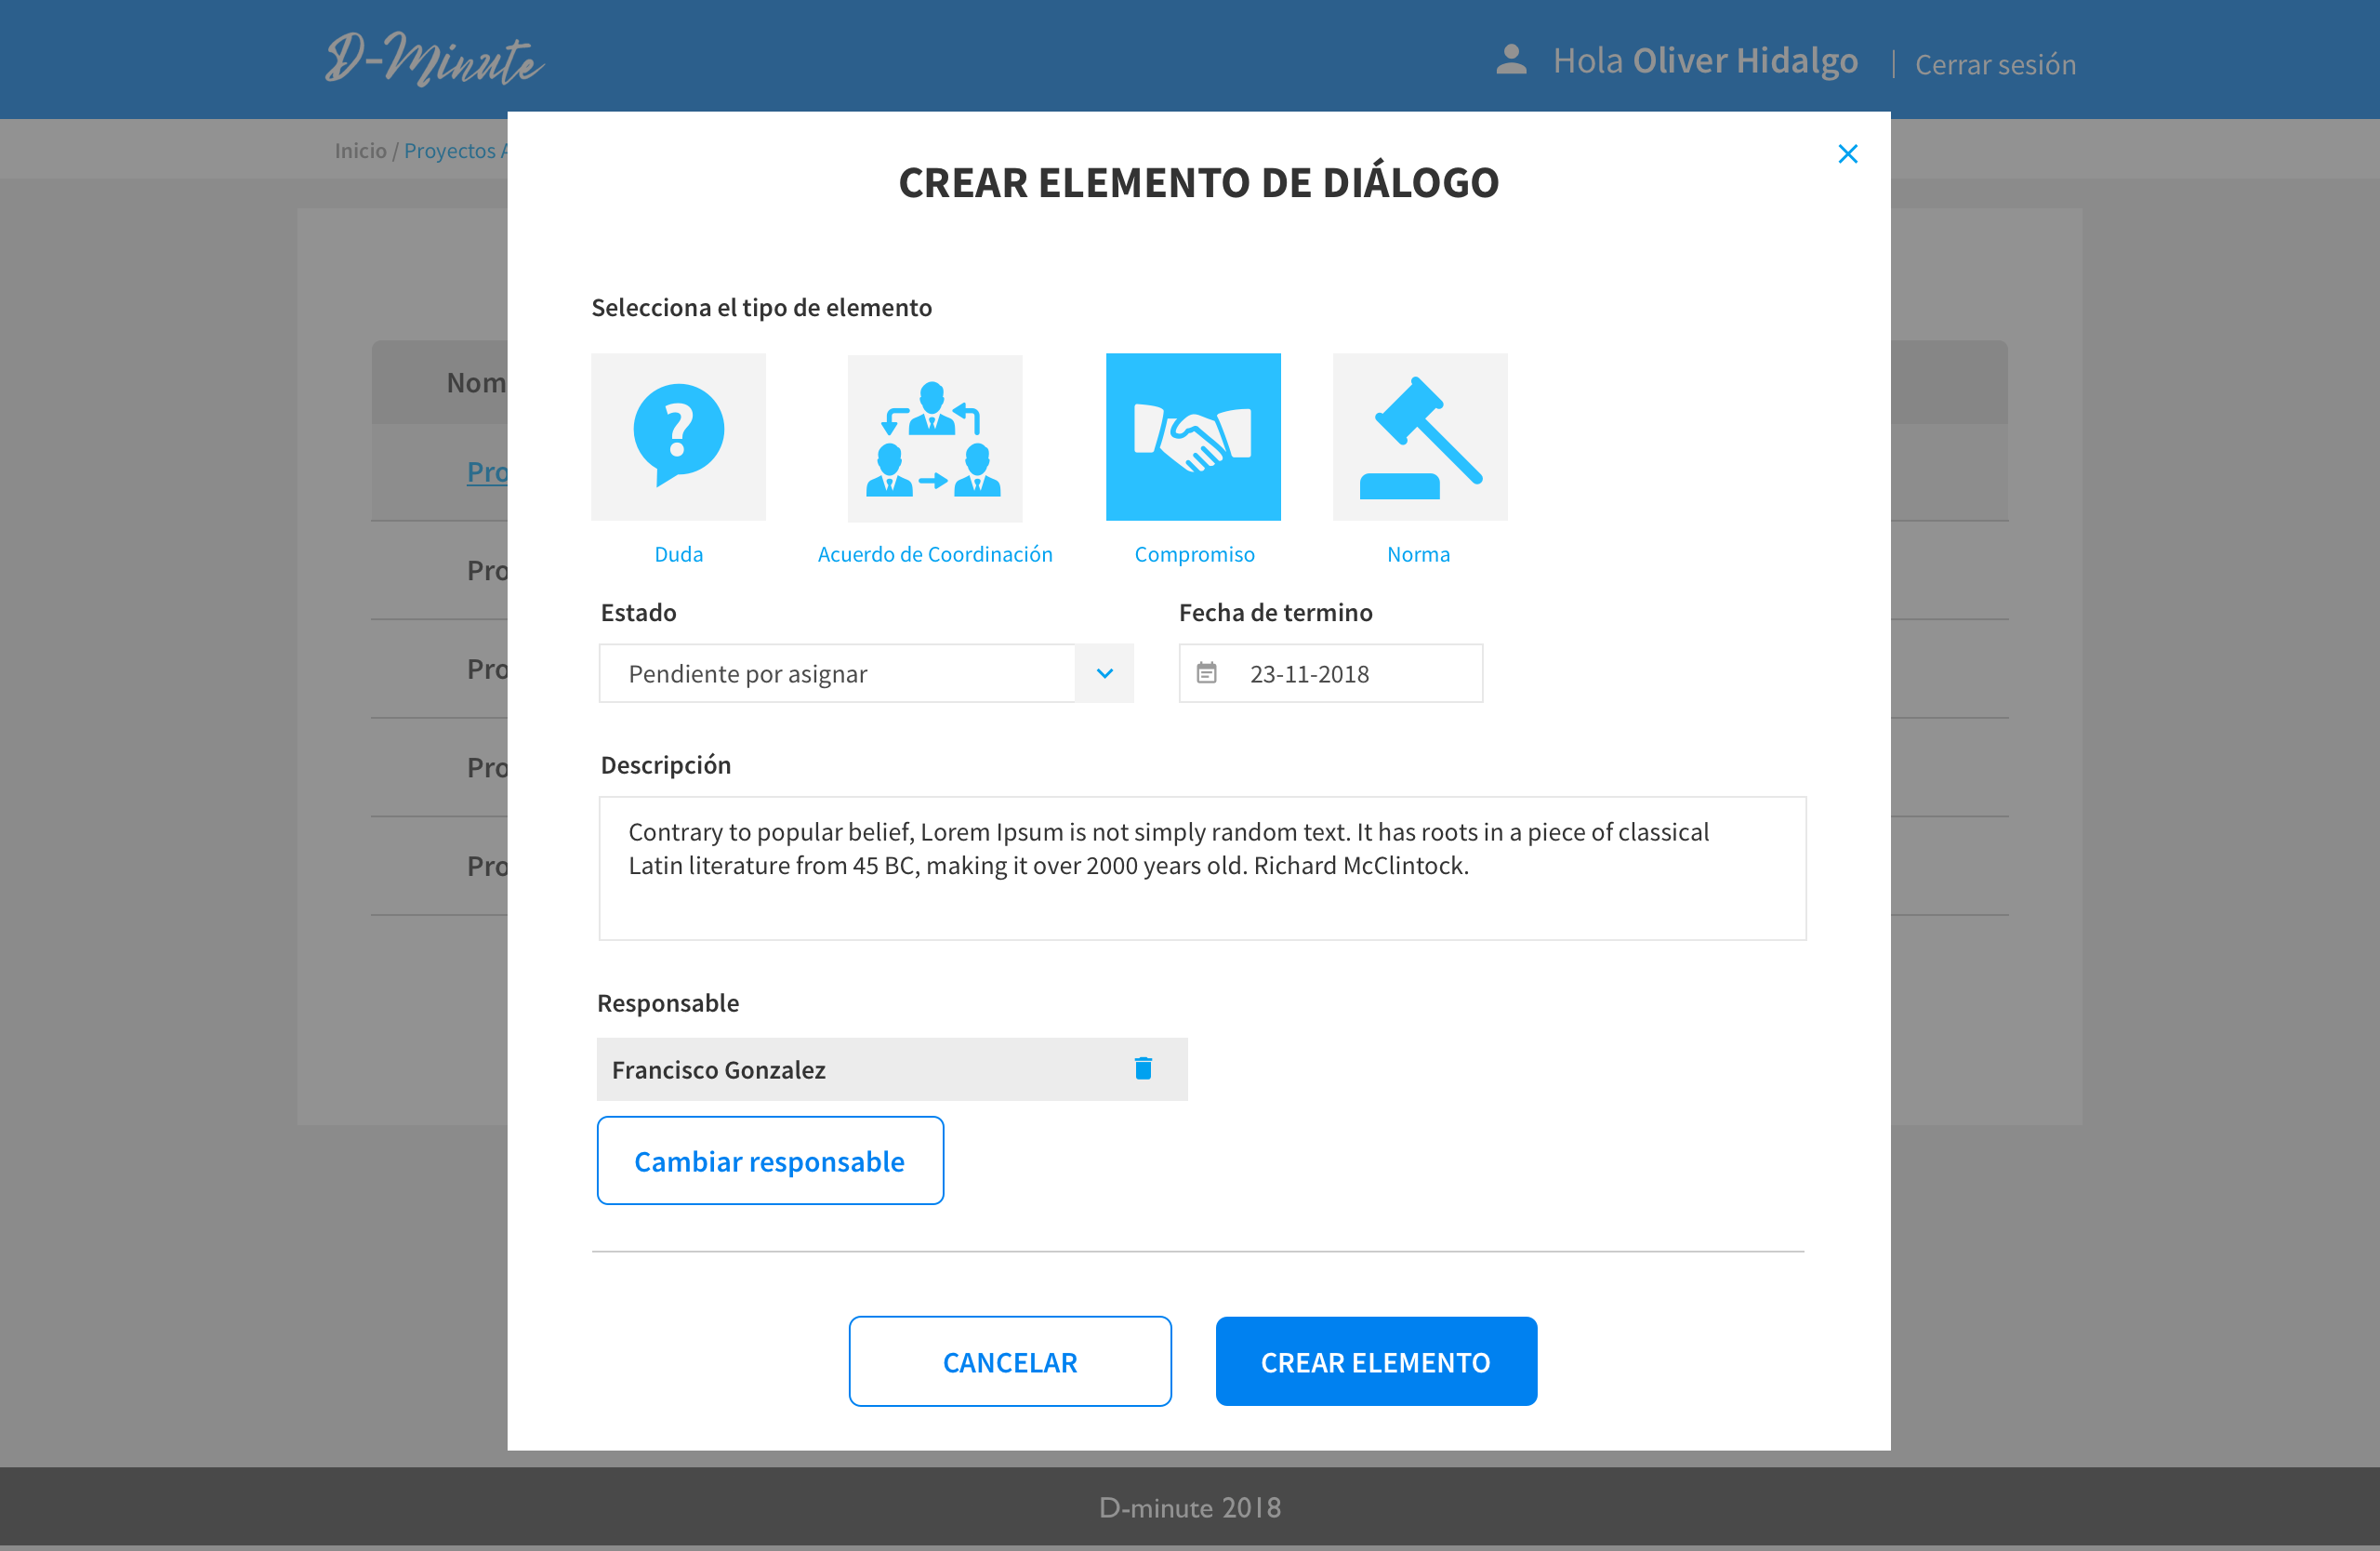
\includegraphics[width=0.8\linewidth]{/demo6}
\label{imga-c6}
\caption{Mejoras al editar elementos de diálogo D-Minute, elaboración propia}
\end{figure}

\end{itemize}	

	\item \textbf{\textit{Sprint} 7:} Implementar nuevo diseño UX y corrección de \textit{bugs} críticos. 

\begin{itemize}
\item \textit{Spring Backlog}

\begin{table}[!h]
\centering
\label{tab:backlog7}
\begin{tabular}{|l|l|r|}
\hline
\multicolumn{1}{|c|}{\textit{\textbf{Feature}}} & \textbf{Epica} & \textbf{Peso} \\ \hline
BUG: seleccionar asistentes de una reunión & Generación Acta & 5 \\ \hline
BUG: al editar y crear un acta & Generación Acta & 5 \\ \hline
Mejora estilo + iconos & Evolución UX & 8 \\ \hline
BUG: Se duplica acta al editar & Generación Acta & 5 \\ \hline
\end{tabular}
\end{table}


\item Desarrollo: Durante el \textit{sprint} 5 y 6 se comenzó el testeo de la aplicación con usuarios finales a fin de identificar puntos de mejora que no se detectaron durante el QA de la aplicación. Resultado de este trabajo fueron \textit{BUGs} importantes que afectaron la funcionalidad del producto y debido a que eran críticos se priorizo la corrección de estos por sobre nuevas funcionalidades, sin embargo debido al mismo testeo de usuarios se incorporó la nueva línea UX en la aplicación pues era la apuesta principal que se apuntaba como equipo, un hito importante considerando que hubo un sobre esfuerzo en términos de\textit{velocity}. 

\item \textit{Spring Review}: El resultado de este \textit{sprint} es sin lugar a dudas uno de los más importantes pues se logró implementar la nueva línea de UX que fue testeada con los usuarios finales. Se marca un cambio en la forma de visualizar las minutas y se incorporan los nuevos iconos de los elementos de diálogo sin dejar de lado los bugs detectados en etapas tempranas (ver figura C10).

\begin{figure}[!h]
\centering
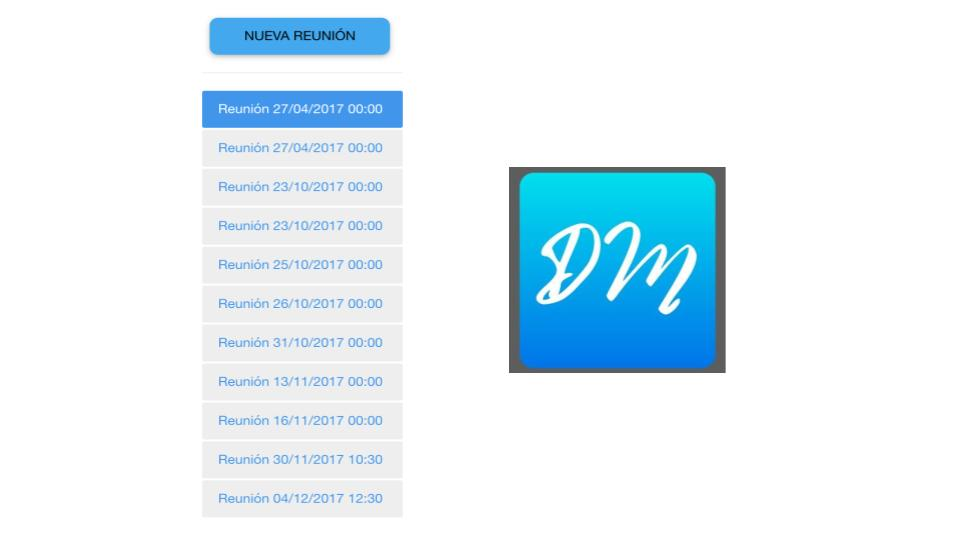
\includegraphics[width=0.8\linewidth]{/demo7}
\label{imga-c7}
\caption{Nuevo logo D-Minute y lista de reuniones, elaboración propia}
\end{figure}

\end{itemize}	


	\item \textbf{\textit{Sprint} 8:} Reducir deuda técnica de \textit{front-end} y \textit{back-end}. 

\begin{itemize}
\item \textit{Spring Backlog}

\begin{table}[!h]
\centering
\label{tab:backlog8}
\begin{tabular}{|l|l|r|}
\hline
\multicolumn{1}{|c|}{\textit{\textbf{Feature}}} & \textbf{Epica} & \textbf{Peso} \\ \hline
Seleccionar Icono al agregar elemento de diálogo & Trazabilidad Elementos & 8 \\ \hline
BUG: Se corta pantalla al agregar elemento de diálogo & Evolución UX & 3 \\ \hline
Quitar espaciado Panel de Proyecto & Evolución UX & 2 \\ \hline
Número reunión & Generación Acta & 5 \\ \hline
\end{tabular}
\end{table}



\item Desarrollo: Nuestro último \textit{sprint} está marcado por mejoras en la aplicación y deuda técnica de backend que eran necesarias para mejorar performance del software, de igual forma se trabajó en aspecto de experiencia de usuario pues una de las características de la aplicación es el concepto usable para ello las HDU indicadas abordan este concepto. Los bug detectados fueron desarrollados por el equipo pero no tenían una alta complejidad como los indicados en el \textit{sprint} anterior.

Lo anterior, permitió al equipo volver a su velocidad de 16 puntos por sobre el esfuerzo extra realizado el \textit{sprint} anterior que el objetivo era concluir la nueva línea de UX.

\item \textit{Spring Review}: La \textit{review} de este \textit{sprint} se enmarca dentro de las mejoras de la aplicación por tanto se presenta al PO los bugs detectados haciendo hincapié en los aspectos técnicos que mejoran la performance de la aplicación.

\end{itemize}

\end{itemize}


\section{\textit{Questionnaire for User Interface Satisfaction}}

El \textit{software} D-Minute, a pesar de no haber generado el experimento para validar hipótesis científica, está siendo utilizado en dos empresas del mercado, por personas que a diario se ven a enfrentados los problemas descritos en capítulos anteriores. A ellos, se les aplicó una encuesta de satisfacción (abreviada en ingles: QUIS) para entregar más antecedentes a la hora de evaluar científicamente la aplicación o generar mejoras al producto.

\subsection{QUIS Colaboradores Caja de Compensación}



\subsection{QUIS Colaboradores Banco}

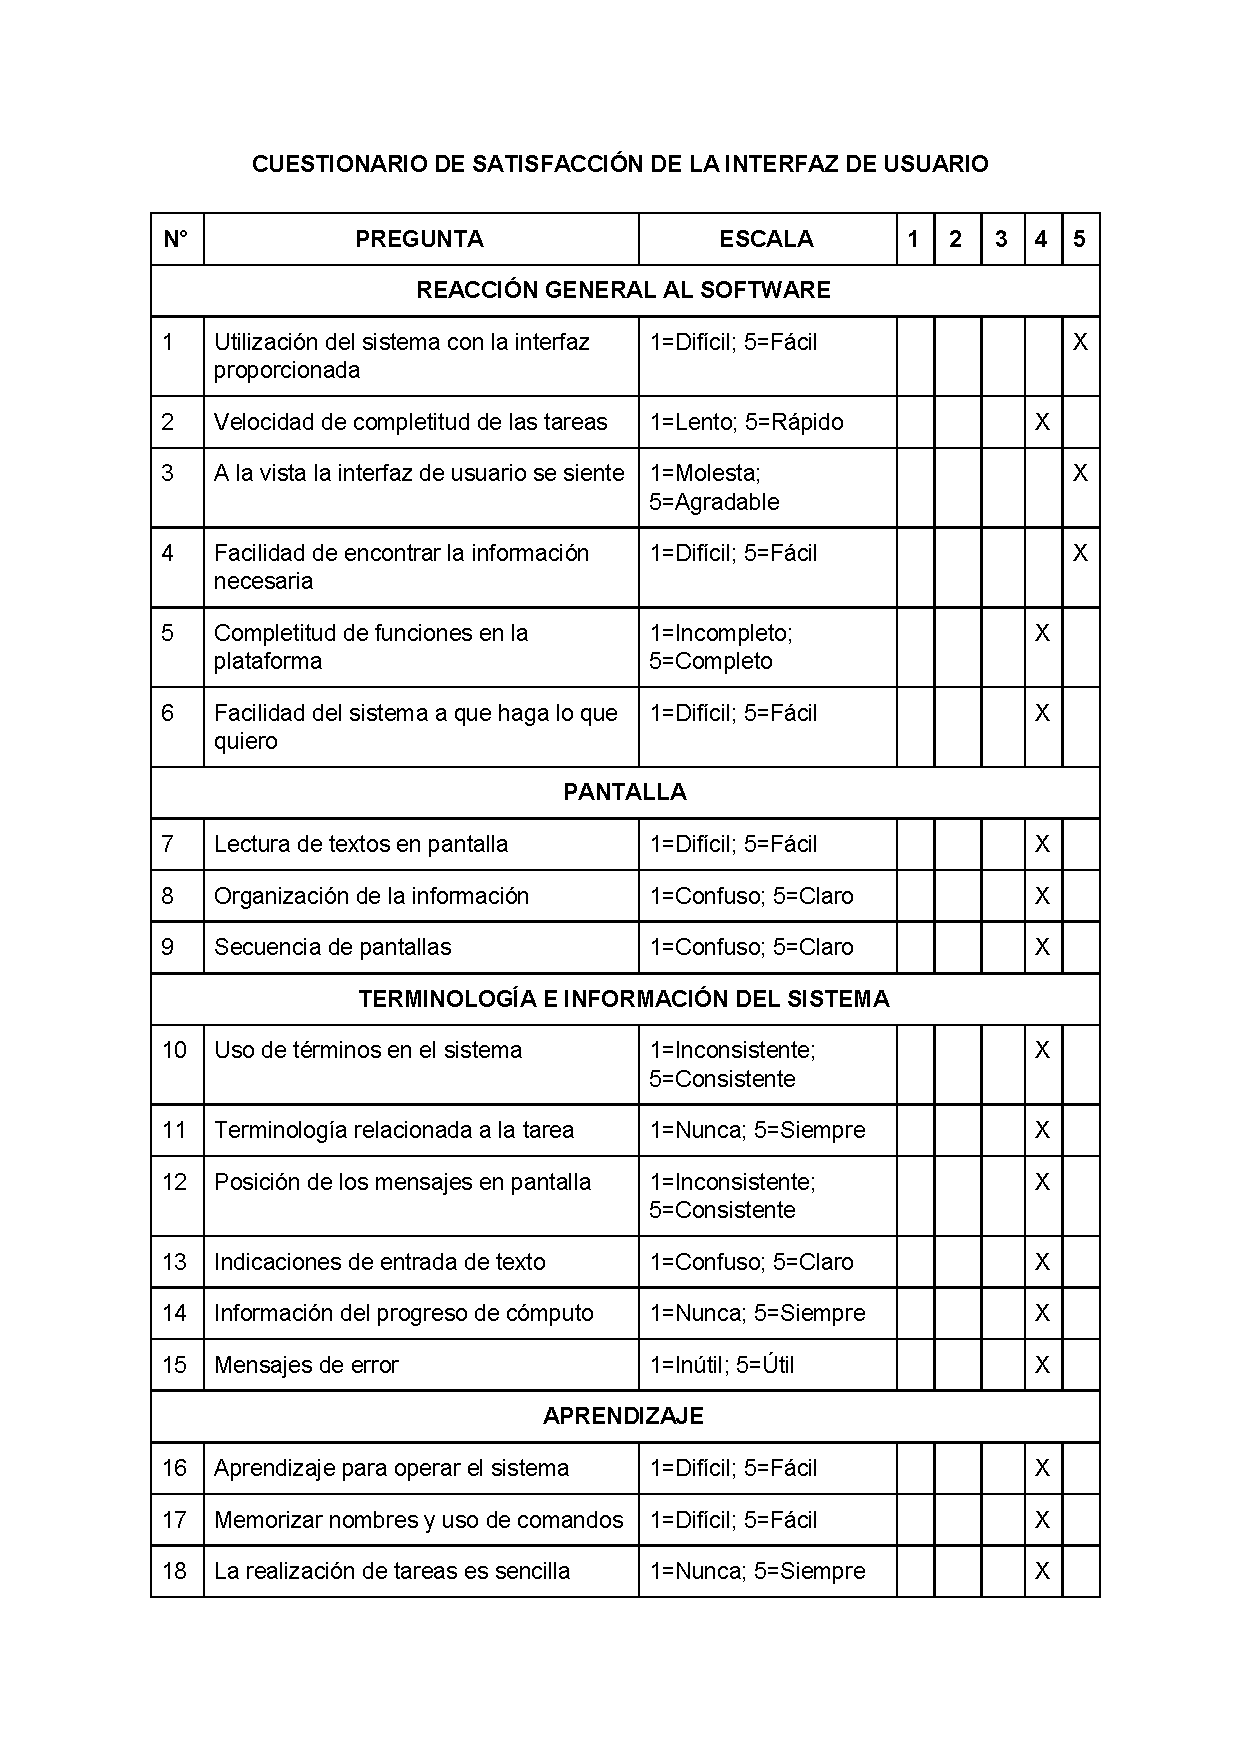
\includepdf{Figures/pdf/QUIS_MarcelaGonzalez_BCI}
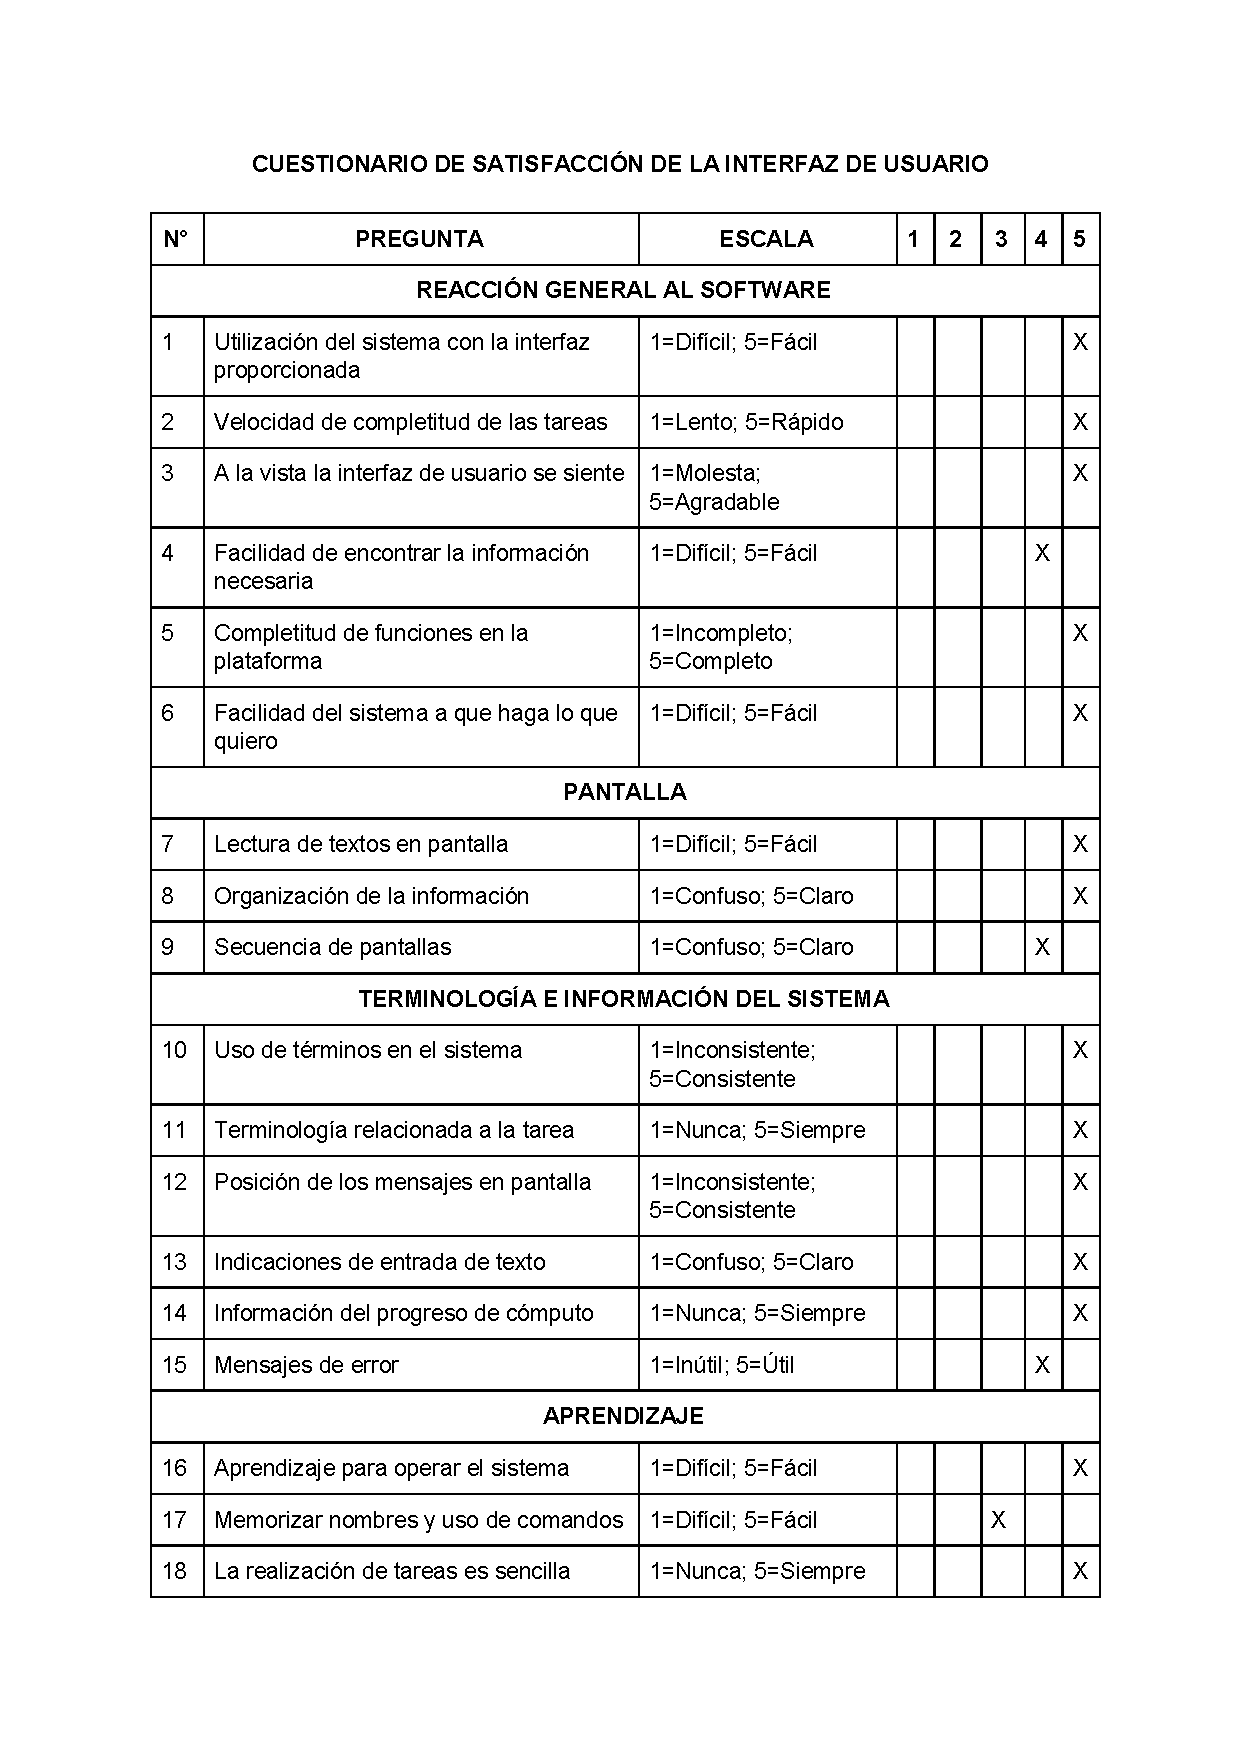
\includepdf{Figures/pdf/QUIS_OscarMillanao_BCI}

%----------------------------------------------------------------------------------------

\end{document}